% !TeX spellcheck = de_DE
\documentclass[a4paper,12pt,numbers=noenddot,parskip=full]{scrartcl}
 
\usepackage[utf8]{inputenc}
\usepackage[T1]{fontenc}
\usepackage{lmodern}
\usepackage[ngerman]{babel}
\usepackage{color}
\usepackage[hidelinks]{hyperref}
\usepackage{amsmath,amssymb,amstext,mathtools,amsthm}
\usepackage{subcaption}
\usepackage{float}
\usepackage{wasysym}
\usepackage{stmaryrd}
\usepackage{bbm}
\hypersetup{bookmarksnumbered}



\usepackage{tikz}
\usetikzlibrary{positioning}
\usetikzlibrary{arrows}

\usepackage{enumitem}
\setenumerate{label=\arabic*)}

\newcommand{\setN}{\mathbb{N}}
\newcommand{\setZ}{\mathbb{Z}}
\newcommand{\setQ}{\mathbb{Q}}
\newcommand{\setR}{\mathbb{R}}
\newcommand{\setC}{\mathbb{C}}
\newcommand{\setH}{\mathbb{H}}
\newcommand{\setk}{\Bbbk}
\newcommand{\ldot}{\,.\,}
\newcommand{\Forall}{~\forall}
\newcommand{\Exists}{~\exists}

\newcommand{\abs}[1]{{\left| #1 \right|}}
\newcommand{\dabs}[1]{{\left\lVert #1 \right\rVert}}
\newcommand{\heading}{\underline}
 
\DeclareMathOperator{\Kons}{Kons}
\DeclareMathOperator{\charac}{char}
\DeclareMathOperator{\Gal}{Gal}

\newtheoremstyle{dotless}{}{}{\itshape}{}{\bfseries}{}{ }{}
 
\theoremstyle{dotless}
\newtheorem{theorem}{Satz}[section]
\newtheorem{corollary}[theorem]{Folgerung}
\newtheorem{proposition}[theorem]{Proposition}
\newtheorem{lemma}[theorem]{Lemma}
\newtheorem{definition}[theorem]{Definition}
\newtheorem{example}[theorem]{Beispiel}
\newtheorem*{axiom}{Axiom}

\makeatletter
\g@addto@macro\th@remark{\thm@headpunct{:}}
\makeatother 
\theoremstyle{remark}
\newtheorem*{remark}{Bemerkung}
 
\hfuzz=5pt 
 
\title{Algebra und Zahlentheorie}

\subtitle{Wintersemester 2018/19}
\author{gehalten von Prof. Dr. Stefan Kebekus}
\date{\today}
 
\begin{document}
	\pagestyle{headings}
\begin{titlepage}
	\maketitle	
	\thispagestyle{empty}
\end{titlepage}
\tableofcontents 
\thispagestyle{empty}
\newpage
\setcounter{page}{1}
	
	\setcounter{section}{-1}
	\section{Konstruktion mit Zirkel und Lineal}
	
	\begin{example}[Konstruktion des regelmäßigen 5-Ecks]
		Anleitung zur Konstruktion
		\begin{center}
			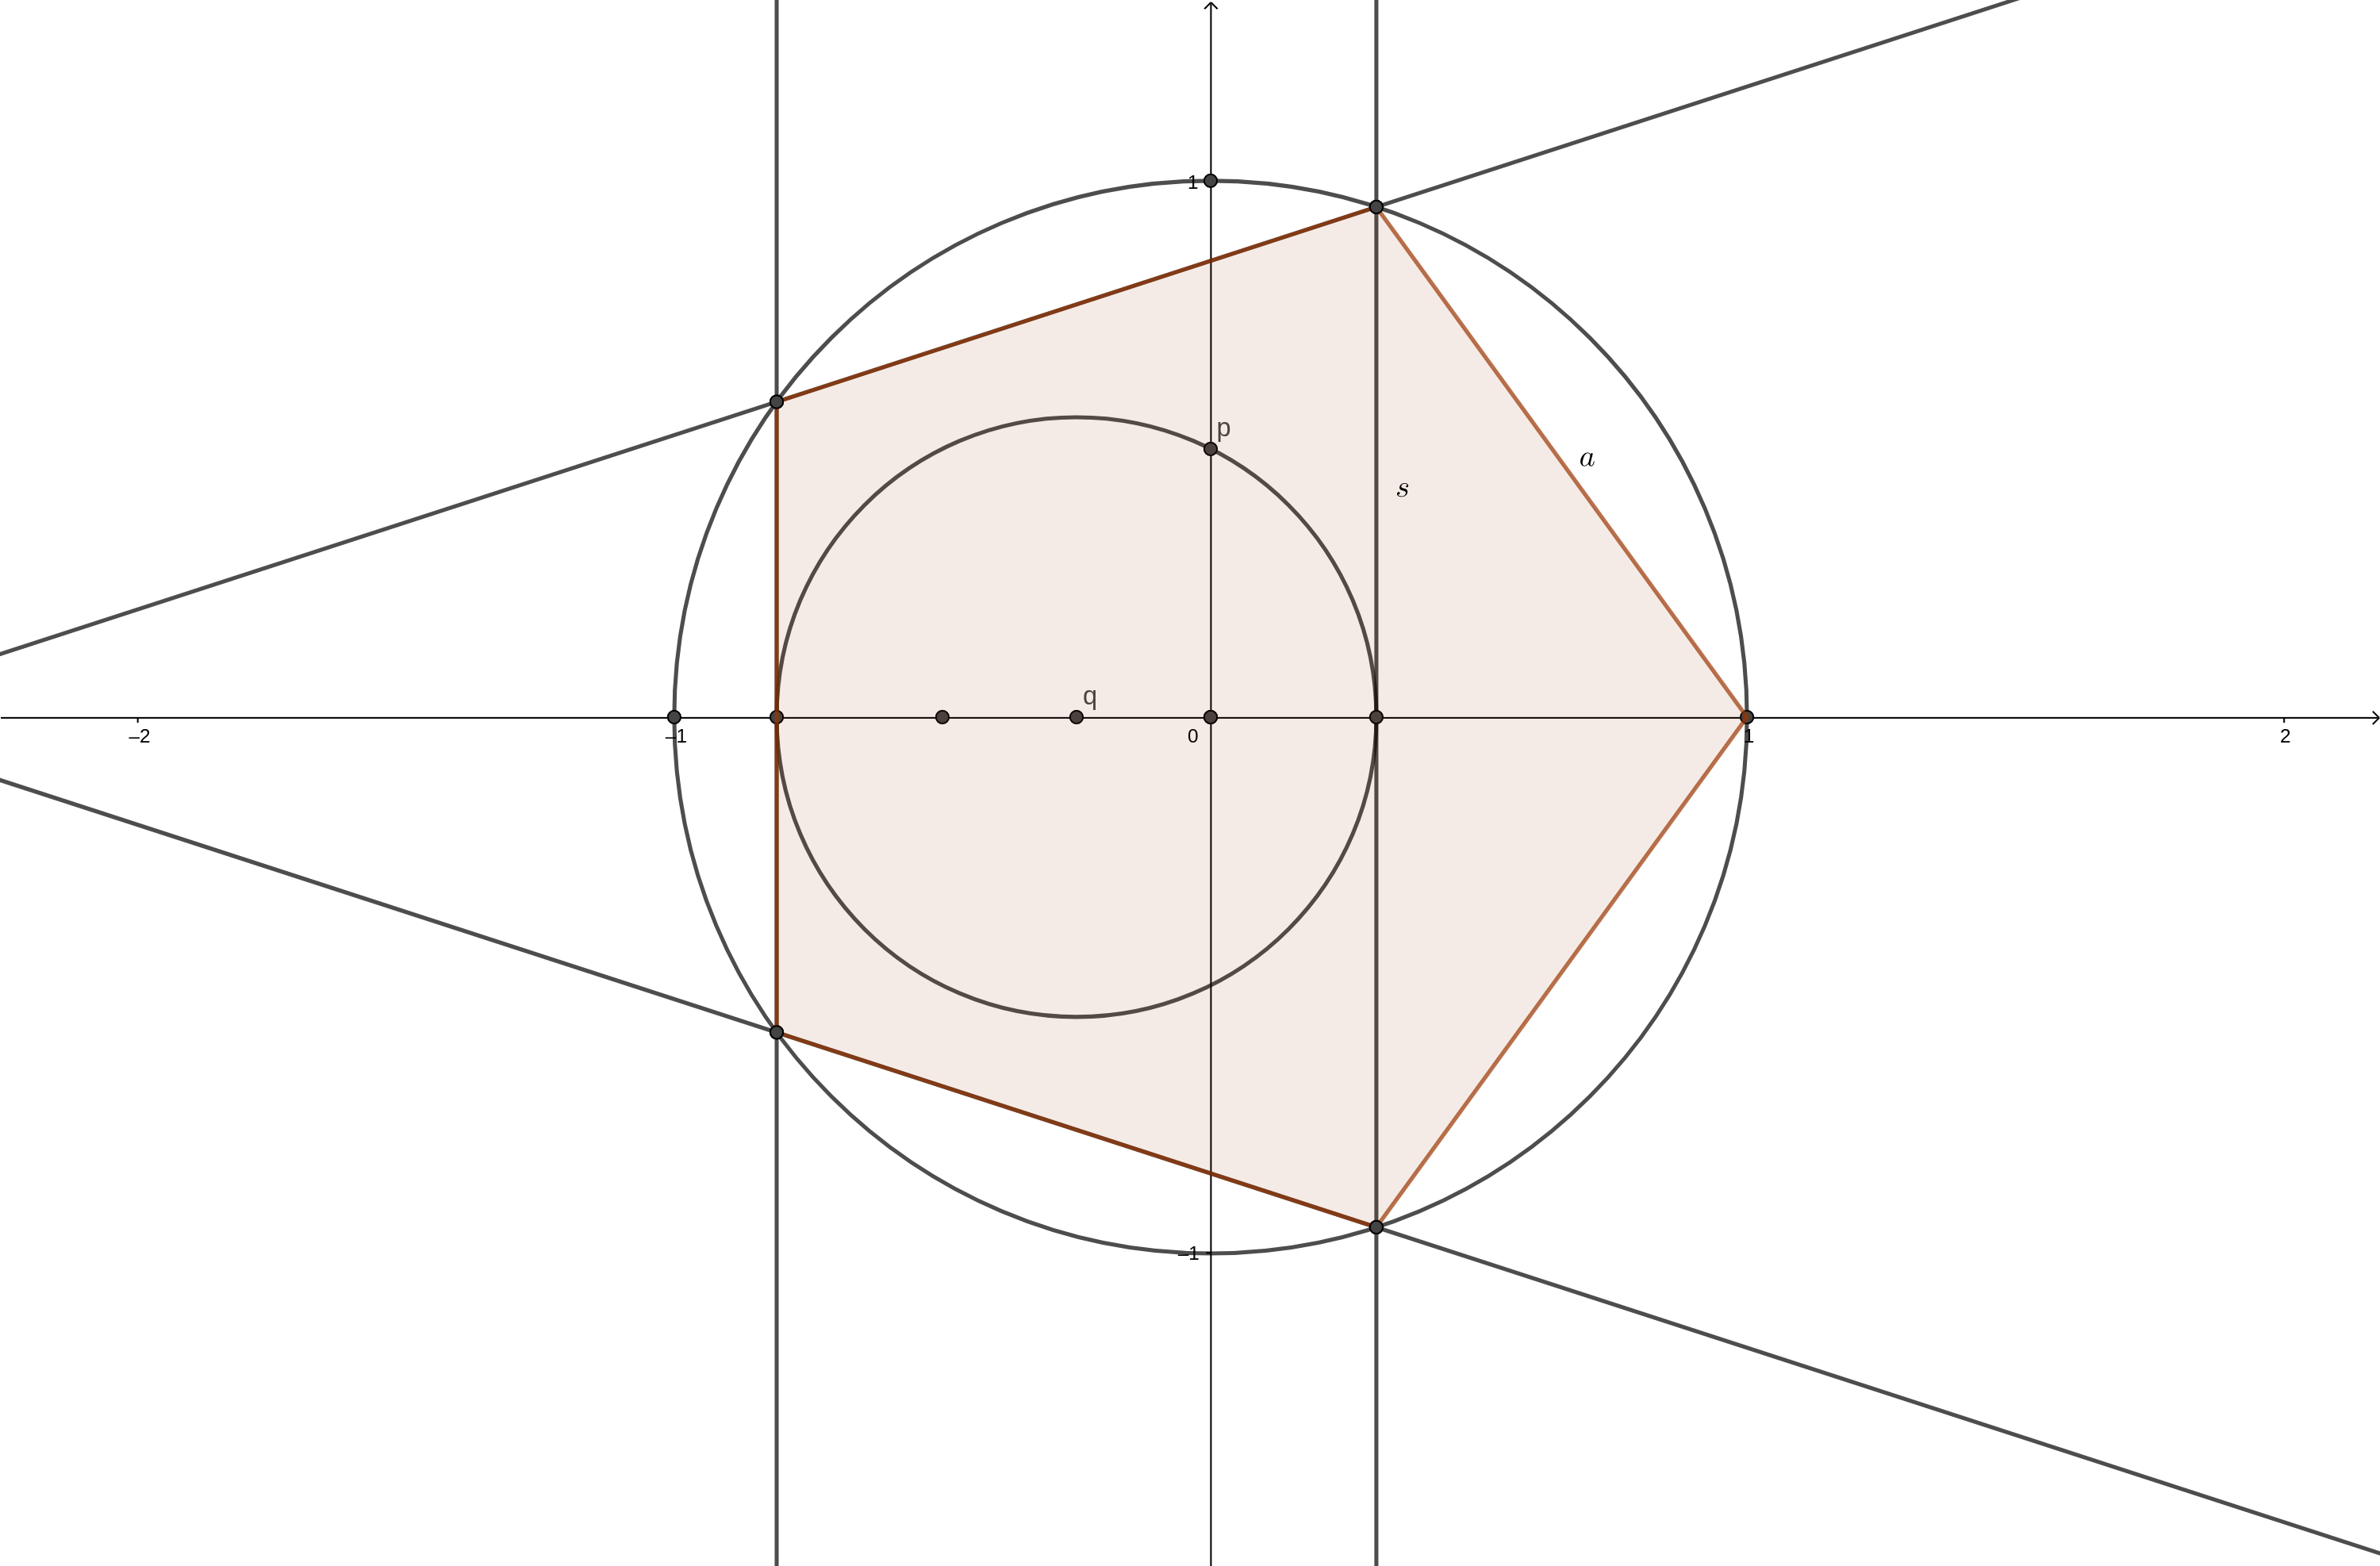
\includegraphics[width=0.8\linewidth]{bilder/bild1.png}
		\end{center}
	\end{example}

	\heading{Erste Frage:} Gegeben $n \in \setN$, kann ich das regelmäßige $n$-Eck konstruieren?
	
	\heading{Beispielproblem:} Betrachte Das $5$-Eck, sei $a$ die Kantenlänge und $s$ die Sekantenlänge.
	
	Dann ist $\frac{s}{a} \notin \setQ$.
	
	\begin{proof}
		Angenommen $\frac{s}{a}$ wäre in $\setQ$. Dann schreibe $\frac{s}{a} = \frac{p}{q}$ mit $p,q \in \setN$. Dann gibt es also eine Länge $d \in \setR$, sodass $s$ und $a$ beide ganzzahlige Vielfache von $d$ sind. $\exists n,m \in \setN$  $a = n \cdot d, s= m \cdot d$.
		
		Betrachte/Erweitere die Konstruktion des $5$-Ecks und erhalte ein kleines $5$-Eck (vgl. blaues $5$-Eck in der Abbildung unten) mit Sekantenlänge $s' = a$ und Kantenlänge $a' = s - a$.
		
		\begin{center}
			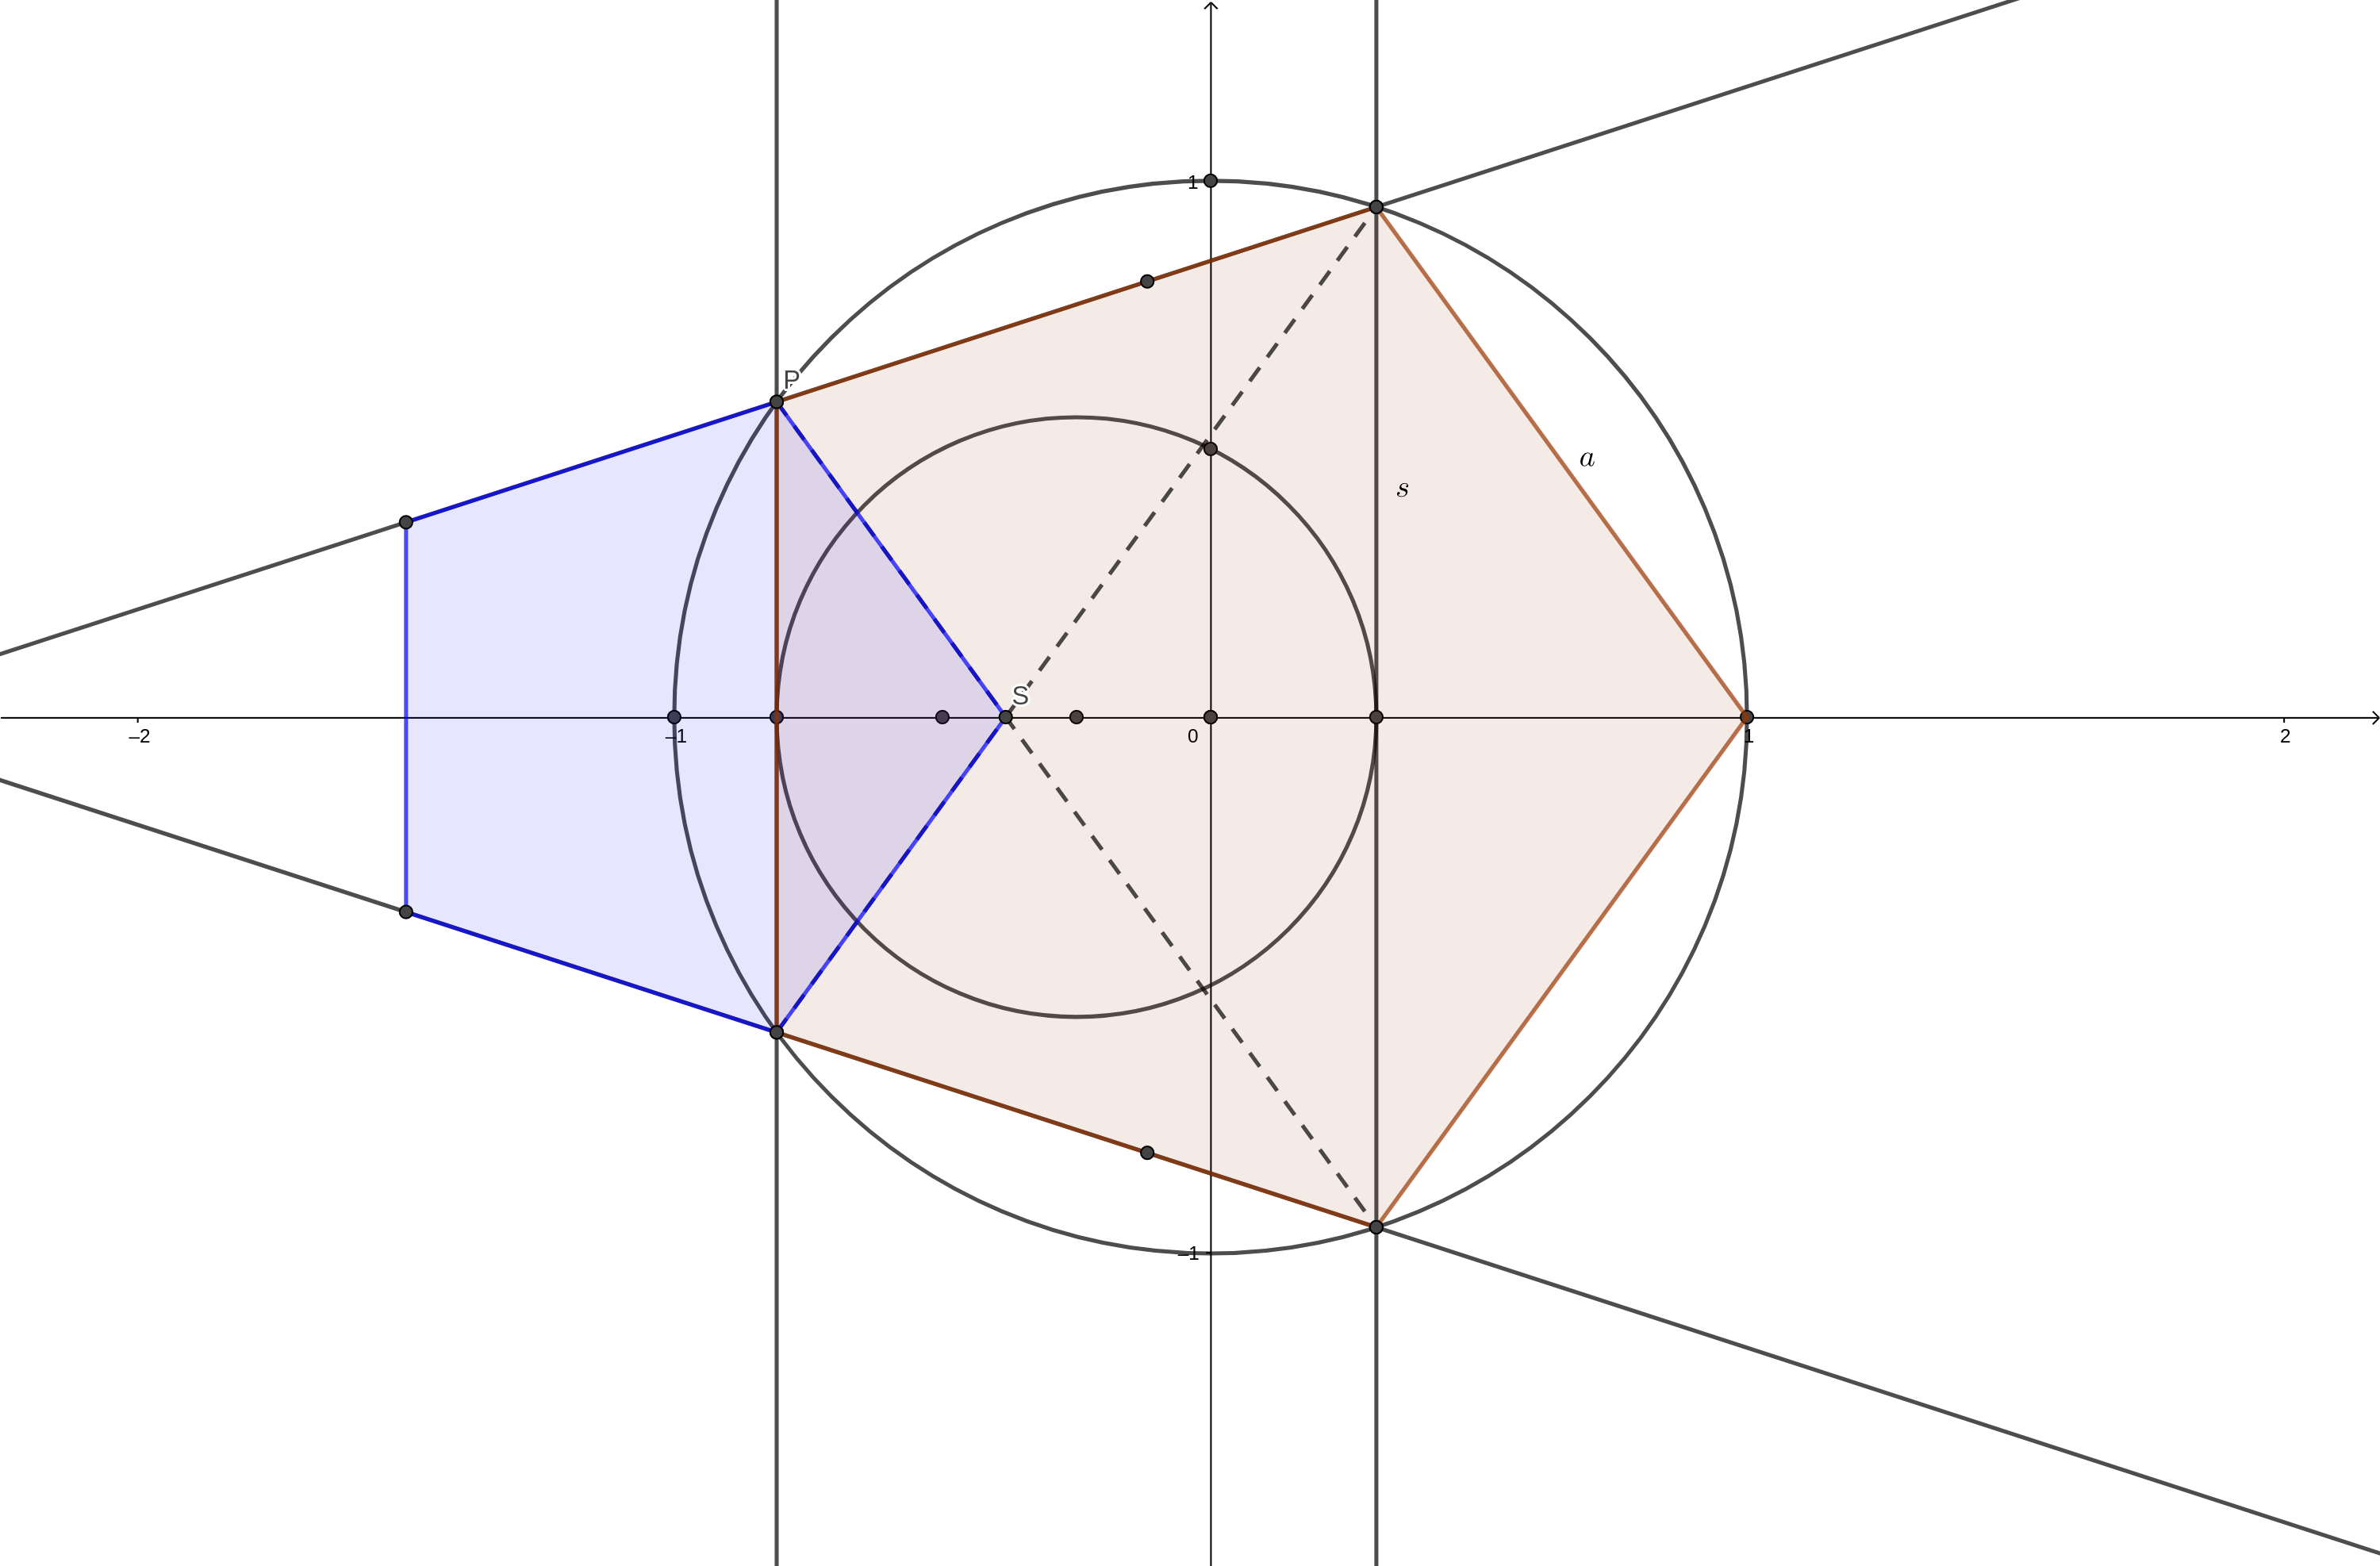
\includegraphics[width=0.8\linewidth]{bilder/bild2.png}
		\end{center}
	
		Dann sind aber sowohl $a'$ als auch $s'$ wieder Vielfache von $d$. Das Verfahren kann ich wiederholen und erhalte immer kleinere $5$-Ecke, deren Größe nach $0$ konvergiert, wo Kanten- und Sekantenlänge ganzzahlige Vielfache von $d$ sind. $\lightning$
	\end{proof}

	\heading{Weitere Konstruktionsprobleme:}
	\begin{itemize}
		\item $3$-Teilung des Winkels
		\item Verdopplung des Würfels (d.h. Verdopplung des Volumens)
		\item Quadratur des Kreises (Gegeben ein Kreis, konstruiere Quadrat mit demselben Flächeninhalt)
	\end{itemize}

	\heading{Wiederholung:} Was kann ich mit Zirkel und Lineal eigentlich machen?
	
	Antwort: $3$ Konstruktionen
	\begin{enumerate}
		\item Gegeben Punkte $a_1, a_2, b_1, b_2$ der Ebene, betrachte die Geraden $\overline{a_1 a_2}$ und $b_1 b_2$ und erhalte Schnittpunkt $\overline{a_1 a_2} \cap \overline{b_1 b_2}$.
		\item Gegeben Punkte $a_1, a_2, b_1, b_2, b_3$ der Ebene betrachte Kreis $K(b_1, \dabs{b_2 - b_3})$ um $b_1$ mit Radius $\dabs{b_2 - b_3}$ und erhalte die Schnittpunkte $\overline{a_1 a_2} \cap K(b_1, \dabs{b_2 - b_3})$
		\item Gegeben Punkte $a_1, a_2, a_3, b_1, b_2, b_3$, erhalte Schnittpunkte $K(a_1, \dabs{a_2 - a_3}) \cap K(b_1, \dabs{b_2 - b_3})$
	\end{enumerate}

	\begin{definition}
		Sei $M \subset \setR^2$ eine Menge, $p \in \setR^2$ ein Punkt.
		
		Sage: $p$ ist aus $M$ mit Zirkel und Lineal konstruierbar, falls es Kette von Mengen gibt
		\begin{equation*}
			M = M_1 \subseteq M_1 \subseteq \dots \subseteq M_n \ni p
		\end{equation*}
		Wobei $\forall i$ die Menge $M_i$ entsteht aus $M_{i-1}$ durch Hinzunahme der Punkte die durch einen Konstruktionsschritt entstehen.
	\end{definition}

	\heading{Historie:} Einen Durchbruch bei der Lösung dieser Probleme gab es erst, als man begann, die Punkte des $\setR^2$ mit komplexen Zahlen zu identifizieren.
	
	\begin{remark}
		Frage nach der Konstruierbarkeit macht nur Sinn, wenn $M$ mindestens $2$ Punkte enthält $\leadsto$ Häufig $M = \{0,1\} \subset \setC$.
	\end{remark}

	\heading{In dieser Sprache}
	\begin{itemize}
		\item Konstruktionsproblem: $n$-Eck ist äquivalent zu, kann ich die $n$-ten Einheitswurzeln $e^{\frac{i 2 \pi}{n}}$ aus $M = \{ 0,1 \}$ konstruieren?
		Ist $e^{\frac{2\pi i}{n}} \in \Kons(\{0,1\})$?
		\item Verdopplung des Würfels $\Leftrightarrow$ Ist $\sqrt[3]{2} \in \Kons(\{0,1\})$
		\item Quadratur des Kreises $\Leftrightarrow$ Ist $\sqrt{\pi} \in \Kons(\{0,1\})$
		\item $3$-teilung des Winkels $\Leftrightarrow$ Ist für gegebenes $\varphi \in (0,2\pi)$ $e^{\frac{i \varphi}{3}} \in \Kons(\{ 0, 1, e^{i \varphi} \})$
	\end{itemize}

	\heading{Zentrale Beobachtung}
	
	Sei $M \subset \setC$ eine Menge die $0$ und $1$ enthält. Sei $\Kons(M)$ die Menge der aus $M$ konstruierbaren Punkte.
	
	Dann ist $\Kons(M) \subset \setC$ ein Unterkörper.
	
	\textit{Dazu zu prüfen:} Konstruierbarkeit von Summen, Differenzen, Produkten, Quotienten \dots.
	
	\heading{Zusammenfassung/zentrales Thema der Vorlesung}
	
	Körpererweiterung / wie können Körper ineinander enthalten sein?	
	
	\section{Körpererweiterungen}
	
	\subsection{Ultrakurzwiederholung zentraler Begriffe}
	
	\begin{definition}[Gruppe]
		Eine Gruppe ist eine Menge $G$ zusammen mit einer Abbildung $m: G \times G \to G$ so dass folgendes gilt:
		\begin{enumerate}
			\item Assoziativ: $\forall a,b,c \in G \, m(m(a,b), c) = m(a, m(b,c))$
			\item Neutrales Element: $\exists n \in G \forall a \in G: m(n,a) = m(a,n) = a$
			\item Inverse Elemente: $\forall a \in G \exists b \in G: ab = ba$ und dieses Produkt ist neutrales Element wie in $2)$
		\end{enumerate}
	\end{definition}

	\begin{lemma}[Elementare Eigenschaften von Gruppen]
		Für jede Gruppe gilt:
		\begin{itemize}
			\item Das neutrale Element ist eindeutig
			\item Inverse Elemente sind eindeutig
		\end{itemize}
	\end{lemma}

	\begin{definition}[Abelsche Gruppe]
		Nenne Gruppe $(G,m)$ Abel'sch, falls $\forall a,b \in G: m(a,b) = m(b,a)$.
	\end{definition}

	\heading{Notation:} Statt $m$ schreibt man oft $+$ oder $\cdot$, wobei $+$ hauptsächlich für Abel'sche Gruppen verwendet wird.
	
	\begin{example}
		Beispiele für Gruppen:
		\begin{itemize}
			\item Abel'sche Gruppen: $(\setZ, +)$, $(\setZ / p\setZ, +)$, $(Vektorraum, +)$
			\item Nicht-Abel'sche Gruppen: Sei $M$ eine Menge mit $>2$ Elementen. Die bijektiven Abbildungen $M \to M$ mit der Hintereinanderausführung ist eine nicht-Abelsche Gruppe.
			
			Sei $K$ ein Schiefkörper, z.B. $K = \setR, \setC, \setH$. Sei $K^* K \setminus \{0\}$. Dann ist $(K^*, \cdot)$ eine Gruppe.
			\item Nicht-Beispiel: $G = \setR^3$. Ich erhalte durch das Kreuzprodukt keine Gruppenkonstruktion.
		\end{itemize}
	\end{example}

	\begin{definition}[Ring]
		Ein Ring ist eine Menge $R$ mit $2$ Verknüpfungen $+$ und $\cdot$ sodass gilt:
		\begin{itemize}
			\item $(R,+)$ ist eine Abel'sche Gruppe
			\item Distributivgesetz: $\forall a,b,c \in R \; (a+b) \cdot c = ac + bc$ und $a(b+c) = ab + ac$
			\item $(R \setminus 0, \cdot)$ ist fast Gruppe, nämlich assoziativ und es existiert ein neutrales Element
		\end{itemize}
	\end{definition}

	\begin{example}
		Beispiele für Ringe:
		\begin{itemize}
			\item $\setR, \setZ / n\setZ$, Polynome, $\setZ$
			\item Funktionen auf $\setR / \setC$
			\item holomorphe/stetige/$C^\infty$/reell analytische lokal quadratintegrierbare Funktionen bilden ebenfalls einen Ring
		\end{itemize}
	\end{example}

	\begin{remark}
		Mit Ringen kann ich fast rechnen wie mit Zahlen, aber ACHTUNG
		\begin{itemize}
			\item Nicht jedes Element in $R \setminus 0$ hat ein multiplikatives Inverses
			\item Ich kann aus $a \cdot b = 0$ und $a \neq 0$ im Allgemeinen nicht folgern, dass $b = 0$
			\item Ich kann aus $ab = ac$ und $a \neq 0$ im Allgemeinen nicht folgern, dass $b = c$ ist
		\end{itemize}
	\end{remark}

	\begin{definition}[Nullteiler]
		Sei $R$ ein Ring, $a \in R \setminus \{0\}$. Falls $b \neq 0$ existiert mit $a \cdot b = 0$, nenne ich $a$ einen Nullteiler.
		
		Ringe ohne Nullteiler heißen nullteilerfrei oder Integritätsringe.
	\end{definition}

	\begin{definition}[Abel'scher Ring]
		Ein Ring heißt abel'sch, falls $\forall a,b \in R \; ab = ba$.
	\end{definition}

	\begin{remark}
		In der Literatur heißen unsere Ringe oft Ringe mit $1$.
	\end{remark}

	\begin{example}
		Beispiele zu Nullteilern
		\begin{itemize}
			\item $\setR, \setZ$ sind nullteilerfrei
			\item $\setZ / n \setZ$ ist nullteilerfrei $\Leftrightarrow$ $n$ ist Prim
			\item Polynome sind nullteilerfrei
			\item Stetige Funktionen sind nicht nullteilerfrei
		\end{itemize}
	\end{example}

	\begin{remark}
		Sei $R$ ein Ringe. Die Menge der Elemente, die ein multiplikatives Inverses haben, wird mit $R^*$ bezeichnet.
		
		\begin{itemize}
			\item $\setZ^* = \{ 1, -1 \}$
			\item $(\setZ / n \setZ)^* = \{ [x] \mid x \text{ ist teilerfremd zu } n \}$
			\item $(C^\infty(\setR))^* = \{ f: \setR \to \setR \mid \text{$f$ ist $C^\infty$ und hat keine Nullstelle} \}$
		\end{itemize}
	\end{remark}

	\begin{remark}
		Sei $R$ ein Ring, $x$ eine Variable. Dann bezeichne mit $R[x]$ die Polynome mit Koeffizienten in $R$ und Variable $x$.
		
		\begin{itemize}
			\item $1x + 2 \in \setZ[x]$
			\item $\displaystyle\frac{\pi}{4} \cdot x^2 \notin \setZ[x]$
		\end{itemize}
	\end{remark}

	\begin{definition}[Schiefkörper]
		Schiefkörper sind Ringe $R$ wobei $R^* = R \setminus \{ 0 \}$
	\end{definition}

	\begin{definition}[Körper]
		Ein Körper ist ein Schiefkörper, der auch noch kommutativ ist.
	\end{definition}

	\begin{example}
		Beispiele für Körper und Schiefkörper
		\begin{itemize}
			\item Quaternionen sind Schiefkörper
			\item $\setQ, \setR, \setC, \setZ / p \setZ$ sind Körper
			\item $\Kons(\{ 0 , 1 \})$ ist Unterkörper von $\setC$
			\item Die Menge der Rationale Funktionen über einem Körper bilden wieder einen Körper
		\end{itemize}
	\end{example}

	\subsection{Algebraische und transzendente Elemente}
	
	Sei $L$ ein Körper und $k \subset L$ ein Unterkörper (z.B. $L = \setC, k \subset \setR$ oder $L = \setR, k = \setQ$).
	
	Im Fall $k = \setQ, L = \setR$ wissen wir, dass es in $\setR$ sehr unterschiedliche Elemente gibt.
	
	\begin{itemize}
		\item $\sqrt{7}$ \textellipsis algebraisch
		\item $\pi, e$ \textellipsis transzendent
	\end{itemize}

	\begin{definition}
		Situation wie oben. Sei $a \in L$ gegeben. Nenne $a$ algebraisch über $k$ falls es ein Polynom gibt $f \in k[x]$ und $f \neq 0$ so dass $f(a) = 0$.
	\end{definition}

	\begin{remark}
		Nicht algebraische Elemente heißen transzendent.
	\end{remark}

	\begin{example}
		Beispiele für algebraische und transzendente Zahlen
		\begin{itemize}
			\item $\sqrt{7}$ ist algebraisch über $\setQ$, denn $f(\sqrt{7}) = 0$ mit $f(x) = x^2 - 7$
			\item $\pi$ ist nicht algebraisch über $\setQ$ (Lindemann, 1844)
		\end{itemize}
	\end{example}

	\begin{remark}
		In $\setR$ gibt es praktisch keine Zahlen, die algebraisch über $\setQ$ sind.
		
		Wir wissen $\setQ$ ist abzählbar, also sind auch die Polynome mit Koeffizienten in $\setQ$ abzählbar. Jedes Polynom hat aber nur endlich viele Nullstellen. Das heißt die Menge der algebraischen Zahlen ist abzählbar, also eine Nullmenge im Sinne der Integrationstheorie.
	\end{remark}

	\begin{example}
		Körpererweiterung $\setR \subset \setC$ - Beobachte: $i$ ist algebraisch über $\setR$, denn $f(i) = 0$ wobei $f(x) = x^2 + 1$
		
		$z = i + 1$ ist Algebraisch mit $f(x) = (x - 1)^2 + 1$
		
		$z = a + bi$ ist Algebraisch mit $f(x) = \left( \frac{(x - a)}{b} \right)^2 + 1$
		
		$\Rightarrow$ Jede komplexe Zahl ist algebraisch über $\setR$
	\end{example}

	\begin{definition}
		Eine Körpererweiterung $k \subset L$ heißt algebraisch, falls jedes $a \in L$ algebraisch über $k$ ist.
		
		Ansonsten nenne Körpererweiterung transzendent.
	\end{definition}

	\begin{remark}
		Sei $k \subset L$ eine Körpererweiterung, sei $a \in L$ algebraisch über $k$ und sei $f \in k[x]$ ein Polynom $\neq 0$ mit $f(a) = 0$.
		
		Solche Polynome gibt es viele, wir interessieren uns für $f$'s mit minimalem Grad. Wenn so ein $f$ gegeben ist:
		\begin{equation*}
			f = a_n x^n + a_{n-1} x^{n-1} + \dots + a_0
		\end{equation*}
		dann dividiere durch $a_n$ und erhalte Polynom
		\begin{equation*}
			\hat{f} = x^n + \frac{a_{n-1}}{a_n} x^{n-1} + \dots + \frac{a_0}{a_n} \in k[x]
		\end{equation*}
		mit $a$ als Nullstelle.
		
		Falls $\hat{f}$ und $\overline{f}$ in $k[x]$ zwei normierte Polynome minimalen Grades sind mit $\hat{f}(a) = \overline{f}(a) = 0$, dann betrachte Polynom $(\hat{f} - \overline{f}) \in k[x]$. Dann gilt
		\begin{equation*}
			(\hat{f} - \overline{f})(a) = \hat{f}(a) - \overline{f}(a) = 0 - 0 = 0
		\end{equation*}
		und der Grad von $(\hat{f} - \overline{f})$ ist kleiner als der Grad von $\hat{f}$. Weil aber der Grad von $\hat{f}$ minimal war, folgt: $\hat{f} = \overline{f}$.
	\end{remark}

	\begin{theorem}
		Sei $k \subset L$ eine Körpererweiterung, sei $a \in L$ algebraisch über $k$. Dann gibt es genau ein Polynom $f \in k[x] \setminus \{ 0 \}$ so dass gilt:
		\begin{enumerate}
			\item $f(a) = 0$
			\item $\deg f$ ist minimal unter den Graden der Polynome die $a$ als Nullstelle haben:
			\begin{equation*}
				\deg (f) = \min \{ \deg g \mid g \in k[x] \setminus \{0 \}, g(a) = 0 \}
			\end{equation*}
			\item $f$ ist normiert (d.h. Leitkoeffizient $= 1$)
		\end{enumerate}
		Nenne dieses $f$ das Minimalpolynom von $a$ über $k$.
		
		Die Zahl $\deg f$ wird als Grad von $a$ über $k$ bezeichnet, in Symbolen $[a: k]$
	\end{theorem}

	\begin{remark}
		Sei $k \subset L$ Erweiterung, $a \in L$ algebraisch über $k$. Falls $[a:k] = 1$, dann $a \in k$.
	\end{remark}

	\heading{Mehr Beispiele für Körpererweiterungen}
	
	Sei $k \subset L$ eine Körpererweiterung, sei $(L_i)_{i \in I}$ eine Menge von Zwischenkörpern, d.h. $k \subseteq L_i \subseteq L$.
	
	Dann ist auch $K \coloneqq \bigcap_{i \in I} L_i$ ein Körper.
	
	\heading{Nutzanwendung:} Sei $A \subset L$ irgendeine Teilmenge. Sei $(L_i)_{i \in I}$ die Menge der Zwischenkörper $k \subseteq L_i \subseteq L$ so dass $\forall i: A \subset L_i$. Dann betrachte $K$ und es gilt:
	\begin{itemize}
		\item $k \subseteq K \subset L$, also $K$ ist Zwischenkörper
		\item $A \subseteq K$
		\item $K$ ist der kleinste Zwischenkörper der $A$ enthält
	\end{itemize}

	\begin{remark}
		Bezeichne $K$ mit $k(A)$ und sage $k(A)$ entsteht aus $k$ durch Adjunktion der Elemente von A.
	\end{remark}

	\heading{Spezialfall:} $A = \{ a \}$ dann schreibe ich $k(a)$. Das ist dann der kleinste Unterkörper von $L$, der sowohl $k$ als auch $a$ enthält.
	
	\begin{definition}[Einfache Körpererweiterung]
		Eine Körpererweiterung $k \subset L$ heißt einfach, falls $a$ existiert, so dass $L = k(a)$.
	\end{definition}

	\begin{definition}[Grad der Körpererweiterung]
		\begin{equation*}
			[L:k] = \dim_k L \qquad \text{Grad der Körpererweiterung}
		\end{equation*}
	\end{definition}

	\heading{Beispiele}
	\begin{equation*}
		[\setC : \setR] = 2 \qquad [\setR: \setQ]  = \infty
	\end{equation*}
	
	\begin{theorem}
		Sei $L/k$ eine Körpererweiterung, $a \in L$ dann gilt
		\begin{equation*}
			[a: k] = [k(a): k]
 		\end{equation*}
	\end{theorem}

	\begin{proof}
		Falls $a$ transzendent, dann sind $1,a,a^2,\dots$ $k$-linear unabhängig, also ist $\dim_k k(a) = \infty$.
		
		Betrachte also den Fall, wo $a$ algebraisch ist mit Minimalpolynom $f(x) = x^n + b_{n-1} + \dots + b_0 \in k[x]$.
		
		\heading{Klar ist:} Die Elemente $1,a,a^2, \dots, a^{n-1} \in k(a)$ sind linear unabhängig, denn jede lineare Relation gäbe ein Polynom $g(x)$ vom Grad $< n$ mit $g(a) = 0$ $\lightning$.
		
		\heading{Also:} $\dim_k k(a) \geq n$
		
		Um Gleichheit zu zeigen, genügt es zu zeigen, dass $\langle 1, a, a^2, \dots, a^{n-1} \rangle_k \eqqcolon \tilde{k}$ bereits $k(a)$. Klar ist $\tilde{k} \subseteq k(a)$. Wegen der Minimalität von $k(a)$ genügt es für die Umkehrrichtung zu zeigen, dass $\tilde{k}$ ein Körper ist.
		
		Klar ist $0,1 \in \tilde{k}$.
		
		Zu zeigen ist Abgeschlossenheit unter Addition/Subtraktion (hier klar wegen Vektorraum) und unter Multiplikation/Division (noch nicht klar).
		
		\heading{Zwischenbehauptung:} Sei $s = \sum_{i=0}^{n-1} \lambda_i a^i \in \tilde{k}$ ein beliebiges Element. Dann ist $a \cdot s \in \tilde{k}$.
		
		Wir wissen:
		\begin{equation*}
			a \cdot s = \underbrace{\sum_{i=0}^{n-2} \lambda_i a^{i+1}}_{\in \tilde{k}} + \lambda_{n-1} a^n
		\end{equation*}
		Ein Blick auf das Minimalpolynom zeigt:
		\begin{equation*}
			a^n = - \sum_{i = 0}^{n-1} b_i \cdot a^i \in \tilde{k}
		\end{equation*}
		
		\heading{Konsequenz:} Wenn $s,t \in \tilde{k}$ beliebig sind, dann $s \cdot t \in \tilde{k}$, also gilt die Abgeschlossenheit unter Multiplikation.
		
		\heading{Letzte Aufgabe:} Existenz von multiplikativen Inversen. Sei also $s \in \tilde{k}, s \neq 0$ gegeben. Wegen abgeschlossenheit unter Multiplikation ist $s, s^2, s^3, \dots$ wieder in $\tilde{k}$. Also ist $1,s, \dots, s^n$ linear abhängig $\Rightarrow$ $s$ ist algebraisch über $k$.
		
		Sei $p(x) = x^m + p_{m-1} \cdot x^{m-1} + \dots + p_0$ das Minimalpolynom.
		
		\heading{Beobachtung:} $p_0 \neq 0$, denn sonst könnte ich $x$ ausklammern, $p$ wäre nicht minimal. Damnach kann ich schreiben:
		\begin{align*}
			&0 = p(s) = s^m + p_{m-1} s^{m-1} + \dots + p_0 \\
			\Leftrightarrow& - p_0 = s(s^{m-1} + p_{m-1} s^{m-1} + \dots + p_1) \\
			\Leftrightarrow& \frac{1}{s} = \underbrace{\frac{1}{-p_0}}_{\in k} \underbrace{(s^{m-1 + p_{m-1} s^{m-2} + \dots + p_1)}}_{\in \tilde{k} \text{ wegen Abgeschlossenheit unter Multiplikation}} \in \tilde{k}
		\end{align*}
	\end{proof}

	\begin{corollary}""
		\begin{enumerate}
			\item Wenn $[a:k] = n$, dann ist $k(a) = \{ \lambda_0 + \lambda_1 a + \dots + \lambda_{n-1} a^{n-1} \mid \lambda_i \in k \}$
			\item Wenn $[a:k] < \infty$, dann ist $k(a)/k$ algebraisch
		\end{enumerate}
	\end{corollary}

	\begin{example}
		Sei $L = \setC, k \subset \setC$ ein Unterkörper, sei $b \in k$ und $a = \sqrt{b}$. Dann gilt:
		\begin{equation*}
			[k(a): k] = \begin{cases}
				2 & \text{falls $a \notin k$} \\
				1 & \text{falls $a \in k$}
			\end{cases}
		\end{equation*}
	\end{example}

	\begin{proposition}[Umkehrung der Beobachtung]
		\label{prop:umkehrungDerBeobachtung}
		Sei $L/k$ eine Körpererweiterung von Grad $2$. Dann entsteht $L$ durch Adjunktion einer Quadratwurzel.
	\end{proposition}

	\begin{lemma}
		Sei $L/k$ eine algebraische Körpererweiterung, so dass der Erweiterungsgrad $[L:k]$ eine Primzahl ist. Dann ist die Erweiterung einfach, das heißt $\exists a \in L: L = k(a)$.
	\end{lemma}

	\begin{proof}
		Übung
	\end{proof}

	\begin{proof}\textit{(von Proposition \ref{prop:umkehrungDerBeobachtung})}
		Wähle $a \in L$ wie im Lemma. Dann ist klar $[a:k] = 2$. Also existieren $\lambda_1, \lambda_0 \in k$, so dass $a^2 + \lambda_1 a + \lambda_0 = 0$ ist. Also:
		\begin{equation*}
			a \in \underbrace{\frac{- \lambda_1}{2}}_{\in k} \pm \underbrace{\sqrt{\left( \frac{\lambda_1}{2} \right)^2 - \lambda_0}}_{=b}
		\end{equation*}
		Weil $a$ und $b$ sich nur um Elemente von $k$ unterscheiden, ist $k(a) = k(b)$. Das Element $b$ ist aber Quadratwurzel!
	\end{proof}

	\begin{remark}
		Falls $\charac(k) = 2$ ist, muss man die Lösungsformel richtig hinschreiben.
	\end{remark}

	\begin{theorem}
		Sei $k \subseteq L \subseteq M$ eine Kette von Körpern. Dann ist
		\begin{equation*}
			[M:k] = [M:L] \cdot [L:k]
		\end{equation*}
	\end{theorem}

	\begin{proof}(nur im Fall, wo $[M:L] < \infty$ und $[L:k] < \infty$)

		Wähle Basis $m_1, \dots, m_a$ für $M$ als $L$-Vektorraum und $l_1, \dots, l_b$ für $L$ als $k$-Vektorraum.
		
		\heading{Behauptung:} Dann bilden die Elemente $(m_i \cdot l_j)_{i,j}$ eine Basis von $M$ als $k$-Vektorraum.
		
		\heading{Erzeugendensystem:} Sei $m \in M$ gegeben. Dann ist $m$ schreibbar als 
		\begin{equation*}
			m = \sum_{i = 1}^{a} \lambda_i \cdot m_i
		\end{equation*}
		mit $\lambda_i \in L$.
		
		Dann kann ich jedes $\lambda_i$ schreiben als
		\begin{equation*}
			\lambda_i = \sum_{j = 1}^{b} \mu_j^i \cdot l_j
		\end{equation*}
		mit $\mu_j \in k$.
		
		Einsetzen zeigt $m$ kann geschrieben werden als $k$-Linearkombination der Produkte $m_i \cdot l_j$.
		
		\heading{Lineare Unabhängigkeit:} Sei eine lineare Relation
		\begin{equation*}
			0 = \sum_{i,j} \mu_j{ij} \cdot (m_i \cdot l_j)
		\end{equation*}
		gegeben, wobei $\mu_j{ij} \in k$. Dann gilt
		\begin{equation*}
			0 = \sum_{i} \underbrace{\left( \sum_{j} \mu_{ij} \cdot l_j \right)}_{\in L} \cdot m_i
		\end{equation*}
		Weil die $m_i$ per Wahl aber $L$-linear unabhängig sind folgt für alle $i$ $\sum_{j} \underbrace{\mu_{ij}}_{\in k} \cdot l_j = 0$.
		
		Weil die $l_j$ per Wahl aber $k$-linear unabhängig sind, ist $\forall i \forall j \mu_{ij} = 0$.
	\end{proof}

	\begin{corollary}
		Wenn eine Kette von Körpererweiterungen gegeben ist, $k \subseteq L \subseteq M$ und wenn $[M:k] < \infty$ dann ist $[L:k] < \infty$ und sogar ein Teiler von $[M:k]$.
	\end{corollary}

	\begin{theorem}
		\label{thm:1_27}
		Sei $L/k$ eine Körpererweiterung, dann ist äquivalent:
		\begin{enumerate}
			\item $[L:k] < \infty$
			\item $L$ ist algebraisch über $k$, und es gibt endlich viele $a_1, \dots, a_n \in L: L = k(a_1, \dots, a_n)$
			\item Es gibt endlich viele $a_1 \dots, a_n \in L$, die algebraisch über $k$ sind und $L = k(a_1, \dots, a_n)$
		\end{enumerate}
	\end{theorem}

	\begin{proof}
		\heading{$1 \Rightarrow 2$:} Sei $s \in L$ beliebig. Dann sind $1,s,s^2, \dots, s^{[L:k]}$ linear abhängig, also ist $s$ algebraisch über $k$. Das heißt $L/k$ ist algebraisch.
		Um $a_1, \dots, a_n$ zu finden, wähle Vektorraumbasis von $L$ über $k$.
		
		\heading{$2 \Rightarrow 3$:} trivial
		
		\heading{$3 \Rightarrow 1$:} Betrachte
		\begin{equation*}
			\underbrace{k}_{\eqqcolon k_0} \subseteq \underbrace{k(a_1)}_{\eqqcolon k_1} \subseteq \underbrace{k(a_1, a_2)}_{\eqqcolon k_2} \subseteq \dots \subseteq \underbrace{k(a_1, \dots, a_n)}_{\eqqcolon k_n}
		\end{equation*}
		Dann klar: $\forall i: a_i \text{ ist algebraisch über } k_{i-1}$ (sogar algebraisch über $k_0$) also $[k_i: k_{i-1}] < \infty$, dann $k_i = k_{i-1}(a_i)$ und $[L:k] = \prod_i [k_i: k_{i-1}] < \infty$.
	\end{proof}

	\begin{lemma}[Nutzanwendung (Transitivität der Algebraizität)]
		Sei $k \subseteq L \subseteq M$ eine Kette von Körpererweiterungen. Falls $L/k$ algebraisch ist und $M/L$ algebraisch ist, dann ist $M/k$ algebraisch.
	\end{lemma}

	\begin{proof}
		Sei $m \in M$ gegeben. Ziel: $m$ ist algebraisch über $k$.
		
		$m$ ist algebraisch über $L$, das heißt es hat ein Minimalpolynom
		\begin{equation*}
			f(x) = \sum_{i=0}^a l_i \cdot x^i \in L[x]
		\end{equation*}
		Wir wissen auch: Jedes der $l_i$ ist algebraisch über $k$.
		
		Betrachte jetzt den Zwischenkörper $L' = k(l_0, \dots, l_a)$. Dann ist $L'/k$ endlich und $m$ ist algebraisch über $L'$, also ist $m \in L'(m)$ und $L'(m)/L'$ ist endlich. Damit ist $L'(m)/k$ endlich, also algebraisch.
	\end{proof}

	\begin{proposition}
		Sei $k \subseteq L$ eine Körpererweiterung. Sei
		\begin{equation*}
			\overline{k} \coloneqq \{ a \in L \mid a \text{ ist algebraisch über } k \}
		\end{equation*}
		Dann ist $\overline{k}$ ein Körper.
		
		Man nennt $\overline{k}$ den algebraischen Abschluss von $k$ in $L$.
	\end{proposition}

	\begin{proof}
		Klar ist, dass $0,1 \in \overline{k}$ sind. Wir müssen klären, ob mit $a,b \in \overline{k}$ auch $a+b, a-b, a \cdot b$ und gegebenenfalls für $\frac{1}{a} \in \overline{k}$ sind. Das ist aber klar, denn all diese Elemente liegen in $k(a,b)$. Nach Satz \ref{thm:1_27} ist $k(a,b)$ algebraisch über $k$.
	\end{proof}

	\begin{remark}
		Achtung: Es gibt einen anderen Begriff des (absoluten) algebraischen Abschlusses, der nicht von einem Oberkörper $L \supseteq k$ abhängt.
	\end{remark}

	\subsection{Lösungsformel für Polynome}
	
	\heading{Wissen aus der Schule:} Quadratische Gleichungen in einer Variable haben Lösungsformel.
	
	\heading{Wissen seit der Renaissance:} Haben Formeln für Gleichungen von Grad 3 und 4.
	
	\heading{Beispiel:} $x^3 + a x^2 + bx + c = 0$ Setze:
	\begin{equation*}
		h = - \frac12 c + \frac16 a b - \frac{1}{24} a^3
	\end{equation*}
	\begin{align*}
		w_1 &= \sqrt{-3 (a^2 b^2 - 4 a^3c - 4b^3 + 18abc - 27c^2)} \\
		w_2 &= \sqrt[3]{h + \frac{1}{18} w_1} \\
		w_2 &= \sqrt[3]{h - \frac{1}{18} w_1}
	\end{align*}
	
	Dann ist
	\begin{equation*}
		x = - \frac13 a + w_2 - w_3
	\end{equation*}
	eine Lösung, wenn die Wurzeln $w_2, w_3$ so gewählt sind dass $w_2 w_3 = \frac18 a^2 - \frac13 b$.
	
	\heading{Frage:} Gibt es eine Lösungsformel für Gleichungen vom Grad 5?
	
	\heading{Bescheidener:} Kann ich die Lösung überhaupt hinschreiben? (als komplizierten Ausdruck in Wurzeln/Polynomen)
	
	\begin{definition}
		Sei $L/k$ eine Körpererweiterung, nenne diese Erweiterung Radikalerweiterung, falls es $a_1, \dots, a_n \in L$ und $m_1, \dots, m_n \in \setN$ gibt, so dass
		\begin{enumerate}
			\item $L = k(a_1, \dots, a_n)$
			\item $\forall i a_i^{m_i} \in k(a_1, \dots, a_{i-1})$ also $a_i$ ist die $m_i$-te Wurzel eines Elementes aus $k(a_1, \dots a_{i-1})$.
		\end{enumerate}
	\end{definition}

	\heading{Was bedeutet das?}
	\begin{enumerate}
		\item $a_1^{m_1} \in k$ Also $k(a_1) = \langle 1 , a_1, a_1^2, \dots, a_1^{m_1 - 1} \rangle_k$
		\item $a_2^{m_2} \in k(a_1)$ Also $k(a_1, a_2) = \langle 1 , a_2, a_2^2, \dots, a_2^{m_2 - 1} \rangle_{k(a_1)}$
		\item \textellipsis
	\end{enumerate}

	\heading{Bescheidene Frage, präzise formuliert:} Gegeben ein Polynom
	\begin{equation*}
		f(x) = \sum_{i=1}^{n} a_i x^i \in \setQ[x] \text{ oder } \setR[x]
	\end{equation*}
	gibt es dann eine Radikalerweiterung $L/\setQ(a_0, \dots, a_n)$ (beziehungsweise $L/\setR$) so dass $f$ in $L$ eine Nullstelle hat? Gerne $L \subseteq \setC$.
	
	\section{Ringe}
	
	\heading{Warum Ringe betrachten?} Gegeben eine Körpererweiterung $L/k$ und $a \in L$ und ich suche das Minimalpolynom $f_a(x) \in k[x]$.
	
	Häufig findet man $g \in k[x]$ mit $g(a) = 0$ und muss dann entscheiden ob $g$ das Minimalpolynom ist. Das ist gar nicht leicht!
	
	\heading{Beobachtung:} Polynomdivision zeigt:
	\begin{equation*}
		g(x) = s(x) \cdot f_a(x) + \operatorname{rest}(x)
	\end{equation*}
	wobei $\deg \operatorname{rest}(x) < \deg f_a(x)$. $a$ einsetzen ergibt
	\begin{equation*}
		\underbrace{g(a)}_{= 0} = s(a) \cdot \underbrace{f_a(a)}_{=0} + \operatorname{rest}(a) \Rightarrow \operatorname{rest}(a) = 0
 	\end{equation*}
 	$\Rightarrow \operatorname{rest}(x) \equiv 0$
 	
 	$\Rightarrow g(x) = s(x) \cdot f_a(x)$.
 	
 	\heading{Wir sehen:} Das Minimalpolynom ist ein Teiler von $g$ im Ring der Polynome.
 	
 	\heading{Ziel:} Wir müssen Teilbarkeit verstehen!
 	
 	\subsection{Teilbarkeit}
 	
 	\begin{definition}
 		Sei $R$ ein Ring. Dann bezeichne mit $R[x]$ den Ring der Polynome mit Variable $x$ und Koeffizienten aus $R$.
 	\end{definition}
 
 	\heading{Warnung:} Polynome geben Funktionen $R \to R$ aber Polynome sind nicht Funktionen.
 	
 	\begin{definition}
 		Sei $f \in R[x]$ ein Polynom. Dann definiere den Grad von $f$ wie üblich.
 	\end{definition}
 
 	\begin{lemma}
 		Sei $R$ ein Integritätsring, $f,g \in R[x]$. Dann ist
 		\begin{equation*}
	 		\deg(f \cdot g) = \deg(f) + \deg(g)
 		\end{equation*}
 	\end{lemma}
 
 	\begin{proof}
 		Sei $n_f = \deg(f)$ und $n_g = \deg(g)$ schreibe
 		\begin{align*}
	 		f(x) &= a_f \cdot x^{n_f} + (\text{kleinere Terme}), a_f \neq 0 \\
	 		g(x) &= a_g \cdot x^{n_g} + (\text{kleinere Terme})
 		\end{align*}
 		
 		Dann ist
 		\begin{equation*}
 			(f \cdot g)(x) = a_f \cdot a_g \cdot x^{n_f + n_g} + (\text{kleinere Terme})
 		\end{equation*}
 		und weil $R$ ein Integritätsring ist, ist $a_f \cdot a_g \neq 0$, also $\deg(f \cdot g) = n_f + n_g$.
 	\end{proof}
 
 	\begin{corollary}
 		Sei $R$ ein Integritätsring. Dann ist $R[x]$ selbst wieder ein Integritätsring.
 	\end{corollary}
 
 	\begin{proof}
 		Seien $f,g \in R[x] \setminus \{0\}$.
 		
 		Wir müssen zeigen: $f \cdot g \not\equiv 0 \in R[x]$ $(*)$.
 		
 		Falls $\deg f = \deg g = 0$, folgt $(*)$ weil $R$ ein Integritätsring ist.
 		
 		Ansonsten folgt $(*)$, weil $\deg f \cdot g = \deg f + \deg g > 0$.
 	\end{proof}
 
 	\heading{Ausblick:} Dann ist $(R[x])[y]$ auch wieder ein Integritätsring. Und natürlich ist $(R[x])[y] \simeq R[x,y]$.
 	
 	\begin{corollary}
 		Sei $R$ ein Integritätsring. Dann ist $(R[x])^* = R^*$.
 	\end{corollary}
 
 	\begin{proof}
 		Sei $f(x) \in (R[x])^*$, das heißt $\exists g(x) \in R[x]: f \cdot g \equiv 1$.
 		
 		$\Rightarrow \deg f + \deg g = \deg 1 = 0$
 		
 		$\Rightarrow \deg f = 0$, also ist Polynom $f$ konstant, ebenso für $g$. 
 	\end{proof}
 
 	\begin{remark}
 		Per Induktion folgt auch $(R[x_1, \dots, x_n])^* = R^*$
 	\end{remark}
 
 	\begin{definition}
 		Sei $R$ ein Ring, seien $s, r \in R$ Elemente. Ich sage: $s$ ist Teiler von $r$ (in Symbolen $s \mid r$), wenn es $a \in R$ gibt, so dass $s \cdot a = r$.
 	\end{definition}
 
 	\begin{lemma}
 		Sei $R$ ein Integritätsring, seien $s,r$ Elemente. Dann ist äquivalent
 		\begin{enumerate}
 			\item $\exists \varepsilon \in R^*, s = \varepsilon \cdot r$
 			\item $s \mid r$ und $r \mid s$
 		\end{enumerate}
 	
 	Wenn diese Bedingungen erfüllt sind, nenne ich $s$ und $r$ assoziiert (in Symbolen $s \sim r$).
 	\end{lemma}
 
 	\begin{proof}
 		$1) \Rightarrow 2) \checkmark$
 		
 		$2) \Rightarrow 1)$ Aus $s \mid r$ und $r \mid s$ $\Rightarrow a,b \in R: s \cdot a = r$ und $r \cdot b = s$.
 		
 		$\Rightarrow (r \cdot b) \cdot a \Rightarrow r(ba - 1) = 0$
 		
 		Da $R$ Integritätsring ist: $\Rightarrow ba = 1 \qquad \Rightarrow b,a, \in R^*$
 		
 		(geht so nur für $r \neq 0$, der Fall muss extra behandelt werden)
 	\end{proof}
 
 	\begin{definition}
 		Sei $R$ ein Integritätsring, seien $s,r \in R$ Elemente. Dannn nenne $s$ einen echten Teiler von $r$ (in Symbolen $s \parallel r$) falls gilt:
 		\begin{enumerate}
 			\item $s \mid r$
 			\item $s \notin R^*$
 			\item $r$ und $s$ sind nicht assoziiert
 		\end{enumerate}
 	\end{definition}
 
 	\begin{definition}
 		Sei $R$ ein Integritätsring. Ein Element $r \in R$ heißt irreduzibel, falls $r \notin R^*$ und falls $r$ keine echten Teiler hat.
 	\end{definition}
 
 	\begin{example}
 		Die irreduziblen Elemente von $R = \setZ$ sind exakt $\pm(\text{Primzahl})$.
 	\end{example}
 
 	\begin{lemma}
 		Sei $R$ ein Integritätsring. Seien $r, s, t, s_1, s_2, u, v \in R$. Dann gilt:
 		\begin{enumerate}
 			\item $r \mid r$
 			\item $r \mid s$ und $s \mid t \Rightarrow r \mid t$
 			\item $r \mid s_1$ und $r \mid s_2 \Rightarrow r \mid (s_1 + s_2)$
 			\item $r \mid s_1$ und $r \mid (s_1 + s_2) \Rightarrow r \mid s_2$
 			\item $r \mid s$ und $u \mid v \Rightarrow ru \mid sv$
 		\end{enumerate}
 	\end{lemma}
 
 	\heading{Nächstes Ziel:} In $\setZ$ ist jede Zahl darstellbar als Produkt von Primzahlen und die Darstellung ist eindeutig bis auf Reihenfolge und Vorzeichen.
 	
 	\heading{Wunschtraum:} Sei $R$ ein Integritätsring. Dann ist jedes Element eindeutig darstellbar als Produkt von irreduziblen Elementen.
 	
 	\begin{example}
 		Betrachte $R = \setZ[\sqrt{-5}] = \{ a + b \cdot \sqrt{-5} \mid a,b \in \setZ \} \subset \setC$
 		
 		Dieser Ring ist ein Unterring von $\setC$ und deshalb nullteilerfrei und
 		\begin{equation*}
 			9 = 3 \cdot 3 = \underbrace{(2 + \sqrt{-5})(2 - \sqrt{-5})}_{2^2 - (\sqrt{-5})^2}
 		\end{equation*}
 		Die Elemente $3, 2 \pm \sqrt{-5}$ sind irreduzibel und nicht zueinander assoziiert.
 	\end{example}
 
 	\begin{definition}
 		Sei $R$ ein Integritätsring. Eine Teilerkette ist eine Folge $(r_i)_{i \in \setN}$ von Elementen aus $R$, so dass $\forall i \; r_{i+1} \mid r_i$. Ich sage, im Ring $R$ gilt der Teilerkettensatz für Elemente, falls in jeder Teilerkette die stärkere Bedigung $r_{i+1} \parallel r_i$ nur endlich oft gilt.
 	\end{definition}
 
 	\begin{example}
 		Im Ring $\setZ$ gilt der Teilerkettensatz für Elemente, denn falls $r_{i+1} \parallel r_i$ ist, dann gilt $\abs{r_{i+1}} < \abs{r_i}$.
 		
 		Analog im Polynomring mit $\deg$ statt $\abs{\cdot}$.
 	\end{example}
 
 	\begin{theorem}
 		Sei $R$ ein Integritätsring in dem der Teilerkettensatz für Elemente gilt. Dann ist jedes $r \in R, r \notin R^*, r \neq 0$ als Produkt von endlich vielen irreduziblen Elementen darstellbar.
 	\end{theorem}
 
 	\begin{proof}(Noether Rekursion)
 		Wir wollen zeigen, dass $M = \{ r \in R \mid r \notin R^*, r \neq 0 \text{ und $r$ nicht als Produkt von endlich vielen Irreduziblen darstellbar} \}$ leer ist. Widerspruchsbeweis: angenommen $M \neq \emptyset$.
 		
 		Beobachtungen:
 		\begin{enumerate}
 			\item $\forall r \in M$ $r$ ist nicht irreduzibel (denn sonst wäre $r$ eine Darstellung), also hat $r$ echte Teiler
 			\item $\exists r \in M$, so dass alle echten Teiler von $r$ nicht mehr in $M$ liegen (denn sonst nehme echten Teiler aus $M$, wiederhole das Verfahren, erhalte unendliche Teilerkette wo ich in jedem Schritt echte Teiler habe, $\lightning$ zur Annahme)
 		\end{enumerate}
 	
 		Also gegeben $r$ wie in Beobachtung 2), dann ist jeder echte Teiler als Produkt von endlich vielen Irreduziblen darstellbar, also auch $r$ selbst. (Schreibe $r = r_1 \cdot r_2$ mit $r_1, r_2$ echte Teiler. Dann $r_1 = a_1 \cdots a_n, r_2 = b_1 \dots b_m$ mit $\forall i,j a_i, b_j$ irreduzibel dann $r = a_1 \dots a_n b_1 \dots b_m$) $\lightning$.
 	\end{proof}
 
 	\begin{definition}
 		Sei $R$ ein Integritätsring, sei $r \in R, r \notin R^*, r \neq 0$. Seien
 		\begin{equation*}
	 		r = a_1 \cdots a_n = b_1 \cdots b_m
 		\end{equation*}
 		zwei Darstellungen von $r$ als Produkt von endlich vielen Irreduziblen.
 		
 		Nenne die Darstellung äquivalent, falls gilt
 		\begin{enumerate}
 			\item gleich lang: $n = m$
 			\item $\exists$ Permutation $\sigma \in S_n$ und Einheiten $\varepsilon_1 \cdots \varepsilon_n \in R^*$ so dass $\forall i: a_i = \varepsilon_i \cdot b_{\sigma(i)}$
 		\end{enumerate}
 	\end{definition}
 
 	\begin{remark}
 		In Ringen, in denen der Teilerkettensatz gilt, sind Darstellungen nicht immer äquivalent! Zum Beispiel $R = \setZ{\sqrt{-5}}$.
 		
 		Das Problem ist, dass die irreduziblen Elemente in $\setZ[\sqrt{-5}]$ nicht unbedingt prim sind.
 	\end{remark}

	\begin{definition}
		Sei $R$ ein Integritätsring, $r \in R, r \neq 0$ ein Element. Nenne $r$ prim falls $\forall a,b \in R$
		\begin{equation*}
			r \mid (a \cdot b) \qquad \Longrightarrow \qquad r \mid a \text{ oder } r \mid b
		\end{equation*}
	\end{definition}

	\begin{example}
		In $R = \setZ[\sqrt{-5}]$ ist $(2 + \sqrt{-5})$ irreduzibel, aber  nicht prim, denn $(2 + \sqrt{-5}) \mid 3 \cdot 3$ aber $(2 + \sqrt{-5}) \nmid 3$.
	\end{example}

	\begin{lemma}[Elementare Rechenregeln für Prim-Elemente]
		Sei $R$ ein Integritätsring, $p,q \in R$
		\begin{enumerate}
			\item $p$ prim $\Rightarrow$ $p$ irreduzibel
			\item $p$ prim, $p \sim s$ $\Rightarrow$ $s$ prim
			\item $p,q$ prim und $p \mid q \Rightarrow p \sim q$
			\item $p$ prim und $p \mid a_1 \cdots a_n \Rightarrow \exists i \; p \mid a_i$
		\end{enumerate}
	\end{lemma}

	\begin{proof}
		zu 1)
		
		Sei $p$ prim. Angenommen $p$ habe echten Teiler $a \in R$. Dann sei $b \in R$ so dass $p = a \cdot b$, insbesondere $p \mid ab$. Also $p \mid a$ oder $p \mid b$. oBdA gelte $p \mid a$.
		
		Also $\exists h \in R, p \cdot h = a$. Einsetzen liefert
		\begin{equation*}
			p = p \cdot h \cdot b \qquad \Longleftrightarrow \qquad p(1-hb) = 0 \qquad \underset{\text{$R$ Integritätsring}}{\Longleftrightarrow} \qquad 1 = h \cdot b
		\end{equation*}
		$\Rightarrow$ $b$ ist eine Einheit, kein echter Teiler.
	\end{proof}

	\begin{theorem}
		Im Ring $\setZ$ ist jedes irreduzible Element auch prim.
	\end{theorem}

	\begin{proof}
		Angenommen es existiert in $\setZ$ ein irreduzibles Element $p$, das nicht prim ist. Dann ist $-p$ irreduzibel und auch nicht prim. Wir können also oBdA annehmen $p > 0$. Wir können auch annehmen das $p$ das kleinste positive, irreduzible Element ist, das nicht prim ist.
		
		Also $\exists a,b \in \setN: p \mid a \cdot b$ aber $p \nmid a$ und $p \nmid b$.
		
		Division mit Rest liefert
		\begin{align*}
		 	a &= x \cdot a + a' & \text{wobei $a' < p$}\\
		 	b &= y \cdot p + b' & \text{wobei $b' < p$}
		\end{align*}
		Sehe sofort $p \nmid a'$ und $p \nmid b'$.
		
		Sehe auch $a \cdot b = x y p^2 + (x b' + a' y) p + a'b'$ also $p \mid a' b'$.
		
		Wähle also $a,b$ so, dass $ab$ minimal ist, und dann ist $a < p, b < p, ab < p^2$.
		
		Finde $h \in \setN: p \cdot h = a \cdot b$.
		
		Sei jetzt $p'$ ein irreduzibler Teiler von $h, p' > 0$. Dann existiert $h' > 0, h = p' \cdot h'$ und $p' \leq h < p$. Nach Wahl von $p$ (kleinstes irreduzibles das nicht prim ist) ist $p'$ prim und $p \cdot p' \cdot h' = a \cdot b$.
		
		Also gilt $p' \mid a \cdot b \underset{\text{$p' prim$}}{\Rightarrow} p' \mid a$ oder $p' \mid b$. oBdA gelte $p' \mid a$. Finde also $a' < a$ so dass $p' \cdot a' = a$. Einsetzen liefert 
		\begin{equation*}
			p \cdot p' \cdot h' = p' \cdot a' \cdot b \underset{\text{$\setZ$ Integritätsring}}{\Longrightarrow} p \cdot h' = a' b \qquad\Longrightarrow\qquad p \mid a' b
		\end{equation*}
		
		Da $a' b < ab$ ist gilt nach Wahl von $a \cdot b$ ($a,b$ Gegenbeispiel zur Prim-Eigenschaft mit minimalem Produkt) also $p \mid a'$ oder $p \mid b$. Da $a' \mid a$ ist folgt $p \mid a$ oder $p \mid b$. $\lightning$
	\end{proof}

	\begin{theorem}
		Sei $R$ ein Integritätsring. Dann ist äquivalent:
		\begin{enumerate}
			\item Jedes $r \in R, r \notin R^*, r \neq 0$ ist als Produkt von endlich vielen Irreduziblen darstellbar und je zwei Darstellungen sind äquivalent.
			\item In $R$ gilt der Teilerkettensatz für Elemente und alle Irreduziblen sind prim.
		\end{enumerate}
		Falls diese Eigenschaften gelten, nenne $R$ faktoriell oder UFD.
	\end{theorem}

	\begin{proof}
		\heading{1) $\Rightarrow$ 2)}
		
		\textit{Teilerkettensatz}: Sei $(r_i)_{i \in \setN}$ eine Teilerkette. Sei $i$ so dass $r_{i+1} \parallel r_i$ das heißt $\exists h: h \notin R^*, h \neq 0: r_{i+1} \cdot h = r_i$.
		
		Nach Annahme, kann $r_i, r_{i+1},h$ als Produkt von endlich vielen Irreduziblen geschrieben werden
		\begin{align*}
			r_i &= a_1 \cdot a_n \\
			r_{i+1} &= b_1 \cdots b_m \\
			h &= c_1 \cdots c_k
		\end{align*}
		Dann gilt
		\begin{equation*}
			\underbrace{b_1 \cdots b_m}_\text{Darstellung von $r_{i+1}$} \cdot c_1 \cdots c_k = \underbrace{a_1 \cdots a_n}_\text{Darstellung von $r_i$}
		\end{equation*}
		Da alle Darstellungen äquivalent sind, folgt $n = m + k > m$.
		
		Also in der Teilerkette gibt es höchstens endlich viele echte Teiler, nämlich höchstens so viele, wie eine (jede) Darstellung von $r_1$ lang ist. $\Rightarrow$ Teilerkettensatz gilt
		
		\textit{Irreduzibel $\Rightarrow$ Prim}: Sei $r$ irreduzibel und seien $a,b \in R \setminus \{ 0 \}$ so dass $r \mid ab$. Also existiert $h \in R \setminus \{ 0 \}$, so dass $r \cdot h = a \cdot b$. Wir wissen $h,a,b$ haben Darstellung
		\begin{equation*}
			a = a_1 \cdots a_n, \qquad b = b_1 \cdots b_m, \qquad h = h_1 \cdots h_k
		\end{equation*}
		Also
		\begin{equation*}
			r \cdot h_1 \cdots h_k = a_1 \cdots a_n \cdot b_1 \cdots b_m
		\end{equation*}
		zwei Darstellungen von $a \cdot b$. Per Annahme sind diese Darstellungen äquivalent also $\exists i: r \sim a_i$ oder $\exists j: r \sim b_j$
		
		$\Rightarrow r \mid a$ oder $r \mid b$. Also ist $r$ prim.
		
		\heading{2) $\Rightarrow 1)$}
		
		Wir haben schon bewiesen: Teilerkettensatz $\Rightarrow$ Darstellbarkeit, es fehlt noch die Äquivalenz $\forall r \in R, r \notin R^*, r \neq 0$ und für alle Darstellungen $r =  a_1 \cdots a_n \underset{(*)}{=} b_1 \cdots b_m$ mit $n \neq m$ gilt, dass beide Darstellungen äquivalent sind.
		
		\textit{Beweis per Induktion über $n$}
		
		Induktionsanfang: $n = 1: a_1 = b_1 \cdots b_m$
		
		Per Annahme ist $a_1$ prim, also $\exists j: a_1 \mid b_j$.
		
		Rechenregeln: $a_1 \sim b_j$, insbesondere sind alle $b_k, k \neq j$ schon Einheiten. $\Rightarrow m = 1 = j$ (da die Faktoren in der Darstellung irreduzibel und keine Einheiten sind).
		
		Induktionsschritt: Sei die Aussage für alle Zahlen $< n$ schon bewiesen.
		
		Wieder gilt $a_1 \mid b_1 \cdots b_m \Rightarrow \exists j: a_1 \sim b_j$. oBdA sei $j = 1$ also existiert eine Einheit $\varepsilon \in R^*$ so dass $a_1 = \varepsilon b_1$.
		
		$R$ ist also Integritätsring, kann also in $(*)$ kürzen, erhalte
		\begin{equation*}
			a_2 \cdots a_n = (\varepsilon b_2) \cdot b_3 \cdots b_m
		\end{equation*}
		Per Induktionsannahme sind diese Darstellungen äquivalent.
	\end{proof}

	\begin{corollary}
		$\setZ$ ist faktoriell.
	\end{corollary}

	\begin{corollary}
		Alle Körper sind faktoriell.
	\end{corollary}

	\begin{theorem}[Gauß]
		Wenn $R$ ein faktorieller Ring ist, dann auch $R[x]$.
		
		Und damit auch $(R[x])[y] = R[x,y]$ und auch $R[x_1, \dots, x_n] \; \forall n \in \setN$.
	\end{theorem}

	\begin{proof}
		Wir müssen zeigen:
		\begin{enumerate}
			\item In $R[x]$ gilt der Teilerkettensatz
			\item Je zwei Darstellungen sind äquivalent
		\end{enumerate}
	
		\heading{zu 1):} Wenn $r(x),s(x) \in R[x]$ und $r(x) \parallel s(x)$, dann $\deg r(x) < \deg s(x)$ oder $\exists a \in R \setminus R^*, a \neq 0: a \cdot r(x) = s(x)$.
		
		$\Rightarrow$ alle Koeffizienten von $s$ werden von $a$ geteilt. In $R$ gilt aber der Teilerkettensatz!
		
		\textit{Hausaufgabe:} Also gilt der Teilerkettensatz auch in $R[x]$.
		
		\heading{zu 2):} Widerspruchsbeweis! Angenommen es gibt $r(x) \in R[x], r \neq 0, r \notin R[x]^* = R^*$ so dass $r$ zwei Darstellungen hat, die nicht äquivalent sind
		\begin{equation*}
			r(x) = p_1(x) \cdots p_\alpha(x) = q_1(x) \cdots q_\beta(x) \qquad\qquad\qquad (*)
		\end{equation*}
		Ich kann oBdA einige Annahmen treffen
		\begin{itemize}
			\item $\deg r(x)$ ist minimal unter allen Polynomen die nicht äquivalente Darstellungen haben
			\item die irreduziblen Polynome $p_1, \dots, p_\alpha, q_1, \dots, q_\beta$ sind nach Graden sortiert also $\deg p_1 \geq \deg p_2 \geq \dots \geq \deg p_\alpha$ und $\deg q_1 \geq \deg q_2 \geq \dots \geq \deg q_\beta$
			\item $\deg q_1 \geq \deg p_1$
		\end{itemize}
	
		Sei $n \coloneqq \deg p_1, m = \deg q_1$. Seien $a,b$ die Leitkoeffizienten von $p_1$ beziehungsweise $q_1$. Das heißt:
		\begin{align*}
			p_1 &= a \cdot x^n + (\text{lot}) \\
			p_1 &= b \cdot x^m + (\text{lot})
		\end{align*}
		
		Beobachtungen:
		\begin{itemize}
			\item $\deg r(x) > 0$, denn sonst wären $r(x)$ und alle $q_i(x), p_j(x)$ konstant, also in $R$. Per Annahme das $R$ faktoriell ist müssten die Darstellungen dann äquivalent sein.
			
			$\Rightarrow$ $n > 0$ und $m > 0$
			
			\item Angenommen es gäbe $j$: $p_1 \sim q_j$. Dann könnte ich in $(*)$ auf beiden Seiten $p_1$ kürzen und erhielte Polynom von Grade $(\deg r(x)) - n < \deg r(x)$, das zwei nicht äquivalente Darstellungen hat $\lightning$ zur Minimalität von $\deg r(x)$.
		\end{itemize}
	
		Betrachte Hilfspolynom:
		\begin{equation*}
			s(x) = \underbrace{\left[ b \cdot p_1(x) \cdot x^{m-n} - a \cdot q_1(x) \right]}_{\deg < \deg q_1(x)} \cdot q_2 \cdots q_\beta \tag{\sun}
		\end{equation*}
		
		Wir erhalten zwei offensichtliche Fälle
		\begin{enumerate}
			\item $s(x) = 0$: Dann ist
			\begin{equation*}
				b \cdot p_1(x) \cdot x^{m-n} - a \cdot q_1(x)
			\end{equation*}
			\item $s(x) \neq 0$: Wir sehen $\deg s(x) < \deg r(x)$. Also sind je zwei Darstellungen von $s(x)$ äquivalent! Schreibe $s(x)$ um:
			\begin{align*}
				s(x) &= b \cdot p_1(X) x^{m-n} \cdot q_2 \cdots q_\beta - a \underbrace{q_1 \cdots q\beta}_{r(x)} \\
				&= b \cdot p_1 x ^{m-n} \cdot q_2 \cdot q_\beta - a \cdot p_1 \cdots p_\alpha \\
				&= p_1(x) \left[ b \cdot x^{m-n} \cdot q_2(x) \cdots q_\beta(x) - a \cdot p_2(x) \cdots p_\alpha(x) \right] \tag{\leftmoon}
			\end{align*}
		\end{enumerate}
	
		Wir können die Ausdrücke $(\sun)$ und $(\leftmoon)$ verfeinern zu Produkten von irreduziblen indem wir die Ausdrücke in $[\dots]$ als Produkt von irreduziblen schreiben. Diese Darstellungen von $s(x)$ müssen dann äquivalent sein.
		
		\textit{Konsequenz:} In der Darstellung von $(\sun)$ muss es einen Faktor geben, der zu $p_1$ assoziiert ist. Da $p_1 \nsim 1_2 \dots p_1 \nsim q_\beta$ muss $p_1$ ein Primfaktor vom $[\dots]$-Ausdruck in $(\sun)$ sein.
		\begin{equation*}
			\Rightarrow \qquad p_1 \mid (b p_1 \cdot x^{m-n} - a q_1) \qquad \Rightarrow p_1 \mid a q_1
		\end{equation*}
		
		Insgesamt ergibt sich in jedem der beiden Fälle:
		\begin{equation*}
			\exists h \in R[x]: \quad p_1(x) \cdot h(x) = a \cdot q_1(x) \tag{\bell}
		\end{equation*}
		
		\textit{Beobachte:} Wenn $a \in R^*$, dann $p_1 \mid q_1$ und $p_1 \sim q_1$ $\lightning$. Also ist $a \in R \setminus R^*, a \neq 0$.
		
		\textit{Zwischenbehauptung (Beweis später):} Sei $p \in R$ irreduzibel. Dann ist das konstante Polynom $p \in R[x]$ prim.
		
		\textit{Anwendung der Zwischenbehauptung:} Schreibe $a$ als Produkt von Irreduziblen. Wenn jetzt $p$ einer der irreduziblen Faktoren ist, dann $p \mid p_1 \cdot h$.
		
		$\Rightarrow p \mid p_1$ oder $p \mid h$. $p \mid p_1$ kann nicht sein, denn $p_1$ ist irreduzibel, hat also überhaupt keine echten Teiler.
		
		Also kann ich aus $(\bell)$ $p$ herausteilen und erhalte
		\begin{equation*}
			p_1 \cdot \frac{h}{p} = \frac{a}{p} q_1
		\end{equation*}
		Das geht mit jedem Primfaktor von $a$ erhalte also am Ende:
		\begin{equation*}
			p_1 \cdot \frac{h}{a} = q_1 \qquad\Rightarrow p_1 \mid q_1 \qquad\Rightarrow p_1 \sim q_1 \qquad\Rightarrow \lightning
		\end{equation*}
	
		\textit{Zwischenbehauptung (jetzt der Beweis):} Sei $p \in R$ irreduzibel. Dann ist das konstante Polynom $p \in R[x]$ prim.
		
		Sei $p \in R$ irreduzibel. Ich zeige die Kontraposition: wenn $a(x), b(x) \in R[x]$ Polynome sind mit $p \nmid a(x)$ und $p \nmid b(x)$ $\Rightarrow p \nmid (a \cdot b)(x)$
		
		Seien also $a(x), b(x)$ gegeben. Schreibe
		\begin{align*}
			a(x) &= a_0 + a_1 x + \dots + a_n x^n \\
			b(x) &= b_0 + b_1 x + \dots + b_m x^m
		\end{align*}
		
		\textit{Erinnere:} $p \mid a(x) \Leftrightarrow \forall i: p \mid a_i$
		
		Kann also minimale Indizes $i$ und $j$ wählen, so dass $p \nmid a_i$ und $p \nmid b_j$. Betrachte Produktpolynom $(a \cdot b)(x)$ und rechne den Koeffizienten von $x^{i+j}$ im Produktpolynom aus. Dieser Koeffizient ist
		\begin{equation*}
			\gamma \coloneqq \sum_{\substack{\alpha + \beta = i + j \\ \alpha, \beta \in \setN}} a_\alpha \cdot b_\beta
		\end{equation*}
		
		In dieser Summe sind alle Summanden durch $p$ teilbar, weil stets $\alpha < i$ oder $\beta < j$ mit der Ausnahme des Summanden $\alpha = i, \beta = j, (= a_i \cdot b_j)$.
		
		Weil $R$ faktoriell ist per Annahme und $p \in R$ deshalb prim ist $\Rightarrow p \nmid a_i \cdot b_j$
		
		$\Rightarrow p \nmid \gamma \qquad \Rightarrow p \nmid (a \cdot b)(x)$
	\end{proof}

	\heading{Was tun wir mit faktoriellen Ringen?}
	
	Sei $R$ ein faktorieller Ring, betrachte die Äquivalenzrelation $a \sim b \Leftrightarrow a \text{ assoziiert zu } b$
	
	Wähle Repräsentantensystem $P \subset R$ für die irreduziblen Elemente (= zu jedem irreduziblen $a \in R$ gibt es genau ein $b \in P$ mit $a \sim b$)
	
	Wenn dann irgendein $a \in R$ gegeben ist, dann kann ich schreiben
	\begin{equation*}
		a = \varepsilon \cdot \prod_{p \in P} p^{\alpha_p}
	\end{equation*}
	wobei $\varepsilon \in R^*, \alpha_p \in \setN$ und alle bis auf endlich viele $\alpha_p = 0$.
	
	Teilbarkeit wird dann ganz einfach. Seien $a, b \in R$
	\begin{equation*}
		a = \varepsilon_a \cdot \prod_{p \in P} p^{\alpha_{a,p}}, \qquad b = \varepsilon_b \cdot \prod_{p \in P} p^{\alpha_{b,p}}
	\end{equation*}
	und
	\begin{align*}
		a \mid b &\Leftrightarrow \forall p \in P: \alpha_{a,p} \leq \alpha_{b,p} \\
		a \parallel b &\Leftrightarrow (\forall p \in P: \alpha_{a,p} \leq \alpha_{b,p}) \quad\&\quad (\exists p \in P: \alpha_{a,p} < \alpha_{b,p})\\
		a \sim b &\Leftrightarrow \forall p \in P: \alpha_{a,p} = \alpha_{b,p}
	\end{align*}
	
	\heading{Weiter mit Grundschulstoff:}
	
	Sei $R$ ein Integritätsring, seien $a,b \in R \setminus R^*, a \cdot b \neq 0$
	
	\begin{enumerate}
		\item Ein Element $c \in R$ heißt größter Gemeinsamer Teiler wenn gilt $c \mid a$ und $c \mid b$ und wenn für jedes andere $c'$ mit $c' \mid a$ und $c' \mid b$ gilt $c' \mid c$.
		\item Ein Element $c \in R$ heißt kleinstes gemeinsames Vielfaches, wenn $a \mid c$ und $b \mid c$ ist und für alle $c' \in R$ mit $a \mid c'$ und $b \mid c'$ gilt $c \mid c'$.
	\end{enumerate}

	\begin{theorem}
		Sei $R$ faktoriell. Seien $a,b \in R$ dann existieren ggT und kgV.
	\end{theorem}

	\begin{proof}
		Wähle Repräsentantensystem $P \subset R$. Schreibe
		\begin{equation*}
			a = \varepsilon_a \cdot \prod_{p \in P} p^{\alpha_{a,p}}, \qquad b = \varepsilon_b \cdot \prod_{p \in P} p^{\alpha_{b,p}}
		\end{equation*}
		
		Setze
		\begin{equation*}
			\operatorname{ggT}(a,b) \coloneqq \prod_{p \in P} p^{\min(\alpha_{a,p}, \alpha_{b,p})}
		\end{equation*}
		und
		\begin{equation*}
			\operatorname{kgV}(a,b) \coloneqq \prod_{p \in P} p^{\max(\alpha_{a,p}, \alpha_{b,p})}
		\end{equation*}
		
		Blick nach oben zeigt, dass dies exakt die Bedingungen erfüllt.
	\end{proof}

	\begin{theorem}
		Seien $f,g \in k[x]$ Polynome. Betrachte Divisionsreste
		\begin{align*}
			f &= q_1 \cdot g + r_1 \tag{1}\\
			g &= q_2 \cdot r_1 + r_2 \tag{2}
		\end{align*}
		
		Definiere dann induktiv Polynome $r_n$ als Divisionsrest
		\begin{equation*}
			r_{n-2} = q_n \cdot r_{n-1} + r_n \tag{n}
		\end{equation*}
		
		\textit{Beobachtung:} Die Grade der Polynome $r_1, r_2, \dots$ werden immer kleiner. Der Prozess stoppt also nach endlich vielen Schritten das heißt irgendwann geht die Division auf. Es existiert also $n \in \setN$ so dass
		\begin{equation*}
			r_{n-1} = q_{n+1} \cdot r_n + 0 \tag{n+1}
		\end{equation*}
		
		Dann ist $r_n = \operatorname{ggT}(f,g)$.
	\end{theorem}

	\begin{proof}
		\begin{enumerate}
			\item Wenn $t$ ein gemeinsamer Teiler von $f,g$ ist
			\begin{align*}
				\overset{(1)}{\Longrightarrow} t \mid r_1 && \dots && \overset{(n)}{\Longrightarrow} t \mid r_n \\
				\overset{(2)}{\Longrightarrow} t \mid r_2
			\end{align*}
			\item Andere Richtung analog:
			\begin{align*}
				(n+1) &\Longrightarrow r_n \mid r_{n-1} \\
				(n) &\Longrightarrow r_n \mid r_{n-2} \\
				\vdots \\
				(2) &\Longrightarrow r_n \mid g \\
				(1) &\Longrightarrow r_n \mid f
			\end{align*}
			Da $k[t]$ faktoriell ist genügen 1) + 2) um $r_n = \operatorname{ggT}$ zu zeigen.
		\end{enumerate}
	\end{proof}

	\subsection{Der Quotientenkörper eines Integritätsrings}
	
	\heading{Ziel:} Gegeben ein Ring $R$, suche einen möglichst kleinen Körper $k$ s.d. $R \subset k$ (besser: so dass es einen injektiven Ringmorphismus $R \hookrightarrow k$ gibt). Wir denken an $\setZ \hookrightarrow \setQ$.
	
	\heading{Beobachtung:} So etwas kann es nicht geben, wenn $R$ Nullteiler hat! Betrachte also nur Integritätsringe.
	
	\begin{definition}
		Sei $R$ ein Integritätsring. Ein Quotientenkörper von $R$ ist ein Körper $k$ zusammen mit einem injektiven Ringmorphismus $\varphi: R \to k$ so dass folgende (universelle) Eigenschaft gilt: Wann immer $\Phi: R \to L$ ein injektiver Ringmorphismus in einen Körper ist, dann gibt es genau einen Körpermorphismus $\eta: k \to L$ so dass das folgende Diagramm kommutiert.
		
		\begin{center}
			\begin{tikzpicture}
				\node(R1) at (0,0){$R$};
				\node[right = 2 of R1](k){$k$};
				\node[below = 1 of R1](R2){$R$};
				\node[below = 1 of k](L){$L$};
				
				\draw[->] (R1) -- (k) node[midway,above]{$\varphi$};
				\draw (R1) -- (R2) node[midway,left]{$\mathbbm{1}_R$};
				\draw[->] (R2) -- (L) node[midway,below]{$\Phi$};
				\draw[->] (k) -- (L) node[midway,right]{$\exists ! \eta$};
			\end{tikzpicture}
		\end{center}
	\end{definition}

	\begin{remark}
		Körpermorphismen $k \overset{\eta}{\to} L$ sind immer injektiv! Denn wäre $a \in k \setminus \{0\}, a \in \ker(\eta)$. Dann
		\begin{equation*}
			1_L = \eta(1_k) = \eta(a \cdot a^{-1}) = \underbrace{\eta(a)}_{= O_L} \cdot ?
		\end{equation*} 
		Widerspruch!
	\end{remark}

	\begin{theorem}
		Sei $R$ ein Integritätsring. Dann existiert ein Quotientenkörper $(k, \varphi: R \to k)$. Dieser ist eindeutig bis auf kanonische Isomorphie. Das bedeutet: Wenn $(k', \varphi': R \to k')$ ein weiterer Quotientenkörper ist, dann existiert genau ein Körperisomorphismus $\eta: k \to k'$ so das das folgende Diagramm kommutiert.
		
		\begin{center}
			\begin{tikzpicture}
				\node(R1) at (0,0){$R$};
				\node[right = 2 of R1](k1){$k$};
				\node[below = 1 of R1](R2){$R$};
				\node[below = 1 of k1](k2){$k'$};
				
				\draw[->] (R1) -- (k1) node[midway,above]{$\varphi$};
				\draw (R1) -- (R2) node[midway,left]{$\mathbbm{1}_R$};
				\draw[->] (R2) -- (k2) node[midway,below]{$\varphi'$};
				\draw[->] (k1) -- (k2) node[midway,right]{$\exists ! \eta$};
			\end{tikzpicture}
		\end{center}
	\end{theorem}

	\begin{proof}		
		\heading{Eindeutigkeit:} Seien Quotientenkörper $(k, \varphi: R \to k)$ sowie $(k', \varphi': R \to k')$ gegeben. Nach der universellen Eigenschaft existiert dann genau ein Körpermorphismus $\eta: k \to k'$ so dass das folgende Diagramm kommutiert:
		\begin{center}
			\begin{tikzpicture}
				\node(R1) at (0,0){$R$};
				\node[right = 2 of R1](k1){$k$};
				\node[below = 1 of R1](R2){$R$};
				\node[below = 1 of k1](k2){$k'$};
				
				\draw[->] (R1) -- (k1) node[midway,above]{$\varphi$};
				\draw (R1) -- (R2) node[midway,left]{$\mathbbm{1}_R$};
				\draw[->] (R2) -- (k2) node[midway,below]{$\varphi'$};
				\draw[->] (k1) -- (k2) node[midway,right]{$\eta$};
			\end{tikzpicture}
		\end{center}
		Wir wissen auch: Weil $k'$ Quotientenkörper ist, existiert genau ein Körpermorphismus $\eta': k' \to k$ so dass das folgende Diagramm kommutiert:
		\begin{center}
			\begin{tikzpicture}
				\node(R1) at (0,0){$R$};
				\node[right = 2 of R1](k1){$k$};
				\node[below = 1 of R1](R2){$R$};
				\node[below = 1 of k1](k2){$k'$};
				\node[below = 1 of R2](R3){$R$};
				\node[below = 1 of k2](k3){$k$};
				
				\draw[->] (R1) -- (k1) node[midway,above]{$\varphi$};
				\draw (R1) -- (R2) node[midway,left]{$\mathbbm{1}_R$};
				\draw[->] (R2) -- (k2) node[midway,below]{$\varphi'$};
				\draw[->] (k1) -- (k2) node[midway,right]{$\eta$};
				\draw[->] (R3) -- (k3) node[midway,below]{$\varphi$};
				\draw[->] (k2) -- (k3) node[midway,right]{$\eta'$};
				\draw (R2) -- (R3) node[midway,left]{$\mathbbm{1}_R$};
			\end{tikzpicture}
		\end{center}
	
		Die universelle Eigenschaft angewandt auf
		\begin{center}
			\begin{tikzpicture}
				\node(R1) at (0,0){$R$};
				\node[right = 2 of R1](k1){$k$};
				\node[below = 1 of R1](R2){$R$};
				\node[below = 1 of R2](R3){$R$};
				\node[right = 2 of R3](k3){$k$};
				
				\draw[->] (R1) -- (k1) node[midway,above]{$\varphi$};
				\draw (R1) -- (R2) node[midway,left]{$\mathbbm{1}_R$};
				\draw[->] (R3) -- (k3) node[midway,below]{$\varphi$};
				\draw[->] (k1) -- (k3) node[midway,right]{$\eta' \circ \eta$} node[midway,left]{$\mathbbm{1}_k$};
				\draw (R2) -- (R3) node[midway,left]{$\mathbbm{1}_R$};
			\end{tikzpicture}
		\end{center}
		zeigt: $\eta' \circ \eta = \mathbbm{1}_k$.
		
		Genauso folgt $\eta \circ \eta'= \mathbbm{1}_{k'}$. Also ist der Körpermorphismus $\eta'$ die Umkehrung von $\eta$.
		
		\heading{Existenz:} Ich konstruiere den Quotientenkörper wie folgt:
		\begin{enumerate}
			\item Betrachte die Menge
			\begin{equation*}
				B = \{ (a,b) \in R \times R \mid b \neq 0 \}
			\end{equation*}
			und sage $(a,b)$ ist äquivalent zu $(a', b')$ wenn gilt $a b' = a' b$. Das ist eine Äquivalenzrelation. Symmetrie und Reflexivität sind klar per Definition. Wir müssen also noch die Transitivität zeigen: Seien also Tupel gegeben so dass
			\begin{align*}
				&&(a,b) &\sim (a', b') & (a', b') &\sim (a'',b'') \\
				&\Leftrightarrow& ab' &= a'b & a'b'' &= a''b'
			\end{align*}
			Und damit dann
			\begin{equation*}
				\Rightarrow\quad ab' \cdot a'b'' = a' b \cdot a'' b'
			\end{equation*}
			Im Integritätsring falls $a' \neq 0$
			\begin{equation*}
				\Rightarrow\quad a b'' = a'' b \quad\Leftrightarrow\quad (a,b) \sim (a'',b'')
			\end{equation*}
			Falls $a' = 0$ ist der Beweis sowieso einfach.
			
			Definiere als Menge
			\begin{equation*}
				k \coloneqq B / \sim
			\end{equation*}
			
			\textit{Notation:} Die Äquivalenzklasse von $(a,b)$ wird mit $\frac{a}{b}$ bezeichnet.
			
			Betrachte die Abbildung
			\begin{equation*}
				\varphi: R \to k, a \mapsto \frac{a}{1}
			\end{equation*}
			
			Diese Abbildung ist injektiv, denn 
			\begin{equation*}
				\varphi(a) = \varphi(a') \quad\Leftrightarrow\quad \frac{a}{1} = \frac{a'}{1} \overset{\text{Def.}}{\quad\Leftrightarrow\quad} a \cdot 1 = a' \cdot 1 \quad\Leftrightarrow\quad a = a'
			\end{equation*}
			\item Definiere auf $k$ die Struktur eines Körpers mit Verknüpfungen
			\begin{align*}
				\cdot&: k \times k \to k, \quad \left(\frac{a}{b}, \frac{c}{d}\right) \mapsto \frac{ac}{bd} \\
				+&: k \times k \to k, \quad \left(\frac{a}{b}, \frac{c}{d}\right) \mapsto \frac{ad + cb}{bd} \\
			\end{align*}
			Muss noch nachrechnen: Wohldefiniertheit
			
			Das bedeutet: Gegeben $\frac{a}{b}$ und $\frac{c}{d}$ sowie $\frac{a'}{b'}$ und $\frac{c'}{d'}$ mit $\frac{a}{b} = \frac{a'}{b'}$ sowie $\frac{c}{d} = \frac{c'}{d'}$, dann gilt $\frac{ad + cb}{bd} = \frac{a'd' + c'b'}{b'd'}$
			\begin{align*}
				&\Leftrightarrow& (ad + cb) \cdot b'd' &= (a'd' + c'b') \cdot bd \\
				&\Leftrightarrow& adb'd' + cbb'd' &= a'd'bd + c'b'bd \\
				\intertext{Wir wissen $ab' = a'b$ und $cd' = c'd$} \\
				&\Leftrightarrow& 0 &= 0
			\end{align*}
			Die Addition ist wohldefiniert.
			
			\textit{Hausaufgabe:} Dasselbe für Multiplikation
			
			\textit{Lästige Rechnerei:} Diese Verknüpfungen definieren eine Körperstruktur auf $k$ so dass die Abbildung $\varphi: R \to k$ ein Ringmorphismus ist. Es gilt
			\begin{equation*}
				0_k = \frac01 \qquad 1_k = \frac11 \qquad \text{falls $a \neq 0$ dann} \left( \frac{a}{b} \right)^{-1} = \frac{b}{a}
			\end{equation*}
			
			\item Beweis der universellen Eigenschaft
			
			Sei Körper $L$ gegeben und ein injektiver Ringmorphismus $\Phi: R \to L$, dann müssen wir zeigen $\exists! \eta: k \to L$ so dass \textellipsis
			
			\heading{Eindeutigkeit:} Angenommen wir hätten $\eta$ so dass das folgende Diagramm kommutiert
			\begin{center}
				\begin{tikzpicture}
					\node(R1) at (0,0){$R$};
					\node[right = 2 of R1](k){$k$};
					\node[below = 1 of R1](R2){$R$};
					\node[below = 1 of k](L){$L$};
					
					\draw[->] (R1) -- (k) node[midway,above]{$\varphi$};
					\draw (R1) -- (R2) node[midway,left]{$\mathbbm{1}_R$};
					\draw[->] (R2) -- (L) node[midway,below]{$\Phi$};
					\draw[->] (k) -- (L) node[midway,right]{$\exists ! \eta$};
				\end{tikzpicture}
			\end{center}
			dann gilt für alle $a \in R$
			\begin{equation*}
				\eta(\varphi(a)) = \Phi(\mathbbm{1}_R(a)) \Leftrightarrow \eta\left(\frac{a}{1}\right) = \Phi(a)
			\end{equation*}
			Falls $a \neq 0$ ist gilt
			\begin{equation*}
				\eta\left( \frac{1}{a} \right) = \eta\left( \left( \frac{a}{1} \right)^{-1} \right) \overset{\text{Körpermorphismus}}{=} \eta \left( \frac{a}{1} \right)^{-1}
			\end{equation*}
			also gilt für alle $\frac{a}{b} \in k$
			\begin{equation*}
				\eta \left( \frac{a}{b} \right) = \eta \left( \frac{a}{1} \cdot \frac{1}{b} \right) = \eta\left( \frac{a}{1} \right) \cdot \eta \left(
				\frac{1}{b}\right) = \Phi(a) \cdot \left( \Phi(b) \right)^{-1}
			\end{equation*}
			also ist $\eta$ eindeutig.
			
			\heading{Existenz:} Definiere
			\begin{equation*}
				\eta: k \to L, \quad \frac{a}{b} \mapsto \Phi(a) \cdot \Phi(b)^{-1}
			\end{equation*}
			Wieder ist Wohldefiniertheit zu prüfen: Seien $\frac{a}{b} = \frac{a'}{b'}$. Wir müssen zeigen:
			\begin{align*}
				&& \Phi(a) \Phi(b)^{-1} &= \Phi(a') \Phi(b')^{-1} \\
				&\Leftrightarrow& \Phi(a) \cdot \Phi(b') &= \Phi(a') \Phi(b) \\
				&\Leftrightarrow& \Phi(ab') &= \Phi(a'b) \\
				&\Leftrightarrow& \text{Wahr,}& \text{ wegen Annahme}
			\end{align*}
			Nachrechnen: das ist ein Körperisomorphismus.
		\end{enumerate}
	\end{proof}

	\begin{example}""
		\begin{itemize}
			\item $R = \setZ$ dann ist $Q(\setZ) = \setQ$
			\item $R$ ein Körper, dann ist $Q(R) = R$
			\item $R = \setZ[2 + \sqrt{-5}]$, dann ist $Q(R) = \setQ(2 + \sqrt{-5}) \subset \setC$
			
			Grund: Wir haben eine Inklusion $R \subset \setQ(2 + \sqrt{-5})$ deshalb gibt es Körpermorphismus $Q(R) \to \setQ(2 + \sqrt{-5})$.
			
			Dieser ist injektiv, denn $Q(R)$ enthält das Element $a = 2 + \sqrt{-5}$. Wir wissen aber $\setQ(2 + \sqrt{-5})$ ist der kleinste Körper der dieses Element enthält.
			\item Sei $R$ faktoriell. Wähle Repräsentantensystem $P \subset R$. Dann kann ich alle Elemente von $Q(R)$ auf eindeutige Weise schreiben als
			\begin{equation*}
				\varepsilon \cdot \prod_{p \in P} p^{\alpha_p}
			\end{equation*}
			wobei $\varepsilon \in R^*, \alpha_p \in \setZ$ und fast alle $\alpha_p = 0$.
		\end{itemize}
	\end{example}

	\heading{Warum das alles?}
	
	Wenn $R$ faktoriell ist, kann ich manchmal entscheiden, ob Polynome in $R[x]$ irreduzibel sind.
	
	\textit{Beispiel:} $f(x) = x^3 - 2 \in \setZ[x]$
	
	Behauptung: $f$ ist irreduzibel in $\setZ[x]$
	
	Angenommen es gäbe einen echten Teiler, dann gäbe es einen linearen Teiler das heißt
	\begin{equation*}
		\exists a,b \in \setZ, a \neq 0: f(x) = (ax + b) g(x)
	\end{equation*}
	wobei $g(x)$ quadratisch in $\setZ[x]$.
	
	Sehe sofort: $a \in \{ \pm 1 \}, b \in \{ \pm 1, \pm 2 \}$
	
	Nachrechnen: keine dieser Möglichkeiten ist ein Teiler
	
	Der folgende Satz zeigt, dass $f$ auch in $\setQ[x]$ irreduzibel ist.
	
	\begin{theorem}[Satz von Gauß]
		Sei $R$ ein faktorieller Ring. Falls $f(x) \in R[x]$ irreduzibel als Element von $R[x]$, dann ist $f$ auch irreduzibel als Element von $Q(R)[x]$.
	\end{theorem}

	\heading{Vorbemerkung:} Sei $f \in Q(R)[x]$ irgendein Polynom. Dann existiert $a \in Q(R)$ so dass $a \cdot f(x) \subset R[x]$ und $\operatorname{ggT}(\text{Koeffizienten von } a \cdot f(x)) = 1$ (Koeffizienten sind Teilerfremd).
	
	Beweis dazu: Auf Hauptnenner bringen und durch größten gemeinsamen Teiler der Koeffizienten teilen.
	
	\begin{proof}
		Angenommen wir haben $f(x) \in R[x]$ welches als Polynom in $Q(R)[x]$ reduzibel ist. Das heißt es existieren Polynome $q(x), p(x) \in Q(R)[x]$ mit $q,p$ nicht konstant, so dass $f(x) = q(x) \cdot p(x)$.
		
		\textit{Ziel:} Schreibe $f$ als Produkt $f = q'(x) \cdot p'(x)$ wobei $q',p' \in R[x]$ echte Teiler sind.
		
		\textit{Beobachtung:} Wenn $\gamma \in R$ jeden Koeffizienten von $f$ teilt und $\gamma \notin R^*, \gamma \neq 0$ dann ist $\gamma$ ein echter Teiler von $f$ und wir sind fertig. Wir nehmen also ab sofort an, dass die Koeffizienten von $f$ teilerfremd sind.
		
		Wende Vorbemerkung auf Polynome $p(x), q(x)$ an, erhalte $a,b \in Q(R)$ so dass $a \cdot p(x) \in R[x]$ und $b \cdot q(x) \in R[x]$ und Koeffizienten dieser Polynome jeweils Teilerfremd in $R$.
		
		Durch Multiplikation erhalte Gleichung
		\begin{equation*}
			a \cdot b \cdot f(x) = a \cdot p(x) \cdot b \cdot q(x) \in R[x] \tag{$*$}
		\end{equation*}
		Beachte die linke Seite ist in $R[x]$, weil beide Faktoren der rechten Seite in $R[x]$ sind.
		
		\textit{Behauptung:} Es ist $a \cdot b \in R$.
		
		\textit{Beweis:} Angenommen $a \cdot b \notin R$ das heißt es existiert Primelement $p \in R$, welches in der Darstellung von $a \cdot b$ mit negativem Exponenten auftritt. Da aber $a \cdot b \cdot f(x) \in R[x]$ muss die Darstellung jedes Koeffizienten das Element $p$ mit positivem Exponenten enthalten. Also $p \mid \text{Koeffizienten}$ $\lightning$ zu $\operatorname{ggT(\text{Koeffizienten})} = 1$
		
		\textit{Behauptung:} Es gilt sogar $a \cdot b \in R^*$
		
		\textit{Beweis:} Angenommen $a \cdot b \notin R^*$. Dann hätte ich einen echten irreduziblen Teiler $\gamma \in R$ irreduzibel mit $\gamma \mid a \cdot b$.
		\begin{equation*}
			\Rightarrow \gamma \mid a \cdot b \cdot f(x) \qquad \Rightarrow \gamma \mid [a \cdot p(x)][b \cdot q(x)]
		\end{equation*}
		
		\textit{Erinnerung:} $\gamma \in R$ irreduzibel $\Rightarrow$ $\gamma$ prim in $R[x]$.
		
		Also gilt
		\begin{equation*}
			\gamma \mid a \cdot p(x) \qquad\text{oder}\qquad \gamma \mid b \cdot q(x)
		\end{equation*}
		oBdA sei $\gamma \mid a \cdot p(x)$ $\lightning$ zur Wahl von $a$.
		
		Damit kann ich $(*)$ umschreiben zu
		\begin{equation*}
			f(x) = \underbrace{\left[ (a \cdot b)^{-1} \cdot a \cdot p(x) \right]}_{\in R[x]} \cdot \underbrace{\left[ b \cdot q(x) \right]}_{\in R[x]}
		\end{equation*}
	\end{proof}

	\heading{Zusammenfassung:} Wir sind jetzt inder Lage, für ganzzahlige Polynome zu entscheiden, ob sie in $\setQ[x]$ irreduzibel sind. (z.B. $x^3 - 2$ ist irreduzibel in $\setQ[x]$, Folgerung $[\setQ(\sqrt[3]{2}): \setQ] = 3$ denn wir wissen jetzt, dass $x^3 - 2$ das Minimalpolynom von $\sqrt[3]{2}$ ist)
	
	\heading{Erinnerung:} Das geht so:
	
	Lagrangesche Interpolationsformel (= Polynom von Grad $\leq n$ ist durch seine Werte an $n+1$ Stellen festgelegt) Sei $k$ Körper, $f(x) \in k[x]$ Polynome von Grad $\leq n$, seien $a_1, \dots, a_{n+1} \in k$ unterschiedliche Körperlementente. Dann ist $f$ durch die Werte $f(a_i)$ eindeutig festgelegt, nämlich
	\begin{equation*}
		f(x) = \sum_{j=1}^{n+1} f(a_j) \prod_{k \neq j} \frac{x - a_k}{a_j - a_k} \eqqcolon h(x) \in k[x]
	\end{equation*}
	Dann gilt für alle $i$
	\begin{equation*}
		h(a_i) = \sum_{j = 1}^{n+1} f(a_j) \prod_{k \neq j} \frac{a_i - a_k}{a_j - a_k} = f(a_i) \prod_{k \neq i} \frac{a_i - a_k}{a_i - a_k} = f(a_i)
	\end{equation*}
	
	$\Rightarrow$ $h-f$ ist Polynom von Grad $\leq n$ mit Nullstellen $a_1, \dots, a_{n+1}$
	
	$\Rightarrow h - f = 0$
	
	Damit haben wir folgendes Verfahren, um irreduzibilität in $\setZ[x]$ und also auch in $\setQ[x]$ zu testen.
	
	Gegeben $f(x) \in \setZ[x]$ von Grad $\leq n$ so dass $\operatorname{ggT}(\text{Koeffizienten}) = 1$.
	
	Wähle $a_1, \dots, a_{n+1} \in \setZ$ so dass $f(a_i) \neq 0$ und betrachte $f(a_1), \dots, f(a_n) \in \setZ$.
	
	Wir wissen, wenn $g(x)$ ein Teiler von $f(x)$ in $\setZ[x]$ ist, dann gilt für alle $i$ $q(a_i) \mid f(a_i)$
	
	Für $g(a_i)$ gibt es also nur endlich viele Möglichkeiten.
	
	Nur endlich viele Polynome kommen als Teiler in Frage. Wir müssen also durch Polynomdivision testen, ob die Kandidatenpolynome tatsächlich Teiler sind.
	
	\begin{theorem}[Eisenstein-Kriterium]
		Sei $R$ ein faktorieller Ring, sei\begin{equation*}
			f(x) = a_0 + a_1 x + \dots + a_n x^n \in R[x]
		\end{equation*}
		mit $n > 0$ und $\operatorname{ggT}(a_0, \dots, a_n) = 1$. Falls es ein irreduzibles gibt $p \in R$ so dass $p \mid a_0, p \mid a_1, \dots, p \mid a_{n-1}$ und $p^2 \nmid a_0$. Dann ist $f$ irreduzibel in $R[x]$ und also auch in $Q(R)[x]$.
	\end{theorem}

	\begin{proof}
		Sei $f$ wie im Satz gegeben. Angenommen ich kann $f$ schreiben als Produkt
		\begin{equation*}
		f(x) = \alpha(x) \cdot \beta(x)
		\end{equation*}
		wobei $\alpha, \beta \in R[x], \deg \alpha > 0, \deg \beta > 0$.
		
		Schreibe
		\begin{align*}
			\alpha(x) &= \alpha_0 + \alpha_1 x + \dots \\
			\beta(x) &= \beta_0 + \beta_1 x + \dots
		\end{align*}
		
		Beobachte: $a_0 = \alpha_0 \cdot \beta_0$
		
		Per Annahme gilt: $p \mid a_0 \underset{\text{$R$ faktoriell}}{\Rightarrow} p \mid \alpha_0$ oder $p \mid \beta_0$.
		
		Per Annahme $p^2 \nmid a_0$ kann $p$ nicht beide Elemente teilen. Wir nehmen also $p \mid \alpha_0$ und $p \nmid \beta_0$ an.
		
		Weil $\operatorname{ggT}(a_0, \dots, a_n) = 1$ wissen wir $p$ teilt nicht alle $\alpha_i$. Sei also $i$ minimal so dass $p \nmid \alpha_i$. Wir wissen schon mal $i < n$, insbesondere $p \mid a_i$.
		
		Es ist aber
		\begin{equation*}
			a_i = \underbrace{\alpha_0 \beta_i}_\text{Vielfaches von $p$} + \underbrace{\alpha_i \beta_{i-1}}_\text{Vielfaches von $p$} + \underbrace{\alpha_2 \beta_{i-2}}_\text{Vielfaches von $p$} + \dots + \underbrace{\alpha_i \beta_0}_\text{kein Vielfaches von $p$}
		\end{equation*}
		
		$\lightning$ zu Teilbarkeitsregeln.
	\end{proof}

	\begin{remark}
		Polynome welche die Annahmen des Satzes erfüllen heißen Eisensteinpolynome.
		
		Ein Beispiel dafür ist $R = \setZ, f(x) = x^3 - 2$.
	\end{remark}

	\subsection{Hilfe bei der Anwendung des Eisenstein-Kriteriums}
	
	Sei $R$ faktoriell und $\varphi: R[x] \to S$ ein Ringmorphismus in einen Integritätsring $S$. Angenommen $\varphi$ hat die Eigenschaft dass $\forall f \in R[x]: \deg f > 0 \Rightarrow \varphi(f) \notin S^*$.
	
	Wenn jetzt ein $f \in R[x]$ gegeben ist mit $f(x) = a_0 + a_1 x + \dots + a_n x^n$ mit $n > 0$ und $\operatorname{ggT}(a_0, \dots, a_n) = 1$ und $\varphi(f)$ irreduzibel ist, dann ist $f$ irreduzibel.
	
	\begin{proof}
		Angenommen $f(x)$ sei reduzibel in $R[x]$ $\Rightarrow$ $\exists \alpha(x), \beta(x) \in R[x]$ mit $f(x) = \alpha(x) \cdot \beta(x)$ und $\deg \alpha > 0, \deg \beta > 0$. Dann gilt
		\begin{equation*}
			\varphi(f) = \varphi(\alpha \cdot \beta)  = \underbrace{\varphi(\alpha)}_{\notin S^*} \cdot \underbrace{\varphi(\beta)}_{\notin S^*}
		\end{equation*}
		Also hat $\varphi(f)$ echte Teiler in $S$ und ist damit nicht irreduzibel.
	\end{proof}

	\heading{Wie finde ich $\varphi$?}: Keine Ahnung wir müssen Rumprobieren
	
	\heading{Beispielhafte Konstruktionen}
	
	\begin{enumerate}
		\item Gegeben ein Ringmorphismus $\phi: R \to S$ (z.B. $\setZ \to \setZ / p \setZ$ oder $\setZ / p \setZ \to \setZ / p \setZ, a \mapsto a^p$)
		
		Betrachte dann Morphismus von Polynomringen
		\begin{equation*}
			\varphi: R[x] \to S[x], \sum a_i x^i \mapsto \sum \phi(a_i) x^i
		\end{equation*}
		
		\item Situation wie in 1), zusätzlich sei $s \in S$ gegeben. Betrachte
		\begin{equation*}
			\varphi^*: R[x] \to S, \sum a_i x^i \mapsto \sum \phi(a_i) s^i	
		\end{equation*}
		
		\item Situation wie in 2). Betrachte Morphismus
		\begin{equation*}
			\varphi^{\leftmoon}: R[x] \to s[x], \sum a_i x^i \mapsto \sum \varphi(a_i) (x - s)^i
		\end{equation*}
	\end{enumerate}

	\heading{Beispielhafte Nutzanwendung:} Betrachte $p \in \setN$ prim und
	\begin{equation*}
		f(x) = x^{p-1} + x^{p-2} + \dots + x + 1 \in \setZ[x]
	\end{equation*}
	Das ist kein Eisenstein Polynom.
	
	Beobachte aber auch $(x-1)f(x) = x^p -1$.
	
	Das legt nahe folgenden Morphismus zu probieren
	\begin{equation*}
		\varphi: \setZ[x] \to \setZ[x], g(x) \mapsto g(x + 1)
	\end{equation*}
	
	was ist $\varphi(f)$?
	
	\begin{equation*}
		\varphi(x^p - 1) = \varphi((x-1)f) = \underbrace{\varphi(x-1)}_{=x} \cdot \varphi(f)
	\end{equation*}
	und außerdem
	\begin{equation*}
		\varphi(x^p - 1) = (x+1)^p - 1 = \sum_{i=1}^{p} \binom{p}{i} x^i - 1
	\end{equation*}
	
	\begin{equation*}
		\Rightarrow \varphi(f) = \sum_{i = 1}^p \binom{p}{i} \cdot x^{i-1}
	\end{equation*}
	das ist ein Eisenstein Polynom.
	
	Also ist $f(x)$ irreduzibel in $\setZ[x]$, also auch in $\setQ[x]$.
	
	\heading{Ernte einfahren:} Wir können mit unseren Methoden einige Fragen beantworten.
	
	\heading{Erinnerung:} Gegeben $M \subset \setC$, eine Menge die $0,1$ enthält. $\operatorname{Konst}(M) =$ Menge der aus $M$ konstruierbaren Punkte.
	
	\begin{enumerate}
		\item $\operatorname{Kons}(M)$ ist ein Unterkörper von $\setC$
		\item Wenn $z \in \operatorname{Kons}(M) \subset \setC$, dann gibt es $n \in \setN$ so dass $[k(z): k] = 2^n$ wobei $k = \setQ(M \cup \overline{M})$ und $M = \{ \overline{m} \mid m \in M \}$.
	\end{enumerate}
	
	\begin{example}
		$z = \sqrt[3]{2}$. Ist nicht aus $M = \{ 0, 1 \}$ konstruierbar, denn in diesem Fall wäre $\overline{M} = M$ und $k = \setQ(0,1) = \setQ$ aber $[\setQ(\sqrt[3]{2}: \setQ)] = 3$, denn wir wissen: $x^3 - 2$ ist das Minimalpolynom.
	\end{example}

	Dieselbe Argumentation liefert mehr!
	
	\begin{theorem}
		Sei $\varphi \in (0,2\pi)$ so dass $e^{i \varphi} \in \setC$ transzendent ist. Dann ist der Winkel
		
		TODO winkel durch $e^{i\varphi}$
		
		nicht durch Zirkel und Lineal $3$-teilbar.
	\end{theorem}

	\begin{remark}
		Die Abbildung
		\begin{equation*}
			(0, 2\pi) \to \setC, \varphi \mapsto e^{i \varphi}
		\end{equation*}
		ist injektiv hat also überabzählbar viele Bildpunkte, es gibt aber nur abzählbar viele algebraische Zahlen. Also ist $e^{i \varphi}$ transzendent für fast alle $\varphi$.
	\end{remark}

	Für dieses Problem betrachte bei gegebenem $\varphi$ die Menge $M = \{ 0, 1, e^{i \varphi} \}$. Ist $e^{i \frac{\varphi}{3}} \in \operatorname{Kons(M)}$? Also betrachte ich
	\begin{equation*}
		k = \setQ(M \cup \overline{M}) = \setQ(z) = \setQ(e^{i \varphi})
	\end{equation*}
	Muss diskutieren: $[k(e^{i \frac{\varphi}{3}}): k]$ das ist eine $2$-er Potenz falls $e^{i \frac{\varphi}{3}}$ konstruierbar ist.
	
	Wir sehen $e^{i \frac{\varphi}{3}}$ ist Nullstelle des Polynoms $f(x) = x^3 - e^{i \varphi} \in k[x]$. Falls $f$ das Minimalpolynom ist, ist $[k(e^{i \frac{\varphi}{3}}): k] = 3$, also $e^{i \frac{\varphi}{3}} \notin \operatorname{Kons}(M)$.
	
	Um zu sehen, dass $f \in k[x]$ tatsächlich irreduzibel ist, müssen wir $k$ verstehen!
	
	\heading{Behauptung:} $k$ ist isomorph zum Körper der rationalen Funktionen $\setQ(y)$
	
	\begin{proof}
		Ich betrachte einen Ringmorphismus
		\begin{equation*}
			\setQ[y] \to k = \setQ(e^{i \varphi}), f(y) \mapsto f(e^{i \varphi})
		\end{equation*}
		Die Funktion ist injektiv weil $e^{i \varphi}$ transzendent ist.
		
		Außerdem gilt
		\begin{equation*}
			\setQ[y] \to Q(\setQ[y]) = \setQ(y)
		\end{equation*}
		
		Die universelle Eigenschaft liefert einen Isomorphismus $\eta: \setQ(y) \to k$.
		
		$\eta$ ist surjektiv weil $e^{i \varphi} = \eta(y)$ im Bild liegt und $k$ der kleinste Körper ist, der $e^{i \varphi}$ enthält.
	\end{proof}

	Wir wollen entscheiden ob $f(x) = x^3 - e^{i \varphi} \in k[x]$ irreduzibel ist. Wir können also auch untersuchen ob $x^3 - y$ in $(\setQ(y))[x]$ irreduzibel ist.
	
	$\Leftrightarrow$ Ist $x^3 - y \in (\setQ[y])[x]$ irreduzibel?
	
	$-y$ ist prim = irreduzibel in $\setQ[y]$ und damit ist $x^3 - y$ ein Eisenstein-Polynom.
	
	\begin{example}
		Falls $p$ prim ist und das regelmäßige $p$-Eck konstruierbar ist, ist $p - 1$ von der Form $2^n$.
	\end{example}

	\begin{proof}
		Betrachte $M = \overline{M} = \{ 0, 1 \}$ und $k = \setQ(M \cup \overline{M}) = \setQ$.
		
		Das regelmäßige $p$-Eck ist konstruierbar $\Leftrightarrow$ $e^{\frac{2 \pi i}{p}} \in \operatorname{Kons}(M)$.
		
		Falls das so ist, ist
		\begin{equation*}
			\left[ \setQ(e^{\frac{2 \pi i}{p}}) : \setQ \right] = 2^n
		\end{equation*}
		für ein $n \in \setN$.
		
		Wir wissen $e^{\frac{2 \pi i}{p}}$ ist Nullstelle von $x^p - 1 \in \setQ[x]$.
		
		Aber $x^p - 1 = (x-1)(x^{p-1} + \dots + 1)$. Das Minimalpolynom ist also $x^{p-1} + \dots + 1$. Und damit $\left[ \setQ(e^{\frac{2 \pi i}{p}}) : \setQ \right] = p - 1$.
	\end{proof}

	\subsection{Ringe und Ideale}
	
	\begin{definition}
		Sei $R$ ein Ring (kommutativ, mit $1$). Sei $I \subset R$ eine nicht-leere Teilmenge. Nenne $I$ ein Ideal, falls gilt:
		\begin{enumerate}
			\item $\forall a,b, \in I: a + b \in I$
			\item $\forall a \in I, \forall r \in R: r a \in I$
		\end{enumerate}
	\end{definition}

	\begin{remark}
		Für nicht-kommutative Ringe definiert man Linksideale (wie oben) und Rechtsideale (mit $ar$ statt $ra$ in 2)).
	\end{remark}

	\begin{remark}
		\begin{itemize}
			\item Die $0$ ist in jedem Ideal enthalten
			\item $\{ 0 \}, R$ sind immer Ideale
			\item Fall $R$ ein Körper ist, sind $\{ 0 \}$ und $R$ die einzigen Ideale, denn
			
			Sei $k$ ein Körper, $I \subset k$ ein Ideal. Angenommen $\exists a \in I \setminus \{ 0 \}$. Sei $b \in k$ gegeben dann ist $b = (b \cdot a^{-1}). a \in I$.
			
			\item Falls $I \subset R$ ein Ideal und $1 \in I \Rightarrow I = R$
		\end{itemize}
	\end{remark}

	\begin{example}
		\begin{itemize}
			\item $R = \setZ, a \in \setZ$ ein Element $I = \{ \text{alle Vielfachen von $a$} \}$
			\item Besonders einfache Ideale: sei $R$ ein Ring, $I \subset R$ ein Ideal. Nenne $I$ ein Hauptideal falls $\exists a \in I: I = (a)$. Nenne $R$ Hauptidealring falls alle Ideale Hauptideale sind. z.B. $\setZ$ ist ein Hauptidealring.
			
			Sei $I \subset \setZ$ ein Ideal, $I \neq (0)$. Wir wissen: $I$ enthält positive Elemente. Sei $a \in I$ das kleinste positive Element. Will zeigen $I = (a)$. Inklusion $\supset$ ist klar. Sei also $b \in I \setminus \{ 0 \}$ irgendein Element. oBdA sei $b > 0$. Division mit Rest:
			\begin{equation*}
				\underbrace{b}_{\in I} = \underbrace{* \cdot a}_{\in I} + c, \text{ wobei } 0 \leq c < a.
			\end{equation*}
			Damit ist $c \in I$ aber auch $c < a \Rightarrow c = 0$ und damit $b \in (a)$.
			
			Das gleiche gilt falls $k$ ein Körper und $R = k[x]$ ist.
			
			$R = k[x,y]$ ist kein Hauptidealring, denn $I = (x,y)$ ist kein Hauptideal, denn
			\begin{enumerate}
				\item $I \neq R$ Genauer $1 \notin I$, denn alle Elemente von $I$ außer $0$ haben positiven Grad.
				\item Wenn $I$ ein Hauptideal wäre, $I = (a)$, dann $a \mid x$ und $a \mid y$, Aber $\operatorname{ggT}(x,y) = 1$. Also wäre $a$ Einheit, $I = R$ $\lightning$.
			\end{enumerate}
		
			Einige Rechenregeln
			\begin{itemize}
				\item $(a) \subset (b) \quad\Leftrightarrow\quad b \mid a$
				\item $(a) = (b) \quad\Leftrightarrow\quad a \sim b$
			\end{itemize}
						
			\item $R$ beliebiger Ring, $(a_\lambda)_{\lambda \in \Lambda}$ eine Familie von Elementen
			\begin{equation*}
				I = \{ r_1 \cdot a_{\lambda_1} + \dots + r_n \cdot a_{\lambda_n} \mid n \in N, r_1, \dots, r_n \in R, \lambda_1, \dots, \lambda_n \in \Lambda \}
			\end{equation*}
			
			Wir sagen das Ideal ist von $(a_\lambda)_{\lambda \in \Lambda}$ erzeugt und schreibe
			\begin{equation*}
				I = ((a_\lambda)_{\lambda \in \Lambda}) = (a_\lambda \mid \lambda \in \Lambda)
			\end{equation*}
			Falls die Familie endlich ist, schreibt man auch
			\begin{equation*}
				I = (a_1, \dots, a_n)
			\end{equation*}
		\end{itemize}
	\end{example}

	\begin{definition}
		Sei $R$ ein Ring und $I \subset R$ ein Ideal. Nenne $I$ endlich erzeugt, falls es endlich viele $a_1, \dots, a_n \in I$ gibt, so dass
		\begin{equation*}
			I = (a_1, \dots, a_n)
		\end{equation*}
	\end{definition}

	\begin{remark}
		Die Ähnlichkeit zwischen Erzeugendensystemen von Idealen und Untervektorräumen geht nicht sehr weit!
	\end{remark}

	\begin{example}
		Sei $k$ ein Körper (z.b. $\setR$) und $X \subset k^n$ eine Teilmenge (z.B. $X$ = Einheitskreis in $\setR^2$)
		
		Betrachte $R = k[x_1, \dots, x_n]$ und
		\begin{equation*}
			I = \left\{ f \in k[x_1, \dots, x_n] \mid f(x_1, \dots, x_n) = 0 \;\forall \begin{pmatrix}
				x_1 \\ \vdots \\ x_n
			\end{pmatrix} \in X \right\}
		\end{equation*}
		Diese Konstruktion ist besonders interessant, falls $X$ die Lösungsmenge eines polynomiellen Gleichungssystems ist.
	\end{example}

	\begin{definition}
		Sei $R$ ein Ring. Sage in $R$ gilt der Teilerkettensatz für Ideale, falls jede aufsteigende Kette von Idealen
		\begin{equation*}
			I_1 \subseteq I_2 \subseteq I_3 \subseteq \dots
		\end{equation*}
		nach endlich vielen Schritten konstant wird.
	\end{definition}

	\begin{theorem}
		Sei $R$ ein Ring, dann ist äquivalent
		\begin{enumerate}
			\item Jedes Ideal ist endlich erzeugt
			\item In $R$ gilt der Teilerkettensatz für Ideale
			\item In jeder nicht-leeren Menge von Idealen gibt es ein Element, das bezüglich Inklusion maximal ist
		\end{enumerate}
		Falls diese Eigenschaften gelten, nenne $R$ Noethersch
	\end{theorem}

	\begin{proof}
		\heading{1) $\Rightarrow$ 2)}
		Sei $I_1 \subseteq I_2 \subseteq \dots$ eine Folge von Idealen. Beachte:
		\begin{equation*}
			I = \bigcup_{i=0}^\infty I_i
		\end{equation*}
		ist ein Ideal, also per Annahme endlich erzeugt: $I = (a_1, \dots, a_n)$ für geeignete $a_1, \dots, a_n \in \bigcup I_i$. Dann gibt es also $i_1, \dots, i_n$ so dass $a_i \in I_{i_1}, a_2 \in I_{i_2}$ wenn $m = \max \{ i_1, \dots, i_n \}$ dann $a_1 \in I_m, a_2 \in I_m, \dots$ damit gilt:
		\begin{equation*}
			(a_1, \dots, a_n) \subset I_m \subset I = (a_1, \dots, a_m)
		\end{equation*}
		also $I_m = I_{m+1} = I_{m+2} = \dots$
		
		\heading{2) $\Rightarrow$ 3)}
		Sei $M$ eine nicht-leere Menge von Idealen ohne maximales Element. Sei $I_i \in M$ irgendein Element. Finde dann $I_2 \in M$ mit $I_1 \subsetneq I_2$. Da $I_2$ auch nicht maximal ist finde also $I_3 \in M$ mit $I_2 \subsetneq I_3$. Erhalte so eine Kette
		\begin{equation*}
			I_1 \subsetneq I_2 \subsetneq I_3 \subsetneq ...
		\end{equation*}
		$\Rightarrow$ Teilerkettensatz für Ideale gilt nicht!
		
		\heading{3) $\Rightarrow$ 1)}
		Sei $I \subset R$ ein Ideal, $I \neq (0)$. Sei $M = \{ J \subset I \mid \text{$J$ ein Ideal, $J$ endlich erzeugt} \}$
		
		Wir wissen es gibt ein maximales $m \in M$. Behauptung $m = I$
		
		Denn sonst wäre $m = (a_1, \dots, a_n) \subsetneq I$ und es gäbe $a_{n+1} \in I \setminus m$. Dann ist $m' = (a_1, \dots a_n, a_{n+1})$ endlich erzeugt, also in $M$ und $m' \supsetneq m$ $\lightning$
	\end{proof}

	\begin{theorem}[Hilbert]
		Sei $R$ Noethersch. Dann ist auch $R[x]$ Noethersch.
	\end{theorem}

	\begin{proof}
		Angenommen $R[x]$ nicht Noethersch. Wir müssen zeigen $R$ ist nicht Noethersch.
		
		Wir wissen: Es gibt in $R[x]$ ein Ideal $I$, das nicht endlich erzeugt ist.
		
		Wähle in $I$ ein Element $f$ von minimalem Grad. Dann ist $I \subsetneq (f_1)$, also $I \setminus (f_1) \neq \emptyset$, wähle $f_2 \in I \setminus (f_1)$ von minimalem Grad. $I \supsetneq (f_1, f_2)$ wähle $f_3 \in I \setminus (f_1, f_2)$ von minimalem Grad.
		
		Erhalte Folge von Polynomen $f_1, f_2, f_3, \dots$ so dass $\deg f_1 \leq \deg f_2 \leq \deg f_3 \leq \dots$
		
		Setze $n_i = \deg f_i$, $a_i = $ Leitkoeffizient von $f_i \in R$.
		
		Will zeigen, dass folgende Kette von Idealen in $R$ nicht stationär wird.
		\begin{equation*}
			(a_1) \subseteq (a_1, a_2) \subseteq (a_1, a_2, a_3) \subseteq \dots
		\end{equation*}
		dann wird klar sein, dass $R$ nicht Noethersch war.
		
		Angenommen es gäbe $k$ mit $(a_1, \dots, a_k) = (a_1, \dots, a_{k+1}) \Leftrightarrow a_{k+1} \in (a_1 \dots, a_k)$
		
		Dann gibt es also eine Linearkombination
		\begin{equation*}
			a_{k+1} = \sum_{i = 1}^k r_i a_i
		\end{equation*}
		für geeignete $r_i \in R$. Betrachte Polynom
		\begin{equation*}
			s(x) = \sum_{i = 1}^k r_i \cdot x^{n_{k+1} - n_i} \cdot f_i(x)
		\end{equation*}
		Wesentliche Eigenschaft von $s$:
		\begin{enumerate}
			\item $\deg s = n_{k+1} = \deg f_{k+1}$
			\item Leitkoeffizient $(s) = a_{k+1}$
			\item $s \in (f_1, \dots, f_k)$
		\end{enumerate}
	
		Betrachte $\underbrace{f_{k+1}(x)}_{\notin (f_1, \dots, f_k)} - \underbrace{s(x)}_{\in (f_1, \dots, f_k)} = t(x)$.
		
		Damit ist $t(x) \notin (f_1, \dots, f_k)$ und $\deg t(x) < n_{k+1}$.
		
		$\lightning$ zur Wahl von $f_{k+1}$ als Element von $I \setminus (f_1, \dots, f_k)$ von minimalem Grad.
	\end{proof}

	\begin{theorem}
		Sei $R$ ein Integritätsring, der Hauptidealring ist. Dann ist $R$ faktoriell.
	\end{theorem}

	\begin{proof}
		Sei $p$ irreduzibel, seien $a,b \in R$. $p \nmid a, p \nmid b$. Dann müssen wir zeigen: $p \nmid a \cdot b$.
		
		Wir wissen: $(p,a)$ ist ein Hauptideal, also $\exists c \in R$ so dass $(p,a) = (c)$. Also $p$ ist Vielfaches von $c$, also $c \mid p$. Aber $p$ ist irreduzibel hat also keine echten Teiler. Also $c \in R^*$ oder $c \sim p$.
		
		Aber $c \sim p \Leftrightarrow p \mid a$ was wir per Annahme ausschließen!
		
		Also $c \in R^* \quad\Rightarrow (a,p) = (1)$. Es gibt also eine Linearkombination
		\begin{equation*}
			1 = \alpha_1 a_1 + \alpha_2 p \tag{$*$}
		\end{equation*}
		Analog finde $\beta_1, \beta_2 \in R$
		\begin{equation*}
			1 = \beta_1 b + \beta_2 p \tag{$\leftmoon$}
		\end{equation*}
		
		Es folgt
		\begin{equation*}
			1 = \alpha_2 \beta_2 p^2 + (\alpha_1 \beta_2 a + \alpha_2 \beta_1 b)p + \alpha_1 a \beta_1 b
		\end{equation*}
		
		$\Rightarrow p \nmid \alpha_1 \beta_1 a b$ denn sonst würde $p$ die Summe teilen, also auch $p \mid 1$.
		
		$\Rightarrow p \nmid a \cdot b$
	\end{proof}

	\heading{Quotienten:} Sei $R$ ein Ring, $I \subset R$ ein Ideal. Dann definiere $r,s \in R$ als äquivalent, falls $r - s \in I$.
	
	\begin{theorem}
		Es gibt auf Quotientenmengen eindeutige Verknüpfungen $+, \cdot$ so dass die Quotientenabbildung
		\begin{equation*}
			q: R \to R/I
		\end{equation*}
		Ringmorphismus ist.
	\end{theorem}

	\begin{example}
		$R = \setZ, I = (p)$ das von einer Primzahl $p$ erzeugte Hauptideal. Dann gilt
		\begin{equation*}
			R/I = \setZ / p \setZ = \mathbb{F}_p = \underline{F}_p
		\end{equation*}
	\end{example}

	\begin{example}
		Sei $k$ ein Körper, $R = k[x]$, $f \in R$ ein Polynom, sowie $I = (f)$. Dann betrachte $R/(f)$.
		
		Beobachtung: Sei $n = \deg f$. Polynomdivison zeigt: die Polynome von $\deg < n$ bilden vollständiges Repräsentantensystem. Insbesondere $\dim_k R/(f) = n$.
		
		Multiplikation und Addition ist sehr einfach zu beschreiben: Wenn $a,b$ Polynome von $\deg < n$
		\begin{equation*}
			[a] \cdot [b] = [c]
		\end{equation*}
		wobei $c$ der Divisionsrest von $a \cdot b$ bei Division durch $f$ ist.
	\end{example}

	\begin{example}
		Sei $k$ ein Körper, $X \subset k^n$ eine Teilmenge (z.B. Lösungsmenge eines algebraischen Gleichungssystems).
		
		Dann setze $R = k[x_1, \dots, x_n]$
		\begin{equation*}
			I = \{ f \in R \mid f_{\mid X} \equiv 0 \}
		\end{equation*}
		und $R/I = \{ \text{Funktionen $X \to k$, die sich zu Polynomen $k^n \to k$ fortsetzen lassen} \}$ $=$ Polynomiale Funktionen $=$ algebraische Funktionen
	\end{example}

	\begin{theorem}[Universelle Eigenschaft]
		Sei $R$ ein Ring, sei $I \subset R$ ein Ideal. Sei $q: R \to R/I$ die Restklassenabbildung. Dann gilt folgende universelle Eigenschaft: für jeden surjektiven Ringmorphismus $\varphi: R \to S$ mit $\ker(\varphi) \supseteq I$ gibt es genau einen Ringmorphismus $\eta: R/I \to S$ so dass das folgende Diagramm kommutiert:
		
		\begin{center}
			\begin{tikzpicture}
				\node(R1) at (0,0){$R$};
				\node(ri) at (3,0){$R/I$};
				\node(R2) at (0,-2){$R$};
				\node(s) at (3,-2){$S$};
				
				\draw[->] (R1) -- (ri) node[midway,above]{$q$};
				\draw (R1) -- (R2) node[midway,left]{$\mathbbm{1}_R$};
				\draw[->] (R2) -- (s) node[midway,below]{$\varphi$};
				\draw[->] (ri) -- (s) node[midway,right]{$\exists ! \eta$};
			\end{tikzpicture}
		\end{center}
	\end{theorem}

	\begin{proof}""
		
		\heading{Eindeutigkeit:} Angenommen wir haben zwei Morphismen $\eta_1, \eta_2$. Sei $[a] \in R/I$ gegeben. Weil die Diagramme kommutieren, muss dann $\eta_1([a]) = \eta_1(q(a)) = \varphi(a) = \eta_2([a])$.
		
		\heading{Existenz:} Setze $\eta: R/I \to S, [a] \mapsto \varphi(a)$. Dabei ist die Wohldefiniertheit zu zeigen. Sei also $[a] = [a']$ d.h. $a - a' \in I \subset \ker(\varphi)$. Dann ist $\varphi(a) - \varphi(a') = \varphi(a - a') = 0$, also $\varphi(a) = \varphi(a')$ und die Wohldefiniertheit ist klar. Muss noch nachrechnen: $\eta$ ist Ringmorphismus, bin aber zu faul.
	\end{proof}

	\begin{example}
		Sei $\varphi: R \to S$ ein surjektiver Ringmorphismus. Dann ist $S \simeq R/\ker(\varphi)$.
	\end{example}

	\begin{proof}
		Nach universeller Eigenschaft gibt es genau eine Abbildung $\eta: R/\ker(\varphi) \to S$ so dass das folgende Diagramm kommutiert.
		
		\begin{center}
			\begin{tikzpicture}
				\node(R1) at (0,0){$R$};
				\node(ri) at (3,0){$R/\ker(\varphi)$};
				\node(R2) at (0, -2){$R$};
				\node(s) at (3,-2){$S$};
				
				\draw[->] (R1) -- (ri);
				\draw (R1) -- (R2) node[midway,left]{$\mathbbm{1}_R$};
				\draw[->] (R2) -- (s) node[midway,below]{$\varphi$};
				\draw[->] (ri) -- (s) node[midway,right]{$\exists ! \eta$};
			\end{tikzpicture}
		\end{center}
		
		Behauptung: $\eta$ ist Isomorphismus. Muss zeigen: $\eta$ bijektiv also injektiv und surjektiv. Surjektivität folgt sofort aus Kommutativität des Diagramms und der surjektivität von $\varphi$. Noch zu zeigen $\eta$ injektiv bzw. $\ker(\eta) = 0_{R/\ker(\varphi)}$.
		
		Sei also $[a] \in \ker(\eta)$. Wegen der Kommutativität des Diagramms:
		\begin{equation*}
			0_S = \eta([a]) = \eta(q(a)) = \varphi(a) \Rightarrow a \in \ker(\varphi),
		\end{equation*}
		also $[a] = 0_{R/\ker(\varphi)}$.
	\end{proof}

	\heading{Warum das Bohei um Quotienten?}
	
	Wir betrachten Körpererweiterung $L/k$ und algebraische Elemente $a \in L$.
	
	Wir wissen $a$ hat Minimalpolynom $f \in k[x]$. Jedes andere Polynom $g \in k[x]$ mit $g(a) = 0$ ist Vielfaches von $f$. ($g(a) = 0 \Leftrightarrow g \in (f)$).
	
	Betrachte Abbildung:
	\begin{align*}
		k[x] &\to k(a) \\
		g &\mapsto g(a)
	\end{align*}
	
	Wir wissen:
	\begin{itemize}
		\item $\ker(\varphi) = (f)$
		\item Die Elemente von $k(a)$ kann ich schreiben als $\lambda_1 + \lambda_2 a + \dots + \lambda_n a^{n-1}$ mit $\lambda_i \in k$ $\Rightarrow$ $\varphi$ ist surjektiv!
	\end{itemize}

	Insgesamt:
	\begin{equation*}
		k(a) \cong k[x]/(f)
	\end{equation*}

	\begin{theorem}
		Sei $\varphi: R \to S$ ein Ringmorphismus. Dann gilt
		\begin{enumerate}
			\item Für jedes Ideal $I \subset S$ ist $\varphi^{-1}(I)$ ein Ideal, das $\ker(\varphi)$ enthält.
			\item Wenn $\varphi$ surjektiv ist, dann ist die Abbildung 
			\begin{align*}
				\{ \text{Ideale in $S$} \} &\overset{\alpha}{\to} \{ \text{Ideale in $R$, die $\ker(\varphi)$ enthalten} \} \\
				I &\mapsto \varphi^{-1}(I)
			\end{align*}
			bijektiv.
			\item Wenn $\varphi$ surjektiv ist, $J \subset R$ ein Ideal, dann ist $\varphi(J) \subset S$ ein Ideal.
			\item Wenn $\varphi$ surjektiv ist, und $I \subset S$ ein Ideal ist, dann betrachte die Komposition $\psi$ von
			\begin{equation*}
				R \underset{\varphi}{\to} S \to S/I
			\end{equation*}
			und es ist $\ker(\psi) = \varphi^{-1}(I)$. Also ist $S/I \simeq R/\varphi^{-1}(I)$.
		\end{enumerate}
	\end{theorem}

	\begin{proof}
		\begin{enumerate}
			\item Hausaufgabe!
			\item Weil $\varphi$ per Annahme surjektiv ist, ist die Abbildung $\alpha$ injektiv. Also noch surjektivität zu zeigen. Sei also $J \subset R$ ein Ideal, das $\ker(\varphi)$ enthält. Wir wissen $S \simeq R/\ker(\varphi)$ also gibt es nach universeller Eigenschaft ein Diagramm
			\begin{center}
				\begin{tikzpicture}
					\node(R1) at (0,0){$R$};
					\node(ri) at (3,0){$R/\ker(\varphi)$};
					\node(R2) at (0, -2){$R$};
					\node(s) at (3, -2){$R/J$};
					
					\draw[->] (R1) -- (ri) node[midway,above]{$\varphi$};
					\draw (R1) -- (R2) node[midway,left]{$\mathbbm{1}_R$};
					\draw[->] (R2) -- (s) node[midway,below]{$q$};
					\draw[->] (ri) -- (s) node[midway,right]{$\exists ! \eta$};
				\end{tikzpicture}
			\end{center}
			und $J = q^{-1}((0)) = \varphi^{-1}(\eta^{-1}(0))$, setze $I = \eta^{-1}(0)$, fertig.
			\item Sei $J \subset R$ ein Ideal. Muss zeigen
			
			\heading{C 1}: Wenn $a,b \in \varphi(J)$, dann ist $a + b \in \varphi(J)$. $\exists a', b' \in J$ mit $a =  \varphi(a'), b = \varphi(b')$ und dann $a + b = \varphi(\underbrace{a' + b'}_{\in J})$
			
			\heading{C2:} Sei $a \in \varphi(J)$, sei $b \in S$ beliebig. Dann ist $s \cdot a \in \varphi(J)$. Weil $\varphi$ surjektiv ist, $\exists s' \in R: s = \varphi(s')$. Außerdem $\exists a' \in J: a = \varphi(a')$ und $\varphi(\underbrace{s' a'}_{\in J}) = \varphi(s') \varphi(a') = sa$
			
			\item Sei $r \in R$. Es gilt
			\begin{align*}
				r \in \ker(\psi) &\Leftrightarrow q(\varphi(r)) = 0_{S/I} \\
				&\Leftrightarrow \varphi(r) \in I \\
				&\Leftrightarrow r \in \varphi^{-1}(I)
			\end{align*}
		\end{enumerate}
	\end{proof}

	\begin{corollary}
		Sei $R$ noethersch (bzw. Hauptidealring). Sei $I \subset R$ ein Ideal. Dann ist $R/I$ Noethersch (bzw. Hauptidealring).
	\end{corollary}

	\heading{Notation:} Sei $R$ Ring. Seien $I \subseteq J \subseteq R$ Ideale. Dann betrachte $q_I: R \to R/I$.
	
	Das Ideal $q_I(J) \subseteq R/I$ wird mit $J/I$ bezeichnet.

	\begin{theorem}[Noetherscher Isomorphiesatz]
		Situation wie oben. Dann
		\begin{equation*}
			R/J \simeq (R/I) / (J/I)
		\end{equation*}
	\end{theorem}

	\begin{proof}
		Wir haben Ringmorphismen
		\begin{equation*}
			R \overset{q_I}{\longrightarrow} R/I \overset{q_{J/I}}{\longrightarrow} (R/I) / (J/I)
		\end{equation*}
		Wir wissen $\ker(\eta) = q_I^{-1}(J/I) = J$. Also folgt die Aussage.
	\end{proof}

	\heading{Haben 2 wichtige Typen von Idealen}
	\begin{itemize}
		\item Primideale: $R$ ein Ring, $I \subseteq R$ ein Ideal. Nenne $I$ prim, falls $\forall a,b \in R: a \cdot b \in I \Rightarrow a \in I \lor b \in I$
		\item Maximale Ideale: $R$ ein Ring. Ein Ideal $I \subset R$ heißt maximal falls gilt
		\begin{enumerate}
			\item $I \neq R$
			\item Wenn $J \supsetneq I$ ein echt größeres Ideal ist, dann ist $J = R$.
		\end{enumerate}
	\end{itemize}

	\begin{example}
		\begin{itemize}
			\item Sei $R$ ein Ring, $p \in R$ ein prim-Element. Dann ist $(p)$ ein Primideal.
			\item Sei $k$ ein Körper, $R = k[x_1, \dots, x_n]$ und
			\begin{equation*}
				I = (x_1, x_2, \dots, x_n)= \{ \underbrace{x_1 f_1 + x_2 f_2 + \cdots + x_n f_n}_\text{Haben stets Nullstelle am Ursprung!} \mid f_i \in k[x_1, \dots, x_n] \}
			\end{equation*}
			Wir wissen $1 \notin I$, denn $1$ hat keine Nullstelle.
			
			Beobachte: Ein Polynom liegt genau dann in $I$ wenn der konstante Teil gleich Null ist (d.h. wenn $f(0) = 0_k$).
			
			Sei jetzt $J \supsetneq I$ echt größer! Sei $f \in J \setminus I$ Dann
			\begin{equation*}
				\underbrace{f}_{\in J} = \text{const}^{\neq 0} + (\underbrace{\text{Polynom ohne konstanten Teil}}_{\in I \subset J})
			\end{equation*}
			$\Rightarrow \text{const}^{\neq 0} \in J \Rightarrow J = R$
			
			Variante: Seien $a_1, \dots, a_n \in k$. Dann ist $I' = (x_1 - a_1, x_2 - a_2, \dots, x_n - a_n)$ auch maximal.
			
			Zurück zu Beispiel ohne Variante
			\begin{align*}
				R/I = k[x_1, \dots, x_n]/(x_1, \dots, x_n) &\overset{\simeq}{\longrightarrow} k \\
				[f] &\longmapsto f(0)
			\end{align*}
		\end{itemize}
	\end{example}

	\begin{example}
		Sei $k$ ein Körper, $f \in k[x]$ irreduzibel. Dann ist $(f)$ maximal.
	\end{example}

	\begin{proof}
		Sei $J \supsetneq (f)$ größer, sei $g \in J \setminus (f)$ ein Element ($g$ kein Vielfaches von $f$).
		
		Wissen (Euklidischer Algorithmus): $\operatorname{ggT}(f,g) \in J$. Aber $f$ ist irreduzibel hat also keine echten Teiler d.h. $\operatorname{ggT}(f,g) = 1$
	\end{proof}

	\begin{theorem}
		Sei $R$ ein Ring, $I \subset R$ ein Ideal. Dann gilt
		\begin{enumerate}
			\item $I$ ist prim $\Leftrightarrow$ $R/I$ ist Integritätsring
			\item $I$ ist maximal $\Leftrightarrow$ $R/I$ ist ein Körper
		\end{enumerate}
		Insbesonders maximale Ideale sind prim (denn Körper sind Integritätsringe)
	\end{theorem}

	\begin{proof}
		\heading{$1) \Rightarrow$:} Sei $I$ prim. Seien $[a],[b] \in R/I$ Äquivalenzklassen von Elementen $a,b \in R$ so dass $[a] \neq 0_{R/I}$ und $[b] \neq 0_{R/I}$. Dann gilt $a \notin I$ und $b \notin I$.
		
		Da $I$ prim $a \cdot b \notin I \Rightarrow [a \cdot b] \neq 0_{R/I}$
		
		\heading{$1) \Leftarrow$:} Sei $R/I$ ein Integritätsring. Seien $a,b \in R \setminus I$. Dann $[a] \neq 0_{R/I}$ und $[b] \neq 0_{R/I}$ und $[a \cdot b] \neq 0_{R/I}$.
		
		$\Rightarrow a b \notin I$
		
		\heading{$2) \Rightarrow$:} Sei $I$ maximal. Sei $a \in R$ mit $[a] \neq 0_{R/I}$ d.h. $a \notin I$.
		
		Dann betrachte $J = (I, a)$. Wir wissen $J \supsetneq I$ also $(1) = J$. Also kann ich schreiben:
		\begin{equation*}
			1 = f + g \cdot a \qquad \text{mit $f \in I, g \in R$}
		\end{equation*}
		\begin{equation*}
			\Rightarrow \underbrace{[1]}_{=1_{R/I}} = \underbrace{[f]}_{0_{R/I}} + [g] \cdot [a]
		\end{equation*}
		also ist $[g] = [a]^{-1}$ in $R/I$
		
		\heading{$2) \Leftarrow$:} Sei $R/I$ ein Körper, sei $J \supsetneq I$ ein echtes Oberideal. Dann gibt es $a \in J \setminus I$.
		
		Wir wissen $[a] \neq 0_{R/I}$, per Annahme $\exists b \in R$ mit $[a] \cdot [b] = [1]$. Das bedeutet $\exists f \in I$ so dass
		\begin{equation*}
			\underbrace{a \cdot b}_{\in J} + \underbrace{f}_{\in I \subset J} = 1
		\end{equation*}
		das heißt $1 \in J$ d.h. $J = R$.
	\end{proof}

	\begin{remark}
		Teil 2) des Satzes gibt neuartige Methode, um Beispiele von Körpern zu konstruieren!
	\end{remark}

	\heading{Weitere Beobachtungen/Konstruktionen mit Idealen}
	
	Sei $R$ ein Ring, seien $I_1, \dots, I_n$ Ideale in $R$
	\begin{itemize}
		\item Dann ist $I_1 \cap I_2 \cap \dots \cap I_n$ ein Ideal
		\item Dann ist $I_1 + \dots + I_n = \{ f_1 + \dots + f_n \in R \mid \forall i f_i \in I_i \}$ ein Ideal
	\end{itemize}

	\begin{example}
		$R = \setZ$ $I_1 = (a)$ $I_2 = (b)$
		
		$I_1 \cap I_2 = (\operatorname{kgV}(a,b))$
		
		$I_1 + I_2 = (\operatorname{ggT}(a,b))$
	\end{example}

	\begin{definition}
		Zwei Ideale $I_1, I_2$ heißen Teilerfremd, wenn $I_1 + I_2 = (1)$.
	\end{definition}

	\heading{Nutzanwendung:} Manchmal hat man Aufgaben der Form: egeben Ring $R$ gegeben Ideale $I_1, \dots, I_n$ und Elemente $r_1, \dots, r_n \in R$. Finde ein/alle $r \in R$
	\begin{align*}
		r &\equiv r_1 \mod I_1 \\
		r &\equiv r_2 \mod I_2 \\
		&\vdots \\
		r &\equiv r_n \mod I_n
	\end{align*}
	
	\heading{Antwort ist Chinesischer Restsatz:} Situation wie oben. Fall $\forall \; i \neq j$ die Ideale $I_i$ und $I_j$ stets teilerfremd sind, dann ist die Abbildung:
	\begin{align*}
		\varphi: R &\to R/I_1 \times R/I_2 \times \dots \times R/I_n \\
		r &\mapsto ([r]_{R/I_1}, [r]_{R/I_2}, \dots, [r]_{R/I_n})
	\end{align*}
	surjektiv und $\ker(\varphi) = I_1 \cap \dots \cap I_n$.
	
	\begin{proof}
		Aussage über $\ker(\varphi)$ ist trivial. Müssen surjektiv zeigen!
		
		Seien $k \neq l$ gegeben. Wir wissen $(1) = I_k + I_l$. Also existieren Elemente $a_{kl} \in I_k$ und $b_{kl} \in I_l$ so dass $1 = a_{kl} + b_{kl}$
		
		Setze
		\begin{equation*}
			s_l = \prod_{k \neq l} a_{kl} = \prod_{k \neq l} (1 - b_{kl}) \in R
		\end{equation*}
		
		\textit{Beobachtung:} Seien $k \neq l$ gegeben. Dann $s_l \equiv 0 \mod I_k$ denn Faktor $a_{kl}$ aus dem 1. Produkt ist $\equiv 0 \mod I_k$.
		
		$s_l \equiv 1 \mod I_l$, denn es ist stets $b_kl \equiv 0 \mod I_l$, also jeder Faktor des Rechen Produktes $\equiv 1 \mod I_l$.
		
		Seien $r_1, \dots, r_n \in R$ gegeben.
		
		Setze: $r = \sum r_i \cdot s_i$ dann gilt $\forall i: r \equiv r_i \mod I_i$, also
		\begin{equation*}
			\varphi(r) = [r_1] \times [r_2] \times \dots \times [r_n]
		\end{equation*}
	\end{proof}

	\heading{Einschub Mengenlehre}
	
	\begin{definition}
		Sei $M$ eine Menge. $\leq$ sei eine Relation. Ich nenne $\leq$ eine Halbordnung falls gilt:
		\begin{enumerate}
			\item $\forall a \in M: a \leq a$
			\item Wenn $a,b,c \in M$ gegeben sind mit
			\begin{equation*}
				a \leq b, b \leq c \Rightarrow a \leq c
			\end{equation*}
			\item $\forall a,b \in M: a \leq b$ und $b \leq a \Rightarrow a = b$
		\end{enumerate}
		Wir fordern nicht dass $\forall a,b \in M: a \leq b$ oder $b \leq a$ gilt. (Falls das gilt nenne $\leq$ vollständig)
	\end{definition}

	\begin{example}
		Betrachte $S = \text{Studierende}$, $M = \operatorname{Pot}(S)$.
		
		Gegeben $m_1, m_2 \in M$, schreibe $m_1 \leq m_2$ falls $m_1 \subseteq m_2$ ist.
	\end{example}

	\begin{definition}
		Sei $(M, \leq)$ eine Mengen mit Halbordnung. Eine Kette ist eine Teilmenge $N \subset M$, so dass die auf $N$ induzierte Halbordnung vollständig ist. Ein Element $m \in M$ heißt obere Schranke der Kette $N$, falls $\forall n \in N: n \leq m$.
	\end{definition}

	\begin{example}
		Sei $(M, \leq)$ gegeben. Sei $(n_i)_{i \in \setN}$ eine Folge von Elementen so dass $n_1 \leq n_2 \leq \dots$ ist. Dann ist $N = \{ n_i \mid i \in \setN \}$ eine Kette.
	\end{example}

	\begin{example}
		Sei $M = \setR$ und $\leq$ wie üblich definiert. Dann ist jede Teilmengen eine Kette, denn $\leq$ ist sowieso vollständig. Obere Schranken existieren genau dann wenn $N$ nach oben beschränkt ist.
	\end{example}

	\begin{theorem}[Lemma von Zorn]
		Sei $(M, \leq)$ eine halbgeordnete Megne, $M \neq \emptyset$. Falls jede Kette eine obere Schranke besitzt, dann gibt es in $M$ ein maximales Element.
	\end{theorem}

	\begin{remark}
		Dies ist Äquivalent zum Auswahlaxiom. Sei $(M_\alpha)_{\alpha \in A}$ eine Familie von Mengen. Dann gibt es eine Abbildung
		\begin{equation*}
			A \to \bigcup_{\alpha \in A} M_\alpha
		\end{equation*}
		so dass $\forall \alpha \in A: \varphi(\alpha) \in M_\alpha$.
	\end{remark}

	\begin{theorem}
		Sei $R$ ein Ring. $I \subset R$ ein Ideal. Dann gibt es ein maximales Ideal $m \subset R$, das $I$ enthält
	\end{theorem}
	
	\begin{proof}
		Sei
		\begin{equation*}
			M = \{ \text{Ideale $J \subset R$ mit $I \subseteq J \subsetneq R$} \}
		\end{equation*}
		wähle $\subseteq$ als Halbordnung.
		
		Beachte: Wenn $N \subset M$ eine Kette ist, dann ist $s = \bigcup_{n \in N} n$ eine obere Schranke.
		\begin{itemize}
			\item Ketteneingenschaft garantiert, dass $s$ ein Ideal ist
			\item $1 \notin s$, denn für alle $m \in M: 1 \notin m$. Also $s \subsetneq R$, also $s \in M$
		\end{itemize}
		Zorn: Es existiert in $M$ ein maximales Element $m$.
		
		Nachrechnen: Dies ist ein maximales Ideal in $R$, welches $I$ enthält.
	\end{proof}
	
	\section{Körpertheorie}
	
	\subsection{Grundbegriffe}
	
	\heading{Beobachtung:} Sei $k$ ein Körper sei $1_k$ das neutrale Element der Multiplikation. Dann betrachte Ringmorphismus
	\begin{align*}
		\eta: \setZ &\to k \\
		n &\mapsto \begin{cases}
			\underbrace{1_k + \dots + 1_k}_\text{$n$ mal} & \text{falls } n \geq 0 \\
			\underbrace{-(1_k + \dots + 1_k)}_\text{$-n$ mal} & \text{falls } n < 0 \\
		\end{cases}
	\end{align*}
	
	\heading{Beobachte:} Wenn $k' \subset k$ ein Unterkörper ist, dann $\operatorname{Bild}(\eta) \subseteq k'$.
	
	\heading{Beobachtung:} Wenn $(k_\lambda)_{\lambda \in \Lambda}$ eine Familie von Unterkörpern ist, dann ist
	\begin{equation*}
		k' \coloneqq \bigcap_{\lambda \in \Lambda} k_\lambda
	\end{equation*}
	wieder ein Unterkörper.
	
	\begin{definition}
		Gegeben ein Körper $k$ betrachte
		\begin{equation*}
			k' \coloneqq \bigcap_{\substack{k'' \subseteq k \\ \text{Unterkörper}}} k''
		\end{equation*}
		Dieser Unterkörper heißt Primkörper von $k$.
	\end{definition}

	\heading{Mit der Beobachtung von eben:} $\operatorname{Bild}(\eta) \subseteq \text{Primkörper}$
	
	\heading{Beachte:} $\eta$ ist entweder injektiv oder nicht.
	
	\heading{Fall $\eta$ ist injektiv:}
	
	\begin{center}
		\begin{tikzpicture}
			\node(R1) at (0,0){$\setZ$};
			\node(ri) at (5,0){$Q(\setZ) = \setQ$};
			\node(R2) at (0, -2){$\setZ$};
			\node(s) at (5, -2){Primkörper von $k$};
			
			\draw[->] (R1) -- (ri) node[midway,above]{$\varphi$};
			\draw (R1) -- (R2) node[midway,left]{$\mathbbm{1}_R$};
			\draw[right hook->] (R2) -- (s) node[midway,below]{$\eta$};
			\draw[right hook->] (ri) -- (s) node[midway,right]{$\exists ! \varphi$};
		\end{tikzpicture}
	\end{center}

	\heading{Beachte:} $\operatorname{Bild}(\varphi)$ ist Unterkörper des Primkörpers, welcher der kleinste Unterkörper von $k$ ist, also $\operatorname{Bild}(\varphi) = \text{Primkörper}$. Also insgesamt: Falls $\eta$ injektiv ist ist der Primkörper kanonisch isomorph zu $\setQ$.
	
	\heading{Fall $\eta$ nicht injektiv:} Dann ist $\ker(\eta) \subseteq \setZ$ ein nicht-triviales Ideal.
	
	Weil $\eta(1_\setZ) = 1_k \neq 0_k$, ist $\ker(\eta) \subsetneq \setZ$ also Hauptideal der Form $(p)$ für ein $p \in \setN$. Weil $k$ nullteilerfrei ist, ist $p$ eine Primzahl und nach universeller Eigenschaft von Quotienten habe ich ein Diagramm.
	
	\begin{center}
		\begin{tikzpicture}
			\node(R1) at (0,0){$\setZ$};
			\node(ri) at (5,0){$\setZ/(p)$};
			\node(R2) at (0, -2){$\setZ$};
			\node(s) at (5, -2){Primkörper von $k$};
			
			\draw[->] (R1) -- (ri) node[midway,above]{$\varphi$};
			\draw (R1) -- (R2) node[midway,left]{$\mathbbm{1}_R$};
			\draw[->] (R2) -- (s) node[midway,below]{$\eta$};
			\draw[right hook->] (ri) -- (s) node[midway,right]{$\exists \varphi$};
		\end{tikzpicture}
	\end{center}

	Argumentiere wie oben, erhalte einen kanonischen Isomorphismus zwischen dem Primkörper und $\setZ / p \setZ$.
	
	\heading{Zusammenfassung/Notation:} Sei $k$ ein Körper. Sei $k' \subseteq k$ der Primkörper. Dann entweder
	\begin{itemize}
		\item $k' \simeq \setQ$ und man sagt: $k$ hat Charakteristik $0, \operatorname{char}(k) = 0$
		\item $k' \simeq \setZ / p \setZ$ für eine Primzahl $p$ und man sagt $k$ hat die Charakteristik $p$
	\end{itemize}

	\heading{Bemerkung zum Gruseln:} Sei $\operatorname{char}(k) = p > 0$. Dann ist $(x + y)^p = x^p + y^p$. Insbesondere ist
	\begin{align*}
		\operatorname{Frob:} k[x] &\to k[x] \\
		f &\mapsto f^p
	\end{align*}
	ein Ringmorphismus. Außerdem ist die Ableitung von $f(x) = x^p$ gegeben als $f'(x) = p x^{p-1} \equiv 0$.
	
	$f(x) = x^p + x^{p+2}$ und $f'(x) = (p + 2) \cdot x^{p+1} = 2 \cdot x^{p+1}$
	
	\heading{Schlussbeobachtung:} Sei $k$ ein endlicher Körper, dann ist $\operatorname{char}(k) = p > 0$. Beobachte: $k$ ist ein Vektorraum über dem Primkörper $\simeq \setZ / p \setZ$.
	
	Sei $n = \dim_\text{Prim} k$. Dann $n < \infty$ und $\#k = p^n$.
	
	\subsection{Der algebraische Abschluss}
	
	\heading{Beobachtung:} Das Polynom $x^2 + 2$ hat in $\setQ$ keine Nullstelle, aber im Oberkörper $\setC$. Es gilt sogar jedes nicht konstante $f \in \setC[x]$ hat in $\setC$ eine Nullstelle.
	
	\heading{Ziel:} Wir wollen ähnliches für beliebige Körper konstruieren. Gegeben Körper $k$. Konstruiere einen Oberkörper $\overline{k}$ so dass alle nicht konstanten Polynome $f \in \overline{k}[x]$ in $\overline{k}$ eine Nullstelle haben.
	
	\heading{Aber:} $\overline{k}$ erfüllt keine gute universelle Eigenschaft $\leadsto$ Galois-Theorie: Symmetrie von Erweiterungen
	
	\heading{Spielwiese:} Betrachte $\setQ$ und $k = \setQ[x]/(x^2 + 1)$.
	
	Ich kann $\setQ$ in $k$ einbetten durch
	\begin{align*}
		\setQ &\hookrightarrow k \\
		q &\mapsto [q]
	\end{align*}
	Also $k$ ist Oberkörper von $\setQ$.
	
	Betrachte das Element $a \coloneqq [x] \in k$
	
	\heading{Beobachte:} $a^2 + 1_k = a \cdot a + 1_k = [x] [x] + [1_\setQ] = [x \cdot x + 1_\setQ] = [x^2 + 1_\setQ] = 0_k$.
	
	\heading{Einsicht:} $a \in k$ ist Nullstelle des Polynoms $x^2 + 1_k \in k[x]$
	
	Wie soll die Konstruktion von $\overline{k}$ gehen? Grundidee: so wie in der Spielwiese.
	
	\begin{theorem}
		Sei $k$ ein Körper, sei $f \in k[x]$ nicht konstant. Dann gibt es einen Oberkörper $L \supseteq k$ so dass $f$ als Polynom in $L[x]$ eine Nullstelle in $L$ hat.
	\end{theorem}

	\begin{proof}
		Sei $p(x)$ ein irreduzibler Faktor von $f$. Setze
		\begin{equation*}
			L \coloneqq k[x] / (p)
		\end{equation*}
		das ist ein Körper, weil $(p)$ maximales Ideal ist.
		
		Bette $k$ mit Hilfe des injektiven Körpermorphismus
		\begin{align*}
			k &\to L \\
			a &\mapsto [a]
		\end{align*}
		in $L$ ein. Beachte, dass $a \coloneqq [x] \in L$ eine Nullstelle von $p$ und also auch von $f$ ist.
	\end{proof}

	\heading{Beobachtung:} Wir wissen schon: wenn ich diese Konstruktion anwende auf $k = \setR, f = x^2 + 1$ dann erhalte ich $\setC$. Ich sehe schon an diesem Beispiel, dass die so erhaltene Erweiterung Symmetrien besitzt, nämlich die komplexe Konjugation. Also ist es nicht richtig, dass $\setC$ eindeutig ist bis auf kanonische Isomorphie.
	
	\begin{theorem}
		Sei $k$ ein Körper. Dann ist äquivalent:
		\begin{enumerate}
			\item Jedes nicht-konstante Polynom in $k[x]$ hat Nullstelle in $k$.
			\item Jedes nicht-konstante Polynom zerfällt in Linearfaktoren
			\item Jedes irreduzible Polynom ist linear
			\item Wenn $L/k$ eine algebraische Körpererweiterung ist, dann ist $L = k$
		\end{enumerate}
		Nenne $k$ algebraisch abgeschlossen falls diese Bedingungen erfüllt sind.
	\end{theorem}

	\begin{proof}
		\heading{$1) \Rightarrow 2)$:} Polynomdivision: wenn $f$ bei $a$ eine Nullstelle hat dann ist $f$ ein Vielfaches von $(x - a)$.
		
		\heading{$2) \Rightarrow 3)$:} trivial
		
		\heading{$3) \Rightarrow 4)$:} Sei $L/k$ eine algebraische Körpererweiterung. Sei $a \in L$ gegeben. Dann $a$ ist algebraisch über $k$. Sei $f \in k[x]$ das Minimalpolynom. Dann $f$ irreduzibel, also linear, also $f(x) = x - a \in k[x]$ $\Rightarrow a \in k$.
		
		\heading{$4) \Rightarrow 1)$:} Sei $f \in k[x]$ nicht konstant. Sei $p(x)$ ein irreduzibler Faktor von $f$. Setze
		\begin{equation*}
			L = k[x]/(p)
		\end{equation*}
		das ist eine endliche Erweiterung, denn $\dim_k L = \deg p < \infty$, also ist $L$ algebraisch.  Außerdem gilt: $f$ hat in $L$ eine Nullstelle. Nach 4) ist $L = k$ also hat $f$ bereits in $k$ eine Nullstelle.
		
		\begin{definition}
			Sei $k$ ein Körper. Ein Oberkörper $\overline{k}/k$ heißt algebraischer Abschluss von $k$ falls gilt:
			\begin{enumerate}
				\item $\overline{k}$ ist algebraisch abgeschlossen
				\item $\overline{k} / k$ ist algebraisch
			\end{enumerate}
		\end{definition}
	
		\heading{Achtung:} $\setC$ ist kein algebraischer Abschluss von $\setQ$!
		
		\heading{Nicht verwechseln} mit algebraischer Abschluss von $k$ in einem Oberkörper $L$ $= \{ l \in L \mid \text{$l$ ist algebraisch über $k$} \}$. 
	\end{proof}

	\begin{definition}
		Seien $R,S$ Ringe (später meistens Körper) die beide den Ring $T$ als Unterring besitzen.
		
		Ein Ringmorphismus $\varphi: R \to S$ heißt $T$-Morphismus, falls $\varphi \mid_T = id_T$.
	\end{definition}

	\begin{example}
		$R = S = \setC$, $T = \setR$. Dann ist die Konjugation
		\begin{align*}
			\varphi: \setC &\to \setC \\
			z &\mapsto \overline{z}
		\end{align*}
		ein $\setR$-Morphismus.
	\end{example}

	\begin{theorem}
		\label{thm:schwacherErsatzFürUniverselleEigenschaft}
		Sei $k$ ein Körper, $\overline{k}$ ein algebraischer Abschluss von $k$. Sei $L/k$ algebraisch, sei $L_0$ ein Zwischenkörper $k \subseteq L_0 \subseteq L$. Sei weiter ein $k$-Morphismus $\varphi_0: L_0 \to \overline{k}$ gegeben. Dann existiert eine Fortsetzung $\varphi: L \to \overline{k}$ (d.h. ein Körpermorphismus $\varphi$, so dass $\varphi \mid_T{L_0} = \varphi_0$).
		
		Insbesondere $(L_0 = k)$ jede algebraische Körpererweiterung von $k$ bettet in $\overline{k}$ ein.
	\end{theorem}

	\heading{Typische Anwendung:} Sei $k$ ein Körper, seien $\overline{k}$ und $\overline{k}'$ zwei algebraische Abschlüsse von $k$. Dann $\overline{k} \simeq \overline{k}'$.
	
	\begin{proof}
		Wende den Satz \ref{thm:schwacherErsatzFürUniverselleEigenschaft} an mit $L = \overline{k}', L_0 = k$ und $\varphi_0 = Id_k$. Satz sagt dann, es gibt Körpermorphismus (sogar $k$-Morphismus)
		\begin{equation*}
			\varphi: \overline{k}' \to \overline{k}
		\end{equation*}
		Wissen: $\varphi$ ist injektiv. Ich behaupte: sogar surjektiv. Grund: Haben Kette von Körpern $k \subseteq \operatorname{Bild}(\varphi) \subseteq \overline{k}$.
		
		Wissen $\operatorname{Bild}(\varphi) \simeq \overline{k}'$ ist algebraisch abgeschlossen. $\overline{k}/k$ ist algebraisch $\Rightarrow$ $\overline{k} / \operatorname{Bild}(\varphi)$ ist algebraisch.
		
		Insgesamt: $\overline{k} = \operatorname{Bild}(\varphi)$, denn algebraisch abgeschlossene Körper haben keine echten algebraischen Erweiterungen.
	\end{proof}

	\begin{proof} zu Satz \ref{thm:schwacherErsatzFürUniverselleEigenschaft}
		Verwende Zorns Lemma und betrachte
		\begin{align*}
			M = \{ (L', \varphi') \mid &L' \text{ ist Zwischenkörper } L_0 \subseteq L' \subseteq L \text{ und } \\
			&\varphi': L' \to \overline{k} \text{ ist Körpermorphismus mit } \varphi'_{\mid L_0} = \varphi_0 \}
		\end{align*}
		
		Definiere eine Halbordnung durch $(L', \varphi') \leq (L'', \varphi'')$ falls gilt:
		\begin{enumerate}
			\item $L' \subseteq L''$
			\item $\varphi''_{\mid L'} = \varphi'$
		\end{enumerate}
		Fakt ohne Beweis: Das ist tatsächlich eine Halbordnung.
		
		\textit{Zwischenbehauptung:} In $(M, \leq)$ hat jede Kette eine obere Schranke.
		
		Sei $(L_\lambda, \varphi_\lambda)_{\lambda \in \Lambda}$ eine Kette. Dann ist $L' \coloneqq \bigcup_{\lambda \in \Lambda} L_\lambda$ ein Unterkörper von $L$ (sogar Zwischenkörper: $L_0 \subseteq L' \subseteq L$). Sei $a \in L'$ und seien $\lambda_1, \lambda_2 \in \Lambda$ so dass $a \in L_{\lambda_1}$ und $a \in L_{\lambda_2}$ ist. Dann gilt:
		\begin{equation*}
			\varphi_{\lambda_1}(a) = \varphi_{\lambda_2}(a)
		\end{equation*}
		Auswahlaxiom sagt: finde Abbildung $\eta: L' \to \Lambda$ so dass für alle $a$ $L_{\eta(a)} \ni a$.
		
		Definiere dann:
		\begin{align*}
			\varphi': &L' \to \overline{k} \\
			&a \to \varphi_{\eta(a)}(a)
		\end{align*}
		
		Das ist ein Körpermorphismus, der $\varphi_0$ fortsetzt. Also ist $(L', \varphi')$ eine obere Schranke für die Kette.
		
		Insgesamt sagt Zorns Lemma: Es gibt ein maximales Element $(L_\text{max}, \varphi_\text{max}) \in M$. Ich bin fertig, wenn ich zeige:
		$L_\text{max} = L$. Angenommen es gibt $a \in L \setminus L_\text{max}$.
		
		\textit{Wissen:} $a$ ist algebraisch über $L_\text{max}$, mit Minimalpolynom
		\begin{equation*}
			f(x) = \sum \lambda_i x^i \in L_\text{max}[x]
		\end{equation*}
		
		\textit{Wissen auch:}
		\begin{equation*}
			L_\text{max}(a) \simeq L_\text{max}[x] / (f)
		\end{equation*}
		
		Betrachte das Polynom
		\begin{equation*}
			\overline{f} = \sum \varphi_\text{max}(\lambda_i) \cdot x^i \in \operatorname{Bild}(\varphi_\text{max})[x] \subset \overline{k}[x]
		\end{equation*}
		
		\textit{Wissen:} $\overline{f}$ hat eine Nullstelle $\overline{a} \in \overline{k}$ und 
		\begin{equation*}
			\operatorname{Bild}(\varphi_\text{max})(\overline{a}) \simeq \operatorname{Bild}(\varphi_\text{max})[x] / (\overline{f}) \simeq L_\text{max}[x]/ (f) \simeq L_\text{max}(a)
		\end{equation*}
		Insgesamt haben wir also einen Morphismus
		\begin{equation*}
			L_\text{max} \subsetneq L_\text{max}(a) \overset{\varphi_\text{mmax}}{\hookrightarrow} \operatorname{Bild}(\varphi_{\eta(a)}\text{max})(\overline{a}) \subseteq \overline{k}
		\end{equation*}
		
		Per Konstruktion ist $\varphi_\text{mmax} \mid_{L_\text{max}} = \varphi_\text{max}$
		
		Insgesamt: $(L_\text{max}, \varphi_\text{max}) \lneq (L_\text{max}(a), \varphi_\text{mmax})$ $\lightning$ zur Maximalität von $(L_\text{max}, \varphi_\text{max})$.
	\end{proof}

	\begin{definition}[Polynomringe in $\infty$ vielen Variablen]
		Sei $(x_\lambda)_{\lambda \in \Lambda}$ eine Menge von Variablennamen, sei $R$ ein Ring Dann betrachte
		\begin{equation*}
			R[(x_\lambda)_{\lambda \in \Lambda}] = \bigcup_{ \{ x_{\lambda_1}, \dots, x_{\lambda_n} \} \text{ endl.} } R[x_{\lambda_1}, \dots, x_{\lambda_n}]
		\end{equation*}
	\end{definition}

	\begin{remark}
		Polynome enthalten immer nur endlich viele Terme und endlich viele Variablen!
	\end{remark}

	\heading{Fakt:} (universelle Eigenschaft) Gegeben sei ein Ringmorphismus $\varphi: R \to S$ und eine beliebige Abbildung: $\alpha: \Lambda \to S$. Dann ibt es genau einen Ringmorphismus $\Phi: R[(x_\lambda)_{\lambda \in \Lambda}] \to S$ so dass $\Phi_{\mid R} = \varphi$
	\begin{equation*}
		\exists \lambda \in \Lambda: \Phi(x_\lambda) = \alpha(\lambda)
	\end{equation*}
	\textit{Idee:}
	\begin{equation*}
		\Phi(x_{\lambda_1}^2 + x_{\lambda_2} + r \cdot x_{\lambda_3}^7 \cdot x_{\lambda_4}) = \alpha(\lambda_1)^2 + \alpha(\lambda_2) + \varphi(r) \cdot \alpha(\lambda_3)^7 \cdot \alpha(\lambda_4)
	\end{equation*}

	\begin{theorem}[Steinitz]
		Sei $k$ ein Körper. Dann existiert ein algebraischer Abschluss.
	\end{theorem}

	\begin{proof}(Mike Artin)
		Betrachte:
		\begin{itemize}
			\item $\Lambda = \{ \text{nicht-konstante Polynome in $k[x]$} \}$
			\item Polynomring $k[(x_\lambda)_{\lambda \in \Lambda}] \eqqcolon P$
			\item Für jedes $f \in \Lambda$ das Element $f(x_f)$
			\item Das Ideal $I = (f(x_f) \mid f \in \Lambda)$
		\end{itemize}
		\textit{Behauptung 1:} $I \subsetneq P$ d.h. $1 \notin I$
		
		\textit{Beweis:} Angenommen es wäre $1 \in I$. Dann kann ich schreiben
		\begin{equation*}
			1 = \sum_{i=1}^n g_i \cdot f_i(x_{f_i})
		\end{equation*}
		für geeignete $f_1, \dots, f_n \in \Lambda, g_1, \dots, g_n \in P$. Das kann nicht sein!
		
		\textit{Erinnerung:} Es gibt eine Körpererweiterung $k_1 / k$ so dass $f_1$ eine Nullstelle $a_1 \in k_1$ hat.
		
		Wiederholte Anwendung: Es gibt eine Körpererweiterung $k' /  k$ so dass für alle $i$ gilt $f_i$ hat in $k'$ eine Nullstelle $a_i \in k'$.
		
		\textit{Universelle Eigenschaft:} Es gibt Ringmorphismus $\Phi: P \to k'$ so dass für alle $i$ gilt $x_{f_i} \mapsto a_i$.
		
		Dann ist
		\begin{equation*}
			\Phi(1_{k'}) = \Phi(1_P) = \sum_{i = 1}^n \underbrace{\Phi(g_i) f_i(a_i)}_{=0} = 0
		\end{equation*}
		Widerspruch! Damit ist Behauptung 1 bewiesen.
		
		\textit{Erinnerung:} $I$ ist vielleicht nicht maximal, aber Zorn sagt: Es gibt ein maximales Ideal $I \subseteq m \subsetneq P$.
		
		\textit{Erinnerung:} $E_1 \coloneqq P/m$ ist ein Körper.
		
		Wesentliche Eigenschaften dieses Körpers.
		\begin{enumerate}
			\item Haben Abbildung $k \to P \to E_1 = P/m, a \mapsto \text{konst. Pol. $a$}$. Diese Abbildung ist injektiv, deshalb Inklusion von Körpern. Fasse ab sofort $k$ als Unterkörper von $E_1$ auf.
			\item Die Polynome $f \in \Lambda$ haben Nullstellen in $E_1$, nämlich $f(x_f) \in I \subset m$, also $f([x_f]) = 0$ in $E_1 = P / m$
			\item Die Körpererweiterung $E_1 / k$ ist algebraisch. Sei $a \in E_1$ irgendein Element. Schreibe $a = [g]$ wobei $g \in P$ ein Polynom in den endlich vielen Variablen $x_{\lambda_1}, \dots, x_{\lambda_n}$ ist.
			Dann $a \in k([x_{\lambda_1}], \dots, [x_{\lambda_n}]) \subset E_1$.
			
			Wir wissen aber für alle $i$ ist $[x_{\lambda_i}]$ Nullstelle des Polynoms $\lambda_i \in \Lambda$.
		\end{enumerate}
	
		\textit{Beobachtung:} Es ist nicht klar, dass $E_1$ ein algebraischer Abschluss von $k$ ist.
		
		\textit{Wissen:} Polnyome mit Koeffizienten in $k$ haben in $E_1$ Nullstelle.
		
		\textit{Wissen nicht:} Polynome mit Koeffizienten in $E_1$ haben in $E_1$ Nullstelle.
		
		Wiederhole diese Konstruktion, erhalte Erweiterungen
		\begin{equation*}
			k \subseteq E_1 \subseteq E_2 \subseteq \dots
		\end{equation*}
		so dass für alle $i \in \setN$ jedes nicht-konstante Polynom in $E_i[x]$ hat Nullstelle in $E_{i+1}$ und $E_{i+1} / E_i$ ist algebraisch. Insbesondere ist $E_i / k$ algebraisch.
		
		Setze
		\begin{equation*}
			E \coloneqq \bigcup_i E_i
		\end{equation*}
		dann gilt:
		\begin{enumerate}
			\item Weil ich eine Kette habe, ist $E$ ein Körper
			\item Gegeben $a \in E$. Dann $\exists x: a \in E_i$, also $a$ algebraisch über $k$. $\Rightarrow E/k$ ist algebraisch.
			\item Sei $f \in E[x]$ ein Polynom, $f(x) = \sum_{j=1}^n e_j x^j$. Dann gibt es ein $i \in \setN: \forall j: e_j \in E_i$. Also $f \in E_i[x]$ hat also eine Nullstelle in $E_{i+1} \subseteq E$.
		\end{enumerate}
	\end{proof}

	\begin{definition}
		Sei $k$ ein Körper, $f$ ein nicht konstantes Polynom, $f \in k[x]$. Eine Erweiterung $L/k$ heißt Zerfällungskörper von $f$, falls gilt:
		\begin{enumerate}
			\item $f$ zerfällt in $L[x]$ in Produkt von linearen Polynomen
			\begin{equation*}
				f = \operatorname{const} \cdot \prod (x - a_i) \in L[x]
			\end{equation*}
			\item $L = k(a_1, \dots, a_n)$
		\end{enumerate}
	\end{definition}

	\heading{Wesentliches Problem:} Gegeben $k$ und $f$, finde ein $L$.
	
	\begin{theorem}
		Sei $k$ ein Körper, dann gilt:
		\begin{enumerate}
			\item Jedes nicht-konstante $f$ hat einen Zerfällungskörper
			\item Gegeben $f$, dann sind je zwei Zerfällungskörper von $f$ isomorph
			\item Gegeben $f$ und ein Zerfällungskörper $L$, dann ist
			\begin{equation*}
				[L:k] \leq (\deg f)!
			\end{equation*}
		\end{enumerate}
	\end{theorem}

	\begin{proof}
		\heading{1)} Sei $f$ gegeben. Seien $a_1, \dots, a_n \in \overline{k}$ die Nullstellen, dann setze $L = k(a_1, \dots, a_n) \subseteq \overline{k}$
		
		\heading{2)} Sei $f$ gegeben. Wähle $L$ wie in Schritt 1), sei $L'$ ein weiterer Zerfällungskörper, seien $a_1', \dots, a_n'$ die Nullstellen von $f$ in $L'$.
		
		\textit{Wir wissen:} $L'/k$ ist algebraisch. Nach universeller Eigenschaft habe ich einen $k$-Morphismus
		\begin{equation*}
			\varphi: L' \to \overline{k} \supseteq L
		\end{equation*}
		
		\textit{Banale Beobachtung:} Die Abbildung $\varphi$ bildet Nullstellen von $f$ auf Nullstellen von $f$ in $\overline{k}$ ab. Sei $a_i \in L$ eine Nullstelle. Dann schreibe $f(x) = \sum f_i \cdot x^i$, wobei $f_i \in k$. Dann ist
		\begin{equation*}
			0_{\overline{k}} = \varphi(f(a)) = \varphi \left( \sum f_i \cdot a^i \right) = \sum \varphi(f_i) \cdot \varphi(a)^i = \sum f_i \varphi(a)^i = f(\varphi(a))
		\end{equation*}
		
		\textit{Also:} $\forall i: \varphi(a_i') = a_j$ für geeignetes $j$.
		
		\begin{equation*}
			\Rightarrow \operatorname{Bild}(\varphi) = \varphi(k(a_1', \dots, a_n')) \subseteq \underbrace{k(a_1, \dots, a_n)}_{=L} \subseteq \overline{k}
		\end{equation*}
		
		\textit{Andererseits:} $\operatorname{Bild}(\varphi)$ ist ein Zerfällungkörper, enthält alle $n$ Nullstellen $\Rightarrow \operatorname{Bild}(\varphi) = L$.
		
		$\Rightarrow \varphi$ ist isomorphismus
		
		\heading{3)} Sei $f$ gegeben, seien $a_1, \dots, a_n \in L$ die Nullstellen. Dann ist $L = k(a_1, \dots, a_n)$ und habe Kette.
		\begin{equation*}
			k \subseteq k(a_1) \subseteq k(a_1, a_2) \subseteq \dots
		\end{equation*}
		Dann:
		\begin{itemize}
			\item $f$ ist Polynom in $k$, das $a_1$ als Nullstelle hat
			\begin{equation*}
				[k(a_1) : k] \leq \deg f
			\end{equation*}
			\item $f/(x-a_1)$ ist Polynom in $k(a_1)$, das $a_2$ als Nullstelle hat
			\begin{equation*}
				[k(a_1, a_2) : k(a_1)] \leq n - 1
			\end{equation*}
			\item Wiederholte Anwendung:
			\begin{equation*}
				[L:k] \leq n!
			\end{equation*}
		\end{itemize}
		
	\end{proof}

	\begin{example}
		$k = \setQ$, $f = x^2 - 2$. Dann ist Zerfällungskörper
		\begin{equation*}
			L = \setQ(- \sqrt{2}, \sqrt{2})
		\end{equation*}
		und
		\begin{equation*}
			[\setQ(\sqrt{2}) : \setQ] = 2
		\end{equation*}
		und
		\begin{equation*}
			[\setQ(\sqrt{2}, - \sqrt{2}) : \setQ(\sqrt{2})] = 1
		\end{equation*}
		$\Rightarrow \deg[L : \setQ] = 2$.
	\end{example}

	\begin{example}
		$k = \setQ$, $f = x^3 - 2$. Dann:
		\begin{equation*}
			L = \setQ(\sqrt[3]{2}, \xi \sqrt[3]{2}, \xi^2 \sqrt[3]{2})
		\end{equation*}
		wobei $\xi = e^{\frac{2 \pi i}{3}}$, und
		\begin{equation*}
			[\setQ(\sqrt[3]{2}) : \setQ] = 3
		\end{equation*}
		und
		\begin{equation*}
			[\setQ(\xi \cdot \sqrt[3]{2}, \sqrt[3]{2}) : \setQ(\sqrt[3]{2})] = 2
		\end{equation*}
		weil $\setQ(\sqrt[3]{2}) \subset \setR$, $\xi \notin \setR$
		
		$\Rightarrow [L : \setQ] = 6$
	\end{example}

	\heading{Nächstes Ziel:} Zerfällungskörper verstehen. Dazu Nullstellenmenge von (irreduziblen) Polynomen verstehen.
	
	\heading{Dazu Sprache:} Sei $S \supseteq R$ eine Erweiterung von Ringen und sei $(a_\lambda)_{\lambda \in \Lambda}$ eine Familie von Elementen aus $S$ dann betrachte
	\begin{equation*}
		\bigcap_{\substack{\text{Zwischenringe} R \subseteq A \subseteq S \\ \forall \lambda \in \Lambda, a_\lambda \in A}} A = R[(a_\lambda)_{\lambda \in \Lambda}]
	\end{equation*}
	
	\heading{Fakt:}
	\begin{itemize}
		\item $R[(a_\lambda)_{\lambda \in \Lambda}]$ ist ein Unterring von $S$, der alle $a_\lambda$ enthält.
		\item $R[(a_\lambda)_{\lambda \in \Lambda}]$ ist der kleinste Unterring von $S$ der alle $(a_\lambda)_{\lambda \in \Lambda}$ enthält.
		\item Sei $\varphi: R[(x_\lambda)_{\lambda \in \Lambda}] \to S$ die eindeutige Abbildung, die $\forall \lambda$ $x_\lambda$ auf $a_\lambda$ abbildet. Dann ist $R[(a_\lambda)_{\lambda \in \Lambda}] = \operatorname{Bild}(\varphi)$
	\end{itemize}

	\heading{Auf Deutsch:} Elemente von $R[(a_\lambda)_{\lambda \in \Lambda}]$ sehen aus wie Polynome in $a_\lambda$.
	\begin{equation*}
		r_1 a_{\lambda_1}^7 a_{\lambda_2} + r_2 a_{\lambda_3}^8 \cdot a_{\lambda_4} \cdot a_{\lambda_1}
	\end{equation*}
	
	\heading{Spezialfall:} Die Ringe $R,S$ sind Körper. Gegeben also eine Körpererweiterung $L/k$ und Familie von Elementen aus $L$, $A \coloneqq (a_\lambda)_{\lambda \in \Lambda} \subseteq L$. Dann haben wir Ringe/Körper
	\begin{equation*}
		k \subseteq k[A] \overset{i}{\hookrightarrow} k(A) \subseteq L
	\end{equation*}
	und wir haben $k[A] \hookrightarrow Q(k[A])$. Und wir erhalten genau ein $\eta: Q(k[A]) \to k(A)$ wobei $\eta$ durch die universelle Eigenschaft des Quotientenkörpers gegeben ist.
	
	\heading{Klar:} $\operatorname{Bild}(\eta)$ ist Unterkörper von $k(A)$, der $k[A]$ enthält $\Rightarrow \operatorname{Bild}(\eta) = k(A)$. Also $\eta$ ist isomorph.
	
	\begin{theorem}
		Situation wie oben. Dann
		\begin{equation*}
			k(A) \cong Q(k(A))
		\end{equation*}
		mit kanonischer Isomorphie.
	\end{theorem}

	\begin{example}
		$k = \setR$, $L = \setC = \setR(i)$
		
		Wissen: jede komplexe Zahl kann ich schreiben als $r_1 + i r_2$, also $\setR[i] = \setR(i) = \setC$.
	\end{example}

	\heading{Allgemein:} Sei $L/k$ eine Körpererweiterung, sei $a \in L$ algebraisch über $k$. Dann kann ich alle Elemente von $k(a)$ schreiben als $k_0 + k_1 \cdot a + k_2 a^2 + \dots + k_{n-1} a^{n-1}$ wobei $n = [a : k]$. Also $k(a) = k[a]$.
	
	\begin{example}
		$L/k$ Körpererweiterung, $a \in L$ sei transzendent über $k$. Dann haben wir Abbildung
		\begin{equation*}
			k[x] \to k[a] \subseteq k(a), \quad f(x) \mapsto f(a)
		\end{equation*}
		per Definition ist $\varphi$ surjektiv. Per Annahme $a$ transzendent ist $\varphi$ injektiv. $\Rightarrow k[a] \cong k[x]$. Insbesonders $k[a]$ kein Körper also $\neq k(a)$. Induktiv beweist man:
	\end{example}

	\begin{theorem}
		Sei $L/k$ eine Körpererweiterung, seien $a_1, \dots, a_n \in L$ endlich viele Elemente, dann sind äquivalent
		\begin{enumerate}
			\item alle $a_i$ sind algebraisch
			\item $k[a_1, \dots, a_n] = k(a_1, \dots, a_n)$
		\end{enumerate}
	\end{theorem}

	\begin{remark}
		Achtung: für $\infty$ viele Elemente ist das Falsch! z.B. sei $L/k$ beliebig. $A = L$, dann ist $k[A] = k(A)$.
	\end{remark}

	\subsection{Separable und Inseparable Körpererweiterungen}
	
	\heading{Frage:} Sei $L/k$ Erweiterung, $a \in L$ sei algebraisch über $k$ und $f \in k[x]$ das Minimalpolynom. Kann $f$ mehrfache Nullstellen in $L$ haben?
	
	\heading{Teilantwort:} Wenn $k = \setQ$ ist, geht das nicht! Denn wenn $f$ die Zahl $a \in L$ als mehrfache Nullstelle hat, dann $f'(a) = 0$. $\lightning$ zur Annahme $f$ Minimalpolynom.
	
	\heading{Ziel:} Argument erweitern zu beliebigen Körpern
	
	\begin{definition}
		Sei $k$ ein Körper, $f \in k[x]$ ein Polynom. Dann schreibe
		\begin{equation*}
			f(x) = \sum_{i = 0}^n a_i \cdot x^i
		\end{equation*}
		und setze
		\begin{equation*}
			f'(x) = \sum_{i = 1}^n \underline{i} \cdot a_i \cdot x^{i-1}
		\end{equation*}
		wobei $\underline{i} = \underbrace{1 + \dots + 1}_{i-\text{mal}} \in k$
	\end{definition}

	\begin{theorem}
		Alle bekannten Ableitungsregeln gelten.
	\end{theorem}

	\heading{Zurück zur Frage:} Wenn $k$ ein beliebiger Körper der Charakteristik $0$ ist, und $a$ eine mehrfache Nullstelle von $f$ ist (d.h. in $L[x]$) kann ich schreiben
	\begin{equation*}
		f = (x-a)(x-a) \cdot \text{rest}
	\end{equation*}
	Dann sagt Ketten/Produkt-Regel dass $f'$ das $a$ immer noch als Nullstelle hat. Weil $\operatorname{char}(k) = 0$. $f' \not\equiv 0$. Also $\lightning$ wie oben.
	
	\begin{remark}
		In $\operatorname{char}(k) = p > 0$ immer noch wahr, dass $f'(a) = 0$ ist, aber es könnte sein, dass $f' \equiv 0$.
	\end{remark}

	\begin{definition}
		Ein irreduzibles Polynom $f$ heißt separabel, wenn $f$ in $\overline{k}$ keine mehrfache Nullstelle hat. Ein beliebiges Polynom $f$ ist separabel, wenn alle irreduziblen Faktoren separabel sind. Ansonsten nenne $f$ inseparabel.
	\end{definition}

	\begin{remark}
		Falls $\operatorname{char}(k) = 0$, sind alle Polynome separabel.
	\end{remark}

	\begin{remark}
		(Nicht-irreduzible) separable Polynome können mehrfache Nullstellen haben.
	\end{remark}

	\heading{Konstruktion mit Frobenius-Morphismus:} Sei $R$ ein Ring ein Ringmorphismus $R \to S$ induziert einen Ringmorphismus $R[x] \to S[x]$. Für $S = R$ und den Frobenius-Morphismus erhalten Ringmorphismus
	\begin{equation*}
		\eta: R[x] \to R[x], \quad \sum a_i x^i \mapsto a_i^p x^i
	\end{equation*}
	Falls $R$ Integritätsring ist, ist $\eta$ injektiv.
	
	$\operatorname{Bild}(\eta) = (R^p)[x] \subseteq R[x]$ und die Abbildung $\eta: R[x] \to R^p[x]$ ist Isomorphismus.
	
	\begin{theorem}[Charakterisierung inseparabler Polynome]
		Sei $k$ ein Körper, sei $f \in k[x]$ irreduzibel. Dann sind äquivalent
		\begin{enumerate}
			\item $f$ ist inseparabel
			\item $f' \equiv 0$
			\item $p = \operatorname{char}(k)$ ist eine Primzahl. Es gibt ein irreduzibles separables $g \in k[x]$ und $n \in \setN$ so dass $f(x) = g(x^{p \cdot n}) = g((x^p)^n)$.
		\end{enumerate}
	\end{theorem}

	\begin{proof}
		\heading{$1) \Rightarrow 2)$:} Sei $f$ inseparabel, d.h. $f$ hat in $\overline{k}$ eine mehrfache Nullstelle $a$, dann ist auch $f'(a) = 0$. Widerspruch zur Irreduzibilität falls $f \not\equiv 0$. Also $f' \equiv 0$.
		
		\heading{$2) \Rightarrow 3)$:} Sei $f(x) = \sum_{i=0}^n a_i x^i$. Dann:
		\begin{equation*}
			f'(x) = \sum_{i = 1}^n a_i \cdot i \cdot x^{i-1}
		\end{equation*}
		wobei $i$ hier $\varphi(i) = \underbrace{1 + \dots + 1}_\text{$i$-mal}$.
		
		Falls $\operatorname{char}(k) = 0$ wäre dann ist $\forall i$ mit $a_i \neq 0$ auch $i \cdot a_i \neq 0$ also $f'(x) \not\equiv 0$ $\lightning$. Also ist $\operatorname{char}(k) = p > 0$. Die Zahl $p$ ist prim weil $k$ ein Körper ist.
		
		\textit{Beobachtung:} Falls $i$ kein Vielfaches von $p$ ist, dann $\varphi(i) \neq 0$. Es ist aber $a_i \cdot \varphi(i) = 0 \Rightarrow a_i = 0$ für alle $i$ die kein Vielfaches von $p$ sind. Also
		\begin{equation*}
			f(x) = \sum_{j = 0}^{n/p} a_{j \cdot p} x^{j \cdot p}
		\end{equation*}
		Setze $g_1(x) = \sum_{j = 0}^{n/p} a_{j \cdot p} x^j$. Dann $f(x) = g_1(x^p)$.
		
		\textit{Idee:} Falls $g_1$ inseparabel ist, wiederhole Prozedur, finde $g_2(x)$ so dass $g_1(x) = g_2(x^p)$ ($\Rightarrow f(x) = g_2(x^{2p})$). Weil der Grad der Polynome dabei sinkt terminiert diese Prozedur nach endlich vielen Schritten, finde $g = g_n$ so dass $f(x) = g(x^{n \cdot p})$ und $g$ separabel ist.
		
		Damit das funktioniert muss ich zeigen, dass $g_1$ irreduzibel ist (per Induktion sind dann auch $g_2, \dots, g_n = g$ irreduzibel).
		
		\textit{Erinnerung:} hatten Morphismen
		\begin{equation*}
			\varphi_1: k[x] \to (k^p)[x], \quad \sum h_i \cdot x^i \mapsto \sum h_i^p \cdot x_i
		\end{equation*}
		
		\begin{equation*}
			\mathcal{F}: k[x] \to (k^p)[x^p] \subseteq (k^n)[x] \subseteq k[x], \quad \sum h_i \cdot x^i \mapsto \sum h_i^p \cdot x^{i \cdot p}
		\end{equation*}
		
		Nachrechnen: es ist $\varphi(f) \in (k^p)[x^p]$ weil $f \in k[x^p]$ und $g = \mathcal{F}^{-1}(\varphi(f))$. Da $\varphi, \mathcal{F}$ Isomorphismen sind folgt aus $f$ irreduzibel $g_1$ irreduzibel.
		
		\heading{$3) \Rightarrow 1)$:} Angenommen $f$ hat folgende Eigenschaft: $\exists g(x) \in k[x]: f(x) = g(x^p)$. Sei $a \in \overline{k}$ eine Nullstelle von $g$, d.h. $g(x) = (x - a) \cdot \text{rest}$ in $\overline{k}[x]$. Wähle $b \in \overline{k}$ mit $b^p = a$ (das geht, weil $\overline{k}$ algebraisch abgeschlossen ist). Dann
		\begin{equation*}
			g(x^p) = (x^p - b^p) \cdot \text{rest} = (x - b)^p \cdot \text{rest}
		\end{equation*}
		$\Rightarrow b \in \overline{k}$ ist $p$-fache Nullstelle von $f$, also $f$ inseparabel.
	\end{proof}

	Warum diese Diskussion von Inseparabilität? Antwort kommt jetzt!
	
	\begin{lemma}
		Sei $L/k$ eine Körpererweiterung und $a \in L$, sei algebraisch über $k$. Setze $M = k(a)$. Sei $f(x) \in k[x]$ das Minimalpolynom von $a$. Angenommen $f$ hat exakt $m$ unterschiedliche Nullstellen in $\overline{k}$. Dann gibt es genau $m$ unterschiedliche $k$-Morphismen
		\begin{equation*}
			\varphi: M \to \overline{k}
		\end{equation*}
	\end{lemma}

	\begin{remark}
		Falls $f$ separabel ist, $m = \deg f$. Falls $f$ inseparabel ist, ist $m < \deg f$.
	\end{remark}

	\begin{proof}
		\textit{Beobachtung 1:} Wir wissen schon: Die Elemente von $M$ kann ich schreiben als
		\begin{equation*}
			\lambda_0 + \lambda_1 a + \lambda_2 a^2 + \dots + \lambda_{n-1} a^{n-1}
		\end{equation*}
		mit $\lambda_i \in k$ wobei $n = \deg f$. Insbesondere ist für alle solche Elemente
		\begin{equation*}
			\varphi(\lambda_0 + \lambda_1 a + \dots + \lambda_{n-1} a^{n-1}) = \sum \lambda_i \varphi(a)^i
		\end{equation*}
		das bedeutet: $\varphi$ ist durch $\varphi(a)$ eindeutig festgelegt!
		
		\textit{Beobachtung 2:} Gegeben einen $k$-Morphismus $\varphi$, dann ist $\varphi(a)$ eine Nullstelle des Polynoms $f(x) \in k[x]$ habe aber nur $m$ unterschiedliche Nullstellen!
		
		Insgesamt also höchstens $m$ unterschiedliche Morphismen!
		
		Noch zu zeigen: Wenn $b \in \overline{k}$ eine Nullstelle von $f$ ist, dann existiert ein $k$-Morphismus $\varphi: M \to \overline{k}$ so dass $\varphi(a) = b$ ist.
		
		\textit{Erinnerung:} Wir wissen $M \simeq k[x]/(f)$ wobei $a$ mit $[x]$ identifiziert wird.
		
		Haben Morphismus:
		\begin{equation*}
			\Omega: k[x] \to \overline{k}, \quad g \mapsto g(b)
		\end{equation*}
		Dann $f \in \operatorname{Ker}(\Omega)$, der Kern ist ein Hauptideal und $f$ irreduzibel also: $(f) = \operatorname{ker}(\Omega)$. Also erhalte (nach universeller Eigenschaft) einen Morphismus $k[x]/(f) \to \overline{k}$ wobei $[x] \mapsto b$
		
		Erhalte $M \to \overline{k}$ durch Komposition der Morphismen.
		
		\heading{Varianten mit völlig analogem Beweis}
		
		\begin{lemma}
			Sei $L/k$ eine Körpererweiterung. $a \in L$ algebraisch mit Minimalpolynom $f \in k[x]$. $f$ hat $m$ unterschiedliche Nullstellen in $L$. Dann gibt es genau $m$ unterschiedliche $k$-Morphismen $\varphi: M \to L$, wobei $M = k(a)$ ist.
		\end{lemma}
	
		\begin{lemma}
			Seien $L_1$ und $L_2$ Körper und $\sigma: L_1 \to L_2$ Körpermorphismen. $a \in L_2$ sei algebraisch über $\operatorname{Bild}(\sigma)$ mit Minimalpolynom $f$. Angenommen $f$ hat $m$ unterschiedliche Nullstellen in $L_2$. Dann gibt es genau $m$ unterschiedliche Fortsetzungen von $\sigma$ zu Morphismen $\Sigma: M \to L_2$, wobei $M \supseteq L$, der Körper $\sigma(L_1)(a)$.
		\end{lemma}
	\end{proof}

	\heading{Spezialfall:} $M = \overline{k}$. Dann hat $f$ (mit Vielfachheit) genau $n = \deg f$ Nullstellen. Beachte $f$ separabel $\Leftrightarrow$ $n$ unterschiedliche Nullstellen $\Leftrightarrow$ $n$ unterschiedliche Fortsetzungen von $\varphi$ zu $k(a)$.
	
	\begin{definition}
		Sei $L/k$ Körpererweiterung. Nenne algebraisches $a \in L$ separabel, wenn das zugehörige Minimalpolynom separabel ist. Nenne $L/k$ separabel, falls alle $a \in L$ algebraisch und separabel über $k$ sind. Nenne $L/k$ inseparabel falls algebraisches $a \in L$ existiert, das nicht separabel über $k$ ist.
	\end{definition}

	\begin{theorem}
		Sei $L/k$ eine endliche Körpererweiterung und $n \coloneqq  [L:k]$. Dann gilt:
		\begin{enumerate}
			\item Es gibt höchstens $n$ $k$-Morphismen $L \to \overline{k}$
			\item $L/k$ ist genau dann separabel, wenn es exakt $n$ solche Morphismen gibt
		\end{enumerate}
	\end{theorem}

	\begin{proof}
		Vorbereitung: Wegen der Endlichkeit, finde $a_1, \dots, a_l \in L$ so dass $L = k(a_1, \dots, a_l)$. Betrachte Kette von Erweiterungen
		\begin{equation*}
			k \subseteq k(a_1) \subseteq k(a_1, a_2) \subseteq \dots \subseteq k(a_1, \dots, k_l) = L
		\end{equation*}
		Sei $k_0 = k$ und $k_l = k_{l-1}(a_l)$.
		
		\heading{1)} Erinnerung es gibt höchstens $[a_1: k_0]$ viele unterschiedliche $k$-Morphismen $\sigma_1: k_1 \to \overline{k}$.
		
		\textit{Erinnerung:} Gegeben $\sigma_1: k_1 \to \overline{k}$, dann gibt es maximal $[a_2 : k_1]$ viele Fortsetzungen von $\sigma_1$ zu Morphismen $\sigma_2: k_2 \to \overline{k}$.
		
		\textit{Erinnerung:} Gegeben $\sigma_i: k_i \to \overline{k}$, dann gibt es höchstens $[a_{i+1}: k_i]$ viele Fortsetzungen von $\sigma_i$ zu $\sigma_{i+1}: k_{i+1} \to \overline{k}$.
		
		\textit{Insgesamt:} Maximal
		\begin{equation*}
			[a_1: k_0] \cdot [a_1: k_2] \cdot \dots \cdot [a_l: k_{l-1}] = [L:k]
		\end{equation*}
		viele Fortsetzungen von $Id_k: k \to \overline{k}$ zu Morphismen $L \to \overline{k}$.
		
		\heading{2)} Angenommen $L/k$ ist separabel. Wir wissen: die maximale Zahl von Erweiterungen existiert, falls für alle $i$ gilt $a_{i+1}$ ist separabel über $k_i$. Per Annahme: $a_{i+1}$ ist separabel über $k$.
		
		Aber: $f_{k_i} \mid f_k$ also klar, dass $f_{k_i}$ keine mehrfachen Nullstellen hat.
		
		\heading{b) $\Leftarrow$} Angenommen $L/k$ nicht separabel. Kann die $a_i$ so wählen, dass bereits $a_1/k$ nicht separabel ist.
		
		$\Rightarrow$ haben weniger als $[a_1: k_0]$ viele $k$-Morphismen $\sigma_i: k_1 \to \overline{k}$.
		
		$\Rightarrow$ haben insgesamt weniger als $[L:k]$ viele $k$-Morphismen $\sigma_l: L \to \overline{k}$.
	\end{proof}

	\begin{corollary}
		Sei $L/k$ endlich. $n = [L:k]$. Sei $M/k$ algebraisch. Dann gibt es höchstens $n$ unterschiedliche $k$-Morphismen $L \to M$.
	\end{corollary}

	\begin{proof}
		Bette $M$ in $\overline{k}$ ein. Dann liefert jeder $k$-Morphismus $L \to M$ automatisch einen $k$-Morphismus $L \to \overline{k}$.
	\end{proof}

	\begin{corollary}
		Sei $L/k$ endlich. $L = k(a_1, \dots, a_l)$. Falls für alle $i$ gilt $a_{i+1}$ ist separabel über $k(a_1, \dots, a_i)$ dann gibt es genau $[L:k]$-viele $k$-Morphismen $L \to \overline{k}$.
	\end{corollary}

	\begin{corollary}
		Sei $L/K$ eine Körpererweiterung. Seien $a_1, \dots, a_n \in L$. Wenn $a_{i+1}$ separabel über $K(a_1, \dots, a_i)$ ist, dann ist $K(a_1, \dots, a_n)$ eine separable Erweiterung von $K$. 
	\end{corollary}

	\begin{corollary}
		Sei $k \subseteq L \subseteq M$ eine Kette von Körpererweiterungen so dass $L/k$ und $M/L$ jeweils separabel sind, dann ist $M/k$ separabel.
	\end{corollary}

	\begin{proof}
		Sei $m \in M$ gegeben. Betrachte das Minimalpolynom $f_L(x) \in L[x]$ von $m$. Schreibe $f_L(x) = \sum_{i=1}^n a_i x^i$, wobei $a_i \in L$ geeignete Koeffizienten sind.
		
		Betrachte den Zwischenkörper
		\begin{equation*}
			L' = k(a_0, \dots, a_{n-1})
		\end{equation*}
		und schreibe
		\begin{equation*}
			L'' = k(a_0, \dots, a_{n-1}, m)
		\end{equation*}
		Wende letzte Folgerung auf $L''$ an, erhalten mit Satz dass $L''/k$ separabel ist. Also ist $m/k$ separabel.
	\end{proof}

	\begin{corollary}
		Sei $L/k$ eine Körpererweiterung. Sei
		\begin{equation*}
			L_\text{Sep} = \{ l \in L \mid \text{$l$ ist separabel über $k$} \}
		\end{equation*}
		Dann ist $L_\text{Sep}$ ein Unterkörper von $L$.
		
		\textit{Notation:} Nenne $L_\text{Sep}$ den separablen Abschluss (separable Hülle) von $k$ in $L$ ist.
	\end{corollary}

	\begin{proof}
		Gegeben $a,b \in L_\text{Sep}$, müssen zeigen dass $a + b, a \cdot b, a - b$ und gegebenenfalls $a/b$ in $L_\text{Sep}$ liegen.
		
		\textit{Wissen:} all diese Elemente liegen in $k(a,b)$, das nach obiger Folgerung separabel ist.
	\end{proof}

	\heading{Notation:} Sei $L/k$ Körpererweiterung. Nenne $[L_\text{Sep}: k]$ den Sepearabilitätsgrad von $L/k$.
	
	\begin{definition}
		Nenne Körper $k$ vollkommen, falls jede algebraische Körpererweiterung automatisch separabel ist.
	\end{definition}

	\begin{remark}
		Trivial: Körper der $\operatorname{char} = 0$ und algebraisch abgeschlossene Körper sind vollkommen.
	\end{remark}

	\begin{theorem}
		Sei $k$ ein Körper mit positiver Charakteristik. Dann ist äquivalent:
		\begin{enumerate}
			\item $k$ ist vollkommen
			\item Der Frobenius-Morphismus $F: k \to k$ ist surjektiv
		\end{enumerate}
	\end{theorem}
	\begin{proof}
		\heading{$1) \Rightarrow 2)$} Beweis der Kontraposition: Sei $F$ nicht surjektiv. Sei also $k \in k \setminus k^p$. Sei $b \in \overline{k}$ so dass $b^p = a$. (Erinnerung $F: \overline{k} \to \overline{k}$ ist injektiv, das heißt $b$ ist eindeutig).
		
		Betrachte die Erweiterung $k(b)/k$. Das Minimalpolynom von $b$ ist Teiler von $x^p - a$ (das hat lediglich $b$ als Nullstelle) hat also nur eine Nullstelle, nämlich $b$.
		
		\heading{$2) \Rightarrow 1)$} Angenommen $F$ wäre surjektiv, $k = k^p$. Angenommen $k$ wäre nicht vollkommen, dann gäbe es ein inseparables, irreduzibles Prolynom $f(x) \in k[x]$.
		
		\textit{Erinnerung:} Es gibt $g \in k[x]$ so dass $f(x) = g(x^p)$. Schreibe $g(x) = \sum_{i=0}^n g_i \cdot x^i$.
		
		Per Annahme $\forall i \exists h_i \in k$ mit $g_i = (h_i)^p$. Also
		\begin{align*}
			g(x) &= \sum (h_i)^p x^i \\
			g(x^p) &= \sum (h_i x^i)^p = \left( \sum h_i x^i \right)^p
		\end{align*}
		also $\sum h_i x^i$ ist echter Teiler von $f(x)$ in $k[x]$ $\lightning$ zur Irreduzibilität von $f$.
	\end{proof}

	\subsection{Galoissche Körpererweiterungen}
	
	\begin{definition}
		Sei $L/k$ eine Körpererweiterung. Betrachte die Menge
		\begin{equation*}
			\Gal(L/k) = \{ \text{$k$-Morphismen $L \to L$ die surjektiv, also isomorph sind} \}
		\end{equation*}
	\end{definition}

	\heading{Beobachtung:} $\Gal(L/k)$ ist eine Gruppe mit Einheit $Id_L$ und der Hintereinanderausführung als Gruppenverknüpfung. Die Inversen sind die Umkehrabbildungen.
	
	\textit{Diese Gruppe heißt Galoisgruppe}
	
	\heading{Variante:} Sei $k$ ein Körper, $f \in k[x]$ ein Polynom, $L$ der Zerfällungskörper. Dann bezeichne $\Gal(L/k)$ auch als $\Gal(f)$ (Galoisgruppe von $f$).
	
	\heading{Zentrale Beobachtung:} Falls $L/k$ endlich ist dann ist $\Gal(L/k)$ endlich und $\#\Gal(L/k) \leq [L: k]$.
	
	Analog
	\begin{equation*}
		\#\Gal(f) \leq [ \text{Zerfällungskörper von $f$}: k ] \leq (\deg f)!
	\end{equation*}
	
	\begin{example}
		\begin{enumerate}
			\item $k = \setQ, L = \setQ(\sqrt{2})$ \textit{Wissen:} die Elemente von $L$ schreiben sich als $a + b \sqrt{2}$ mit $a,b \in \setQ$.
			
			Die Elemente der Galoisgruppe sind durch die Bilder von $\sqrt{2}$ festgelegt, und $\sqrt{2}$ kann nur auf andere Nullstellen von $x^2 - 2$ abgebildet werden. Es gibt aber nur eine andere Nullstelle, nämlich $- \sqrt{2}$.
			
			$\Rightarrow \Gal(L/k) = \{ Id, a + b\sqrt{2} \mapsto a - b\sqrt{2} \} \simeq (\setZ/2\setZ, +)$
			\item Analog $\Gal(\setC/\setR) = \{ Id_\setC, \text{Konjugation} \}$
			
			\item $k = \setQ, L = \setQ(\sqrt[3]{2})$ Wieder: Elemente der Galoisgruppe sind durch das Bild von $\sqrt[3]{2}$ bestimmt und als Bilder kommen nur die Nullstellen von $x^3 - 2$ in Frage. In $L$ ist $\sqrt[3]{2}$ aber die einzige Nullstelle.
			
			$\Rightarrow \Gal(L/\setQ) = \{ Id_L \}$
			
			\item Sei $k$ ein endlicher Körper, sei $\mathbb{F}_p$ der Primkörper von $k$. Betrachte $k/\mathbb{F}_p$. Betrachte den Frobenius-Morphismus $F: k \to k$. 
			
			\textit{Beobachtung:}
			\begin{align*}
				F(1) &= 1^p = 1 \\
				F(1 + 1) &= 1 + 1 \\
				&\vdots \\
				F(1 + \dots + 1) &= 1 + \dots + 1
			\end{align*}
			Das heißt für alle $a \in \mathbb{F}_p$ gilt $F(a) = a$.
			
			\textit{Beobachte auch:} Die $a \in k$ für die $F(a) = a$ gilt sind exakt die Nullstellen des Polynoms $x^p - x$. Dieses Polynom hat höchstens $p$ Nullstellen. Also für alle $a \in k$ gilt $F(a) = a \Leftrightarrow a \in \mathbb{F}_p$.
			
			\textit{Insgesamt:} Der Frobenius-Morphismus ist ein $\mathbb{F}_p$-Automorphismus von $k$. $F \in \Gal(k/\mathbb{F}_p)$.
			
			\textit{Fakt:} Die Galoisgruppe ist von $F$ erzeugt, d.h. alle Elemente sind von der Form
			\begin{itemize}
				\item $Id_k$
				\item $\underbrace{F \circ \dots \circ F}_\text{$n$-mal}$
				\item $\underbrace{F^{-1} \circ \dots \circ F^{-1}}_\text{$n$-mal}$
			\end{itemize}
			
		\end{enumerate}
	\end{example}

	\heading{Ziel:} Die Galois-Gruppe ausrechnen!
	
	Falls $L/k$ algebraisch:
	
	\heading{Beobachtung:} Wir können stets $L$ in $\overline{k}$ einbetten. Jedes $\sigma \in \Gal(L/k)$ ist dann automatisch ein Morphismus
	\begin{equation*}
		L \to L \subseteq \overline{k}
	\end{equation*}
	
	Falls $L/k$ endlich ist wissen wir: Es existieren höchstens $[L:k]$ viele $k$-Morphismen $L \to \overline{k}$. Also
	\begin{equation*}
		\#\Gal(L/k) \leq [L:k]
	\end{equation*}
	
	\heading{Frage:} Haben wir Gleichheit?
	
	\heading{Antwort:} Im allgemeinen nein!
	\begin{itemize}
		\item Falls $L/k$ inseparabel ist, dann weniger als $[L:k]$ viele $k$-Morphismen $L \to \overline{k}$.
		\item Es kann passieren, dass für gegebenes $\sigma: L \to \overline{k}$, $\operatorname{Bild}(\sigma) \neq L$ ist. $\Rightarrow$ dieses $\sigma$ liefert kein Element von $\Gal(L/k)$.
	\end{itemize}

	\begin{definition}
		Sei $L/k$ eine Körpererweiterung. Nenne $L/k$ normal, wenn $L/k$ algebraisch ist und wenn jedes irreduzible Polynom $f \in k[x] \setminus \{ 0 \}$, das in $L$ überhaupt eine Nullstelle hat, bereits über $L$ in Linearfaktoren zerfällt.
	\end{definition}

	\begin{example}
		\begin{itemize}
			\item $\setC/\setR$ ist normal
			\item $\setQ(\sqrt[3]{2})/\setQ$ ist nicht normal, denn $x^3 - 2$ hat Nullstelle, zerfällt aber nicht.
			\item $\overline{k}/k$ ist immer normal
			\item Werden gleich sehen: Zerfällungskörper sind normal!
		\end{itemize}
	\end{example}

	\begin{theorem}
		Sei $L/k$ eine algebraische Körpererweiterung. Dann sind folgende Aussagen äquivalent:
		\begin{enumerate}
			\item $L/k$ ist normal
			\item Es gibt eine Familie $(f_\lambda)_{\lambda \in \Lambda}$ von Polynomen in $k[x]$ so dass $L$ aus $k$ entsteht durch Adjunktion sämtlicher Nullstellen der $f_\lambda$ in $\overline{L}$.
			\item Jeder $k$-Morphismus $\sigma: L \to \overline{L}$ hat $\operatorname{Bild}(\sigma) = L$
		\end{enumerate}
	\end{theorem}

	\begin{proof}
		$L/k$ ist algebraisch. Wir betrachten $L$ daher als Unterkörper von $\overline{k}$.
		
		\heading{$1) \Rightarrow 2):$} Finde Elemente $(a_\lambda)_{\lambda \in \Lambda}$ von $L$, so dass $L = k(a_\lambda \mid \lambda \in \Lambda)$. Die $a_\lambda$ sind algebraisch über $k$ und haben Minimalpolynome $f_\lambda$. Jedes der $f_\lambda$ hat eine Nullstelle in $L$ (nämlich $a_\lambda$), zerfällt also über $L$ (da $L/k$ normal). Sei jetzt $(b_\mu)_{\mu \in M}$ die Familie der Nullstellen aller $f_\lambda$. Per Annahme: alle $b_\mu \in L$ und $L = k(b_\mu \mid \mu \in M)$ da $L \subseteq \{ b_\mu \mid \mu \in M \} \supseteq \{ a_\lambda \mid \lambda \in \Lambda \}$.
		
		\heading{$2) \Rightarrow 3):$} Sei $L$ wie in 2) gegeben. Das heißt es gibt Familie $(f_\lambda)_{\lambda \in \Lambda}$ von Polynomen, so dass $L = k(b_\mu \mid \mu \in M)$wobei $(b_\mu)_{\mu \in M}$ die Familie der Nullstellen der $f_\lambda$ in $\overline{k}$ ist. Weiter sei ein $k$-Morphismus $\sigma: L \to \overline{k}$ gegeben. Muss zeigen $\operatorname{Bild}(\sigma) = L$.
		
		\textit{Schritt 1:} Zeige: $\operatorname{Bild}(\sigma) \subseteq L$. Da $L = k(b_\mu \mid \mu \in M)$ ist, genügt es zu zeigen dass für alle $\mu$ $\sigma(b_\mu) \in L$. Sei $\mu$ gegeben, per Definition finde ich ein $\lambda$ so dass $f_\lambda(b_\mu) = 0$. Erinnerung: $\sigma$ ist ein $k$-Morphismus und $f_\lambda \in k[x]$. Das bedeutet $\sigma(b_\mu)$ ist wieder eine Nullstelle von $f_\lambda$. Also $\sigma(b_\mu) \in L$.
		
		\textit{Schritt 2:} Zeige: $\operatorname{Bild}(\sigma) \supseteq L$. Es genügt zu zeigen: Für alle $\mu$ gilt $b_\mu \in \operatorname{Bild}(\sigma)$. Sei also ein $\mu$ gegeben. Wieder finde $\lambda$ so dass $f_\lambda(b_\mu) = 0$. Das $f_\lambda$ hat weitere Nullstellen $b_\mu, b_{\mu_1}, \dots, b_{\mu_d}$ wobei $d = \deg(f_\lambda) - 1$. Wir wissen: $\sigma$ bildet die $d$ Nullstellen $b_\mu, b_{\mu_1}, \dots, b_{\mu_d}$ injektiv auf die Nullstellen von $f_\lambda$ ab. $\Rightarrow$ $\sigma(b_\mu) = b_\mu$ oder es gibt $1 \leq i \leq d$ so dass $\sigma(b_{\mu_i}) = b_\mu$.
		
		\heading{$3) \Rightarrow 1):$} Muss zeigen: jedes irreduzible $f \in k[x]$, das in $L$ eine Nullstelle hat, zerfällt über $L$ in Linearfaktoren. Sei also $f \in k[x]$ wie oben gegeben, sei $a \in L$ eine Nullstelle von $f$, sei $b \in \overline{k}$ eine weitere Nullstelle. Muss zeigen: $b \in L$. Wir wissen: es gibt $k$-Isomorphismen
		\begin{equation*}
			k(a) \longleftarrow k[x]/(f) \longrightarrow k(b)
		\end{equation*}
		so dass für die Komposition $\varphi$ gilt $\varphi(a) = b$. Insgesamt habe ich
		\begin{equation*}
			L \supseteq k(a) \overset{\varphi}{\longrightarrow} k(b) \subseteq \overline{k}
		\end{equation*}
		Universelle Eigenschaft von $\overline{k}$. Ich kann Morphismus $\varphi$ fortsetzen zu $\sigma: L \to \overline{k}$. Per Annahme: $\operatorname{Bild}(\sigma) = L$, aber $b \in \operatorname{Bild}(\sigma)$.
	\end{proof}

	\begin{corollary}
		Sei $L/k$ endlich. Dann ist äquivalent:
		\begin{enumerate}
			\item $L/k$ ist normal
			\item $L$ ist Zerfällungskörper eines einzigen Polynoms
		\end{enumerate}
	\end{corollary}

	\begin{proof}
		\heading{$2) \Rightarrow 1):$} folgt aus dem Satz
		
		\heading{$1) \Rightarrow 2):$} $L/k$ ist endlich also gibt es $a_1, \dots, a_n \in L$ so dass $L = k(a_1, \dots, a_n)$. Sei $f_1, \dots, f_n$ die Minimalpolynome. Behauptung: $L$ ist Zerfällungskörper von $f = f_1 \cdot \ldots \cdot f_n$.
		
		Seien $(b_\mu)_{\mu \in M}$ die Nullstellen von $f$. Weil $L/k$ normal ist, folgt
		\begin{equation*}
			L = k(a_1, \dots, a_n) = k(b_\mu \mid \mu \in M)
		\end{equation*}
		also ist $L$ der Zerfällungskörper.
	\end{proof}

	\begin{corollary}
		Sei $L/k$ eine algebraische Körpererweiterung. Dann gibt es einen Oberkörper $k \subseteq L \subseteq N \subseteq \overline{k}$ so dass gilt
		\begin{enumerate}
			\item $N/k$ ist normal
			\item Wenn ich einen Zwischenkörper habe
			\begin{equation*}
				k \subseteq L \subseteq N' \subseteq N
			\end{equation*}
			so dass $N'/k$ normal ist $\Rightarrow N = N'$
		\end{enumerate}
		Wenn $\tilde{N}$ ein weiterer Oberkörper ist mit Eigenschaften 1) und 2) $\Rightarrow$ $\tilde{N}$ und $\tilde{N}$ sind $k$-Isomorph.
		
		Nenne $N/k$ die normale Hülle von $L/k$.
	\end{corollary}

	\begin{proof}
		Schreibe $L = k(a_\lambda \mid \lambda \in \Lambda)$. Seien $f_\lambda$ die Minimalpolynome der $a_\lambda$. Sei $(b_\mu)_{\mu \in M}$ die Familie aller Nullstellen. Setze $N \coloneqq k(b_\mu \mid \mu \in M)$. Mit Satz folgt $N$ ist normal.
		
		Sei $N'$ ein Zwischenkörper. Um zu zeigen $N = N'$ muss ich zeigen: alle $b_\mu \in N'$. Sei also $\mu$ gegeben, wähle $\lambda$ so dass $f_\lambda(b_\mu) = 0$. Dann $f_\lambda$ hat Nullstelle in $N'$ (nämlich $a_\lambda$) also zerfällt $f_\lambda$ über $N'$, das heißt $b_\mu \in N'$ $\Rightarrow$ $N = N'$
		
		Sei jetzt $\tilde{N}$ gegeben. Finde Einbettung $\sigma: \tilde{N} \to \overline{k}$. Es ist $\tilde{N} \simeq \operatorname{Bild}(\sigma)$. Also genügt es, den Fall zu betrachten, wo $\tilde{N} \subseteq \overline{k}$ und für jedes solche $\tilde{N}$ zu zeigen: $N = \tilde{N}$.
		
		\textit{Beobachte:} $N \cap \tilde{N}$ ist ein Oberkörper von $L$, der wieder normal ist.
		
		Also habe ich
		\begin{equation*}
			k = \subseteq L \subseteq N' \subseteq N
		\end{equation*}
		Da $N' = N \cap \tilde{N}$ folgt $N' = N$ daraus folgt $N \subseteq \tilde{N}$.
		
		Die andere Inklusion $N \supseteq \tilde{N}$ folgt analog.
	\end{proof}

	\begin{theorem}
		Sei $L/K$ eine endliche Körpererweiterung. Dann sind folgende Aussagen äquivalent
		\begin{enumerate}
			\item $L/K$ ist normal und separabel
			\item $L$ ist Zerfällungskörper eines separablen Polynoms $f \in K[x]$
			\item $\abs{\Gal(L/K)} = [L:K]$
		\end{enumerate}
		solche Körpererweiterungen heißen Galoissche Körpererweiterung.
	\end{theorem}

	\begin{proof}
		\heading{$1) \Rightarrow 2)$} $L$ ist der Zerfällungskörper eines $f \in K[x]$. Die irreduziblen Faktoren von $f$ können keine mehrfache Nullstelle haben, denn ein solche Faktor ist das Minimalpolynom eines separablen Elements $\in L$.
		
		\heading{$2) \Rightarrow 1)$} $L$ ist separabel, weil $f$ separabel ist. $L$ ist normal, denn es ist ein Zerfällungskörper über $K$.
		
		\heading{$1) \Leftrightarrow 2)$} Sei $\overline{L}$ ein algebraischer Abschluss von $L$. $\sigma \in \Gal(L/K)$ kann zu einem $K$-morphismus $L \to \overline{L}$ fortgesetzt werden.
		
		Angenommen $[L:K] = n$, dann gibt es maximal $n$ $K$-morphismen $L \to \overline{L}$ und es gibt genau $n$ weil $L$ separabel ist. Außerdem ist $L/K$ genau dann normal wenn für jeden $K$-morphismus $\tau: L \to \overline{K}$ gilt $\tau(L) = L$ deshalb ist $\tau$ ein Element von $\Gal(L/K)$.
	\end{proof}

	\begin{corollary}
		Sei $K$ ein Körper der Charakteristik $0$, dann ist jeder Zerfällungskörper über $K$ Galois-Erweiterung.
	\end{corollary}

	\begin{remark}
		Wenn $K \subset L \subset M$ Körpererweiterungen sind und $M/K$ Galois ist, dann ist $M/L$ Galois, aber $L/K$ muss nicht Galois sein.
	\end{remark}

	\begin{remark}
		Sei $f \in K[x]$ ein separables Polynom mit Zerfällungkörper $L$. Dann notiere $\Gal(f) = \Gal(L/K)$.
		\begin{enumerate}
			\item Seien $\alpha_1, \dots, \alpha_n$ die Nullstellen von $f$. Dann permutiert $\sigma \in \Gal(f)$ die $\alpha_1, \dots, \alpha_n$, und $\sigma$ wird durch diese Permutation eindeutig bestimmt. Wir können also $\Gal(f)$ als Untergruppe von $S_n$ betrachten.
			
			Für $f(\alpha_i) = 0$ gilt
			\begin{equation*}
				c_n \alpha_i^n + \dots + c_1 \alpha_i + c_0 = 0 \qquad c_i \in K
			\end{equation*}
			und damit
			\begin{align*}
				&&\sigma(c_n \alpha_i^n + \dots + c_1 \alpha_i + c_0) &= \sigma(0) \\
				&\Rightarrow& \sigma(c_n) \sigma(\alpha_i)^n + \dots + \sigma(c_1) \sigma(\alpha_i) + \sigma(c_0) &= 0 \\
				&\Rightarrow& f(\sigma(\alpha_i)) =  c_n \sigma(\alpha_i)^n + \dots + c_1 \sigma(\alpha_i) + c_0 &= 0
			\end{align*}
			\item Die Nullstellen der irreduziblen Faktoren werden untereinander permutiert.
			\item Wenn $f$ irreduzibel ist, dann operiert $\Gal(f)$ transitiv auf der Menge der Nullstellen. (siehe Definition \ref{def:transivGruppe})
			\item Sei $n = \deg(f)$ und $f$ irreduzibel, dann gilt $n \mid \abs{\Gal(f)}$
		\end{enumerate}
	\end{remark}

	\begin{proof}
		\heading{$3)$} Seien $a$ und $b$ Nullstellen von $f$. Dann ist \begin{equation*}
			L \supset K(a) \cong K[x]/(f) \cong K(b) \subset L
		\end{equation*}
		Und damit einen Isomorphismus $\sigma: K(a) \to L$. $\sigma$ kann zu einem $K$-morphismus $L \hookrightarrow \overline{L}$ erweitert werden. Da $L/K$ normal ist, gilt $\sigma(L) = L$, also $\sigma \in \Gal(L/K)$.
	\end{proof}

	\begin{definition}
		Sei $L/K$ eine Galoissche Körpererweiterung und $\alpha \in L$ ein beliebiges Element, dann nennen wir die Elemente $\sigma(\alpha), \sigma \in \Gal(L/K)$, die konjugierten von $\alpha$. Die Menge $\{ \sigma(\alpha) \mid \sigma \in \Gal(L(K)) \}$ ist die Menge der Nullstellen des Minimalpolynoms von $\alpha$.
	\end{definition}

	\begin{example}
		$f = X^3 - 3 \in \setQ[X]$, hat Nullstellen $\sqrt[3]{2} \in \setR$ und $\sqrt[3]{2} \cdot \zeta_3, \sqrt[3]{2} \cdot \zeta_3^2 \in \setC$ mit $\zeta_3 = e^{2\pi i / 3}$.
		
		$\setQ(\alpha) / \setQ$ ist nicht Galois.
		
		$L = \setQ(\alpha, \zeta_3)$ ist der Zerfällungskörper von $f$.
		
		$[L:\setQ]$ ist $6$. Denn $\Gal(f) \subset S_3$ und $\#S_3 = 6$ und damit $\setQ \underset{3}{\subset} \setQ(\alpha) \underset{2}{\subset} L$. Also $\Gal(f) = S_3$.
	\end{example}

	\begin{theorem}
		Sei $K$ ein Körper und $G \subset \operatorname{Aut}(K)$ eine endliche Untergruppe. Dann ist
		\begin{equation*}
			\operatorname{Fix}(G) = \{ \alpha \in K \mid \sigma(\alpha) = \alpha, \forall \sigma \in G \}
		\end{equation*}
		ein Unterkörper von $K$, genannt der Fixkörper von $G$.
	\end{theorem}

	\begin{theorem}[E. Artin]
		Sei $G$ eine endliche Untergruppe von $\operatorname{Aut}(L)$ für einen beliebigen Körper $L$. Schreibe $K = \operatorname{Fix}(G)$. Dann ist $L/K$ Galois, und $G = \Gal(L/K)$.
		
		Insbesondere $[L:K] = \#G$.
	\end{theorem}

	\begin{theorem}
		Sei $K$ ein endlicher Körper, mit $q$ Elementen. Dann ist $q = p^m$ für eine Primzahl $p$ und $m \in \setZ_{>0}$. Außerdem ist $K$ isomorph zu dem Zerfällungskörper von
		\begin{equation*}
			x^q - x \in \mathbb{F}_p[x]
		\end{equation*}
		Umgekehrt, für jedes $q = p^m$, hat der Zerfällungskörper $\mathbb{F}_q$ von $x^q - x \in \mathbb{F}_p[x]$ $q$ Elemente.
		
		Die Galois Gruppe ist $\Gal(\mathbb{F}_q / \mathbb{F}_p) = (\setZ / m \setZ, +)$ und wird erzeugt vom Frobenius-Morphismus: $F: \mathbb{F}_q \to \mathbb{F}_q, a \mapsto a^p$.
	\end{theorem}

	\begin{proof}
		Sei $\mathbb{F}_p \subset K$ mit $m = [K: \mathbb{F}_p]$ und damit $q = p^m$.
		
		Wir haben gesehen dass $\mathbb{F}_p = \{ \alpha \in K \mid F(\alpha) = \alpha \} = \operatorname{Fix}(F)$.
		
		Also gibt es $\tilde{m} \in \setZ_{>0}$ so dass $F^{\tilde{m}} = Id_K$. Also ist
		\begin{equation*}
			G = \{ Id, F, F^2, \dots, F^{\tilde{m} - 1} \} \subset \operatorname{Aut}(K)
		\end{equation*}
		Also ist $\operatorname{Fix}(G) = \mathbb{F}_p$. Mit dem Satz von Artin folgt $K/\operatorname{Fix}(G)$ ist Galois mit Gruppe $G$.
		
		Also ist $K/\mathbb{F}_p$ ist Galois. $m = [K: \mathbb{F}] = \#G$ $\Rightarrow \tilde{m} = m$.
		
		Es gilt $F^m: K \to K = Id_k$. Also ist $x^{p^m} = x$, oder auch $x^q - x = 0, \forall x \in K$. Also gilt $X^q - X = \prod_{x \in K} (X - x)$. Insbesondere ist $K$ isomorph zu einem Zerfällungskörper von $X^q - X$.
		
		Umgekehrt, wenn $q = p^m$ eine Primzahlpotenz ist. Betrachte $\{ x \in \overline{\mathbf{F}_p} \mid x^q = x \} = \operatorname{Fix}(F^m)$. Das ist ein Körper. Außerdem ergibt $X^q - X$ abgeleitet $q X^{q-1} - 1 = -1 \neq 0$. Also gilt $\#\operatorname{Fix}(F^m) = q$.
	\end{proof}

	\begin{definition}
		Sei $H$ eine Gruppe, und $L$ ein Körper. Sei $L^*$ die Gruppe der Einheiten in $L$, also $L^* = L \setminus \{ 0 \}$.
		
		Ein ($L$-wertiger) Charakter von $H$ ist ein Gruppenmorphismus
		\begin{equation*}
			H \to L^*
		\end{equation*}
		
		Beachte: Wenn $\sigma: K \to L$ ein Körpermorphismus ist erhalten wir einen Charakter $K^* \to L^*$ der Gruppe $K^*$.
	\end{definition}

	\begin{theorem}
		Seien $\sigma_1, \dots, \sigma_n$ paarweise verschiedene Charakter eine Gruppe $H$ mit Werten in einem Körper $L$. Seien $a_1, \dots, a_n \in L$ so dass die Linearkombination
		\begin{equation*}
			\sum_{i = 1}^n a_i \sigma_i: H \to L, h \mapsto \sum_{i = 1}^n a_i \sigma_i(h)
		\end{equation*}
		die Nullabbildung ist. Dann gilt $a_1 = a_2 = \dots = a_n = 0$.
	\end{theorem}

	\begin{proof}
		Induktion über $n$.
		
		\textit{Fall $n = 1$:} $a_1 \cdot \sigma_1(h) = 0, \sigma_1(h) \in L^* \Rightarrow a_1 = 0$
		
		\textit{Fall $n > 1$:}
		\begin{equation*}
			\sum_{i = 1}^n a_i \sigma_i(h) = 0 \qquad \forall h \in H
		\end{equation*}
		Da $\sigma_1 \neq \sigma_n$, also gibt es $g \in H$ so dass $\sigma_1(g) \neq \sigma_n(g)$.
		\begin{equation*}
			\sum_{i = 1}^n a_i \sigma_n(g) \sigma_i(h) = 0 \qquad \forall h \in H \tag{$*$}
		\end{equation*}
		\begin{equation*}
			\sum_{i = 1}^n a_i \sigma_i(g) \sigma_i(h) = \sum_{i = 1}^n a_i \sigma_i(gh) = 0 \qquad \forall h \in H \tag{$**$}
		\end{equation*}
		Wir betrachten die Differenz von $(*)$ und $(**)$.
		\begin{equation*}
			\sum_{i = 1}^n (a_i \sigma_i(g) \sigma_i(h) - a_i \sigma_n(g) \sigma_i(h)) = 0 \qquad \forall h \in H
		\end{equation*}
		oder
		\begin{equation*}
			\sum_{i = 1}^{n-1} a_i(\sigma_i(g) - \sigma_n(g)) \sigma_i(h) = 0
		\end{equation*}
		Mit der Induktionsvoraussetzung folgt für alle $i < n$ $a_i(\sigma_i(g) - \sigma_n(g)) = 0$ und da $\sigma_1(g) \neq \sigma_n(g)$ gilt $a_1 = 0$.
		
		Also erhalten wir
		\begin{equation*}
			\sum_{i = 2}^n a_i \sigma_i(h) = 0 \qquad \forall h \in H
		\end{equation*}
		und durch Induktion $a_2 = a_3 = \dots = a_n = 0$.
	\end{proof}

	\begin{theorem}[E. Artin (wdh.)]
		Sei $G$ eine endliche Untergruppe von $\operatorname{Aut}(L)$ für einen beliebigen Körper $L$. Schreibe $K = \operatorname{Fix}(G)$. Dann ist $L/K$ Galois, und $G = \Gal(L/K)$.
		
		Insbesondere $[L:K] = \#G$.
	\end{theorem}

	\begin{proof}
		Betrachte $\sigma \in G$, dann gilt für alle $a \in K, b \in L$ $\sigma(a \cdot b) = \sigma(a) \cdot \sigma(b) = a \sigma(b)$.
		
		Also ist $\sigma \in G$ $K$-linear und damit $G \subset \Gal(L/K)$. Damit also $\#G \leq \#\Gal(L/K) \leq [L:K]$. Wir wollen zeigen $[L:K] \leq \#G$.
		
		Setze $n = \#G$ und schreibe $G = \{ \sigma_1, \dots, \sigma_n \}$.
		
		Für jedes $y \in L$ betrachte
		\begin{equation*}
			S(y) = \sum_{i = 1}^n \sigma_i(y)
		\end{equation*}
		und
		\begin{equation*}
			\sigma_j(S(y)) = \sigma_j \left( \sum_{i = 1}^n \sigma_i(y) \right) = \sum_{i = 1}^n \sigma_j(\sigma_i(y)) = \sum_{i = 1}^n (\sigma_j \circ \sigma_i)(y) = \sum_{\sigma \in G} \sigma(y) = S(y)
		\end{equation*}
		$\Rightarrow S(y) \in K$.
		
		Mit der linearen Unabhängigkeit der Charaktere folgt $\exists y \in L^*, S(y) \neq 0$.
		
		Außerdem gilt $\forall z_1, z_2 \in L: S(z_1 + z_2) = S(z_1) + S(z_2)$
		
		und $\forall x \in K, z \in L: S(xz) = x S(z)$.
		
		Seien $a_1, \dots, a_{n+1} \in L$ beliebig. Betrachte das Gleichungssystem
		\begin{equation*}
			\sum_{k = 1}^{n+1} \sigma_i^{-1}(a_k) x_k = 0 \text{ für $i = 1, \dots, n$}
		\end{equation*}
		Also haben wir $n$ Gleichungen in den Variablen $x_1, x_2, \dots, x_{n+1}$. Also haben wir eine nicht-triviale Lösung $(y_1, \dots, y_{m+1}) \in L^{n+1}$. Wir können (durch umsortieren) annehmen dass $y_1 \neq 0$.
		
		Wenn $(y_1, \dots, y_{n-1})$ eine Lösung ist und $z \in L^*$ dann ist $(zy_1, \dots, zy_{n+1})$ eine weitere Lösung.
		
		Wir wählen $z = y/y_1$, dann könne wir annehmen dass $S(y_1) \neq 0$. Anwenden von $\sigma_i$ auf die Gleichung $i$ ergibt
		\begin{equation*}
			\sum_{k = 1}^{n+1} a_k \sigma_i(y_k) = 0
		\end{equation*}
		Summieren über $i$ ergibt
		\begin{equation*}
			0 = \sum_{i = 1}^n \sum_{k = 1}^{n+1} a_k \sigma_i(y_k) = \sum_{k = 1}^{n+1} a_k \sum_{i = 1}^n \sigma_i(y_k) = \sum_{k = 1}^{n+1} a_k S(y_k) = \sum_{k = 1}^{n+1} \underbrace{S(y_k)}_{\in K} \underbrace{a_k}_{\in L}
		\end{equation*}
		Also sind $a_1, \dots, a_{n+1} \in L$ linear abhängig über $K$. Also $\dim_K(L) \leq n$ und damit $[L:K] \leq \#G$.
	\end{proof}

	\begin{theorem}[Hauptsatz der Galois-Theorie]
		Sei $L/K$ eine Galois-Erweiterung mit Galois-Gruppe $G = \Gal(L/K)$.
		\begin{enumerate}
			\item Für jeden Zwischenkörper $K \subset Z  \subset L$, ist die Gruppe $\Gal(L/Z)$ eine Untergruppe von $G$.
			
			Für jede Untergruppe $H \subset G$ ist der Fixkörper $\operatorname{Fix}(H)$ ein Zwischenkörper $K \subset \operatorname{Fix}(H) \subset L$.
			
			\item Schreibe $\mathcal{Z}$ für die Menge der Zwischenkörper $K \subset Z \subset L$ und $\mathcal{H}$ für die Menge der Untergruppen $H \subset G$. Dann sind die Abbildungen
			\begin{align*}
				\Gal(L/\_): \mathcal{Z} &\to \mathcal{H} \\
				z &\mapsto \Gal(L/Z)
			\end{align*}
			und
			\begin{align*}
				\operatorname{Fix}(\_): \mathcal{H} &\to \mathcal{Z} \\
				H &\mapsto \operatorname{Fix}(H)
			\end{align*}
			bijektiv und invers zueinander.
			
			\item Die Abbildungen sind umgekehrte Inklusionen und erhalten Indizes.
			
			$Z_1 \subset Z_2 \Rightarrow \Gal(L/Z_1) \supset \Gal(L/Z_2)$ und $[Z_2: Z_1] = [\Gal(L/Z_1):\Gal(L/Z_2)]$.
			
			$H_1 \subset H_2 \Rightarrow \operatorname{Fix}(H_1) \supset \operatorname{Fix}(H_2)$ und $[H_2:H_1] = [\operatorname{Fix}(H_1): \operatorname{Fix}(H_2)]$
			
			\item Für jedes $\sigma \in G, Z \in \mathcal{Z}$ ist $\sigma(Z)$ ein Zwischenkörper und $\Gal(L/\sigma(Z)) = \sigma \circ \Gal(L/Z) \circ \sigma^{-1} = \{ \sigma \tau \sigma^{-1} \mid \tau \in \Gal(L/K) \} \subseteq \Gal(L/K)$.
			
			\item Für $Z \in \mathcal{Z}$ ist $Z/K$ Galois genau dann wenn $G(L/Z) \subset G$ eine normale Untergruppe ist, in anderen Worten wenn $\sigma \circ \Gal(L/Z) \circ \sigma^{-1} = \Gal(L/Z)$ für alle $\sigma \in G$.
			
			In dem Fall gilt
			\begin{equation*}
				\Gal(Z/K) = \Gal(L/K) / \Gal(L/Z)
			\end{equation*}
		\end{enumerate}
	\end{theorem}

	\begin{remark}
		Sei $G$ eine endliche Gruppe, Sei $H \subseteq G$ eine Untergruppe. Dann gilt $\#H \mid \#G$. Den Quotienten bezeichnet man als Grad der Gruppenerweiterung $[G:H]$.
	\end{remark}

	\heading{Beispielanwendung:} Sei $k = \setQ$, sei $L$ der Zerfällungskörper von $x^3 - 2$.
	
	\textit{Erinnerung:} Wir wissen: $L = \setQ(\underbrace{\sqrt[3]{2}}_{a_1}, \underbrace{\xi \sqrt[3]{2}}_{a_2}, \underbrace{\xi^2 \sqrt[3]{2}}_{a_3})$ wobei $\xi = e^{\frac{2 \pi i}{3}}$.
	
	Wissen auch $[L: \setQ] = 6$
	
	Wissen auch $L = \setQ(\sqrt[3]{2}, i \cdot \sqrt[2]{3})$
	
	\textit{Frage:} Welche Zwischenkörper gibt es? Welche sind Galois?
	
	\textit{Gegenfrage:} Was ist $\Gal(L/K)$?
	
	\textit{Antwort:} Jedes Element von $\Gal(L/K)$ permutiert $\{ a_1, a_2, a_3 \}$ erhalte also Abbildung:
	\begin{equation*}
		\Gal(L/K) \overset{\alpha}{\to} \operatorname{Perm}(\{ a_1, a_2, a_3 \}) = S_3
	\end{equation*}
	Wissen auch: die Elemente von $\Gal(L/K)$ sind durch die Permutation eindeutig bestimmt. Also ist $\alpha$ injektiv.
	
	Wissen auch: $L/K$ ist Galos, also
	\begin{equation*}
		6 = [L:k] = \#\Gal(L/K) = \#S_3
	\end{equation*}
	$\alpha$ ist also bijektiv.
	
	Wie viele Elemente hat $S_3$? Wie sehen die aus?
	\begin{equation*}
		\{ Id, (123), (12)(3), (13)(2), (23)(1), (132) \} = S_3
	\end{equation*}
	
	Untergruppen sind
	\begin{equation*}
		\{ Id \}
	\end{equation*}
	\begin{equation*}
		\{ Id, (12)(3) \}, \{ Id, (13)(2) \}, \{ (23)(1) \}
	\end{equation*}
	\begin{equation*}
		\{ Id, (123), (132) \}
	\end{equation*}
	\begin{equation*}
		S_3
	\end{equation*}
	
	Wir sehen die normalen Untergruppen sind exakt $\{ Id \}, \{ Id, (123), (132) \}, S_3$.
	
	Welche Körpererweiterungen gibt es also?
	
	$\operatorname{Fix}(Id) = L$
	
	$\operatorname{Fix}(Id, (12)(3) = k(a_3)$
	
	Denn: Klar ist das Elemente von $k$ und $a_3$ fix sind, also $k(a_3) \subseteq \operatorname{Fix}(Id, (12)(3))$. Wende 3) an mit $H_2 = S_3, H_1 = (Id, (12)(3))$ also
	\begin{equation*}
		\Rightarrow [\operatorname{Fix}(H_1): \operatorname{Fix}(H2)] = [H_2: H_1] = 3
	\end{equation*}
	Aber $[k(a_3), k] = 3$ also Gleichheit.
	
	Außerdem
	
	$\operatorname{Fix}(Id, (13)(2)) = k(a_2)$ und $\operatorname{Fix}(Id, (23)(1)) = k(a_1)$ sind nicht Galois.
	
	$\operatorname{Fix}(S_3) = k$
	
	$\operatorname{Fix}(Id, (123), (132)) = k(i \cdot \sqrt[2]{3})$. Warum ist $i \cdot \sqrt[2]{3}$ überhaupt invariant? Wir wissen
	\begin{equation*}
		i \cdot \sqrt[2]{3} = \frac{a_2 - a_3}{a_1} = \frac{\xi \sqrt[3]{2} - \xi^2 \sqrt[3]{2}}{\sqrt[3]{2}} = \xi - \xi^2
	\end{equation*}
	aber
	\begin{equation*}
		\frac{a_3 - a_1}{a_2} = \frac{\xi^2 \sqrt[2]{3} - \sqrt[2]{3}}{\xi \sqrt[2]{3}} = \xi - \overline{\xi} = \xi - \xi^2
	\end{equation*}
	
	\begin{proof}[Beweis des Hauptsatzes]
		\heading{1)} ist bereits bewiesen
		
		\heading{2)} Muss zeigen: Für jeden Zwischenkörper $Z$ ist $\operatorname{Fix}(\Gal(L/Z)) = Z$
		
		Und für jede Untergruppe $H$ ist
		\begin{equation*}
			\Gal(L/\operatorname{Fix}(H)) = H
		\end{equation*}
		
		Letztere Aussage ist Satz von Artin, also fertig.
		
		Sei $Z$ gegeben. Klar per Definition $\operatorname{Fix}(\Gal(L/Z)) \supseteq Z$. Will Gleichheit zeigen mit Hilfe des Gradargumentes.
		
		\textit{Artin} $L/\operatorname{Fix}(\Gal(L/Z))$ ist Galoisch, $[L: \operatorname{Fix}(\Gal(L/Z))] = \#\Gal(L/Z)$
		
		\textit{Wir} $L/Z$ ist auch Galoisch, also $[L:Z] = \#\Gal(L/Z)$.
		
		\textit{Also:} $[\operatorname{Fix}(\Gal(L/Z)): Z] = 1$
		
		\heading{3)} Beweise nur die zweite Aussage. Seien also Gruppen $H_1 \subseteq H_2 \subseteq \Gal(L/K)$ gegeben. Klar ist: jedes $l \in L$, das fix ist unter $H_2$ ist auch fix unter $H_1$ $\Rightarrow$ $\operatorname{Fix}(H_2) \subseteq \operatorname{Fix}(H_1)$ Inklusionsumkehr ist also bewiesen.
		
		\textit{Artin} $[L: \operatorname{Fix}(H_1)] = \#H_1$ und $[L: \operatorname{Fix}(H_2)] = \#H_2$
		
		\begin{equation*}
			\Rightarrow [\operatorname{Fix}(H_1): \operatorname{Fix}(H_2)] = \frac{[L: \operatorname{Fix}(H_2)]}{[L: \operatorname{Fix}(H_1)]} = \frac{\#H_2}{\#H_1} = [H_2: H_1]
		\end{equation*}
		
		\heading{4)} Sei $\sigma$ und $Z$ gegeben. Klar ist $\sigma(Z)$ ist ein Zwischenkörper. Behaupte
		\begin{equation*}
			\Gal(L/\sigma(Z)) \supseteq \sigma \Gal(L/Z) \sigma^{-1} \tag{$*$}
		\end{equation*}
		\textit{Beweis der Behauptung:} Sei $\tau \in \sigma \Gal(L/Z) \sigma^{-1}$ und sei $z \in \sigma(Z)$. Muss zeigen, dass $\tau(z) = z$ ist. Schreibe dazu $\tau = \sigma \tau' \sigma^{-1}$ und $z = \sigma(z')$ für geeignete $\tau \in \Gal(L/Z), z' \in Z$. Dann ist
		\begin{equation*}
			\tau(z) = \sigma \tau \sigma^{-1} \sigma(z') = \sigma \tau' z' = \sigma(z') = z
		\end{equation*}
		Noch zu zeigen: Wir haben Gleichheit in $(*)$
		
		\textit{Beobachte:} Die Gruppen $\Gal(L/Z)$ und $\sigma \Gal(L/Z) \sigma^{-1}$ sind isomorph, haben also gleich viele Elemente.
		
		Isomorphie ist
		\begin{align*}
			\Gal(L/Z) &\to \sigma \Gal(L/Z) \sigma^{-1} \\
			\tau &\mapsto \sigma \tau \sigma^{-1}
		\end{align*}
		
		\textit{Beobachtung:} $L/Z$ ist Galoisch
		\begin{equation*}
			\#\Gal(L/Z) = [L:Z] = [\sigma(L): \sigma(Z)] = [L: \sigma(Z)] = \#\Gal(L/\sigma(Z))
		\end{equation*}
		Insgesamt: Die beiden Gruppen in $(*)$ haben gleich viele Elemente!
		
		\heading{5)} Sei $Z$ ein Zwischenkörper.
		
		\textit{Beobachtung 1:} $Z/K$ ist separabel. Also: $Z/K$ ist Galoisch $\Leftrightarrow$ $Z/K$ ist normal $\Leftrightarrow$ für jede $k$-Morphismus $\sigma: Z \to \overline{L}$ ist $\sigma(Z) = Z$.
		
		\textit{Beobachtung 2:} Jeder Morphismus $\sigma: Z \to \overline{L}$ setzt sich fort zu Morphismus $\overline{\sigma}: L \to \overline{L}$. Weil $L/K$ per Annahme Galoisch, also normal ist, gilt: $\overline{sigma}(L) = L$.
		
		\textit{Zusammenfassung:} $Z/K$ ist Galoisch $\Leftrightarrow$ $\forall \sigma \in \Gal(L/K) \sigma(Z) = Z$.
		
		$\overset{2)}{\Rightarrow} \forall \sigma \in \Gal(L/K): \Gal(L/\sigma(Z)) = \Gal(L/Z)$
		
		$\overset{4)}{\Rightarrow} \forall \sigma \in \Gal(L/K): \sigma \Gal(L/Z) \sigma^{-1} = \Gal(L/Z)$
		
		$\Leftrightarrow \Gal(L/Z)$ ist normale Untergruppe von $\Gal(L/K)$
		
		Falls $Z/K$ Galoisch ist, habe ich Einschränkung
		\begin{equation*}
			r: \Gal(L/K) \to \Gal(Z/K)
		\end{equation*}
		
		die Abbildung $r$ ist surjektiv, weil ich Morphismen fortsetzen kann. $\ker(r) = \Gal(L/Z)$.
 		
	\end{proof}

	\section{Gruppentheorie}
	
	\subsection{Grundbegriffe}
	
	\begin{definition}
		Sei $G$ eine Gruppe, $M$ eine Menge. Eine Gruppenwirkung ist eine Abbildung
		\begin{equation*}
			\alpha: G \times M \to M
		\end{equation*}
		so dass
		\begin{enumerate}
			\item $\forall m \in M: \; \alpha(e,m) = m$
			\item $\forall m \in M, \forall g,h \in G \; \alpha(h, \alpha(g,m)) = \alpha(h \cdot g, m)$
		\end{enumerate}
	\end{definition}

	\begin{remark}
		Gegeben eine Gruppenwirkung $\alpha: G \times M \to M$ und $g \in G$ betrachte oft die Abbildung
		\begin{align*}
			\alpha_g: M &\longrightarrow M\\
			m &\longmapsto \alpha(g,m)
		\end{align*}
		(translation). Die Axiome 1) und 2) sagen:
		\begin{equation*}
			\alpha_e = id_M, \forall g,h: \alpha_h \circ \alpha_g = \alpha_{h \cdot g}
		\end{equation*}
		Insbesondere: Alle $\alpha_g$ sind bijektiv, $(\alpha_g)^{-1} = \alpha_{g^{-1}}$.
		
		Insbesondere: erhalte Gruppenmorphismus
		\begin{align*}
			\underbrace{\alpha}: G &\longrightarrow \operatorname{Perm}(M) \\
			g &\longmapsto \alpha_g
		\end{align*}
		
		Andersherum: Gegeben Gruppenmorphismus
		\begin{equation*}
			\underline{\beta}: G \to \operatorname{Perm}(M)
		\end{equation*}
		dann liefert
		\begin{align*}
			\beta: G \times M &\longrightarrow M \\
			(g,m) &\longmapsto (\underline{\beta}(g))(m)
		\end{align*}
		eine Gruppenwirkung.
	\end{remark}

	\begin{example}
		\begin{itemize}
			\item $k$ ein Körper. Dann wirkt $\operatorname{Gl}_n(k)$ auf $k^n$
			\item $(\setR, +)$ wirkt auf $\setR$.
			\begin{align*}
				a: \setR \times \setR &\longrightarrow \setR \\
				(a,b) &\longmapsto a + b
			\end{align*}
			\begin{align*}
				m: \setR \times \setR &\longrightarrow \setR \\
				(a,b) &\longmapsto \exp(a) b
			\end{align*}
			\item $k$ ein Körper, $f$ ein Polynom mit Zerfällungskörper $L$. Sei $G = \Gal(L/K)$. Dann habe ich natürliche Wirkungen
			\begin{itemize}
				\item $G$ wirkt auf $L$
				\item $G$ wirkt auf die Nullstellenmenge von $f$
				\item $G$ wirkt auf die Menge der Zwischenkörper $k \subseteq \cdot \subseteq L$
			\end{itemize}
			\item Sei $G$ eine Gruppe. Dann wirkt $G$ auf sich selbst $(M = G)$
			\begin{align*}
				l: G \times G &\longrightarrow G \\
				(g,m) &\longmapsto g \cdot m \\
				r: G \times G &\longrightarrow G \\
				(g,m) &\longmapsto m \cdot g^{-1} \\
				c: G \times G &\longrightarrow G \\
				(g,m) &\longmapsto g \cdot m \cdot g^{-1}
			\end{align*}
			\item Variante: Sei $H \subseteq G$ eine Untergruppe. Dann:
			\begin{align*}
				&l: H \times G \to G \quad (h,m) \mapsto h m \\
				&r: H \times G \to G \quad (h,m) \mapsto m h^{-1} \\
				&c: H \times G \to G \quad (h,m) \mapsto h m h^{-1}
			\end{align*}
			\item Sei ODE auf $M$ gegeben, so dass Anfangswertprobleme für alle Zeilen lösbar sind. Dann ist die Lösungsabbildung
			\begin{align*}
				\setR \times M &\longrightarrow M \\
				(t,m) &\longmapsto \text{Lösung des AWP zum Wert $m$ und Zeit $t$}
			\end{align*}
			Wirkung von $\setR$ auf $M$.
		\end{itemize}
	\end{example}

	\begin{definition}
		\label{def:transivGruppe}
		Sei $\alpha: G \times M \to M$ eine Gruppenwirkung.
		\begin{enumerate}
			\item Schreibe statt $\alpha(g,m)$ oft $g \cdot m$.
			\item Gegeben $m \in M$. Dann betrachte alle Elemente, die ich von $m$ erreichen kann
			\begin{equation*}
			G \cdot m = \{ g \cdot m \mid g \in G \}
			\end{equation*}
			Dies heißt die Bahn von $m$.
			\item Gegeben Teilmenge $N \subseteq M$ betrachte Untergruppen
			\begin{equation*}
				\operatorname{Fix}(N) = \{ g \in G \mid \forall n \in N: g \cdot n = n \}
			\end{equation*}
			\begin{equation*}
				\operatorname{Stab}(N) = \{ g \in G \mid g \cdot N = N \}
			\end{equation*}
			Spezialfall: $m \in M$ gegeben. Dann nenne $\operatorname{Fix}(\{ m \})$ die Isotropiegruppe von $m$.
			\item Ein Element $m \in M$ so dass $\forall g \in G: g \cdot m = m$ heißt Fixpunkt der Gruppenwirkung.
			\item Eine Gruppenwirkung heißt transitiv, falls es nur eine Bahn gibt.
		\end{enumerate}
	\end{definition}

	\heading{Zentrale Beobachtung:} Sei $\alpha: G \times M \to M$ eine Gruppenwirkung, seien $m_1, m_2 \in M$ gegeben. Betrachte Bahnen $G \cdot m_1$ und $G \cdot m_2$. Falls die Bahnen einen Schnittpunkt haben, sind sie gleich!
	
	\begin{proof}
		Sei $m_3$ ein Schnittpunkt. Das heißt finde $g_1, g_2 \in G: m_3 = g_1 \cdot m_1 = g_2 \cdot m_2$.
		
		Sei $n \in G m_1$ jetzt irgend ein Element, also $n = h \cdot m_1$, dann $n = h g_1^{-1} g_2 m_2$ also $n \in G \cdot m_2$.
		
		$\Rightarrow G \cdot m_1 \subseteq G \cdot m_2$. Andere Inklusion analog!
	\end{proof}

	Die Relation auf $M$
	\begin{equation*}
		a \sim b \Leftrightarrow \exists g \in G: a = g \cdot b \Leftrightarrow \text{Bahnen von $a$ und $b$ sind gleich}
	\end{equation*}
	ist eine Äquivalenzrelation! Die Gruppenwirkung zerlegt den Raum in eine disjunkte Vereinigung von Bahnen.
	
	\heading{Besonders relevanter Fall:} Sei $G$ eine Gruppe, $H \subseteq G$ eine Untergruppe, Wirkung: $l$. Die Bahnen heißen Rechtsnebenklassen. Die Anzahl der Bahnen wird mit $[G:H]$ bezeichnet und heißt Index von $H$ in $G$.
	
	\begin{theorem}
		\label{thm:4_4}
		Sei $G$ eine endliche Gruppe, die auf $M$ wirkt. Sei $m \in M$ gegeben. Dann ist
		\begin{equation*}
			\#G = \#\operatorname{Iso}(m) \cdot \#(G \cdot m)
		\end{equation*}
	\end{theorem}
	\begin{proof}
		Betrachte Bahnabbildung
		\begin{align*}
			b: G &\longrightarrow M \\
			g &\longmapsto g \cdot m
		\end{align*}
		Bild der Bahnabbildung ist die Bahn $G \cdot m$. Was sind die Fasern?
		\begin{equation*}
			b^{-1}(m) = \{ g \in G \mid g \cdot m = m \} = \operatorname{Iso}(m)
		\end{equation*}
		Gegeben $h \in G$
		\begin{equation*}
			b^{-1}(h \cdot m) = \{ g \in G \mid g \cdot m = h \cdot m \} = h^{-1} \cdot \operatorname{Iso}(m)
		\end{equation*}
		Also alle Urbildmengen enthalten stets $\#\operatorname{Iso}(m)$ Elemente. Es gibt exakt $\#(G \cdot m)$ Urbildmengen.
		
		$\Rightarrow$ hat $\#\operatorname{Iso}(m) \cdot \#(G \cdot m)$ viele Elemente.
	\end{proof}

	\heading{Anwendung auf Spezialfall:} $H \subseteq G$ wirkt auf $M = G$ durch Linksmultiplikation.
	
	\begin{theorem}[Kleiner Satz von Lagrange]
		Sei $G$ eine endliche Gruppe, sei $H \subseteq G$ eine Untergruppe. Dann $\#G = [G:H] \cdot \#H$.
	\end{theorem}

	\begin{proof}
		Die Menge $G$ ist disjunkte Vereinigung von $[G:H]$ vielen Bahnen. Müssen also zeigen: alle Bahnen enthalten exakt $\#H$ viele Elemente. Wegen Satz \ref{thm:4_4} genügt es zu zeigen $\forall g \in G: \operatorname{Iso}(g) = \{ e \}$.
		
		Erinnerung: $\operatorname{Iso}(g) = \{ h \in H \mid h \cdot g = g \}$
	\end{proof}

	\begin{corollary}
		$[G:H] = \#G/\#H$. Insbesondere ist $[G:H]$ Teiler von $\#G$. Insbesondere ist $\#H$ Teiler von $\#G$.
	\end{corollary}

	\begin{corollary}
		Sei $G$ endlich. $G$ wirke auf Menge $M$. Sei $m \in M$ dann $\# (G \cdot m) = [G: \operatorname{Iso}(m)]$.
	\end{corollary}

	\heading{Wesentliches weiteres Beispiel}
	
	$G$ wirkt auf sich selbst durch Konjugation. Die Bahnen heißen Konjugationsklassen. Gegeben Untergruppe $H \subseteq G$, betrachte $\operatorname{Fix}(H) = \{ g \in G \mid g h g^{-1} = h, \forall h \in H \} = Z(H) \subseteq G$ diese Untergruppe heißt Zentralisator von $H$.
	
	$\operatorname{Stab}(H) = \{ g \in G \mid g H g^{-1} = H \} \subseteq G$
	
	\textit{Beobachtung:} $H \subseteq \operatorname{Stab}(H)$ ist normale Untergruppe.
	
	\textit{Klassengleichung:} Die Gruppe $G$ zerlegt sich in Konjugationsklassen. Wenn ich aus jeder Klassen einen Vertreter wähle $h_1, \dots, h_n \in G$. Dann
	\begin{equation*}
		\#G = \sum_{i=1}^{n} H \cdot h_i = \sum_{i=1}^{n} [G: Z(h_i)] = \#Z(H) + \sum_{\substack{i = 1 \dots n \\ h_i \notin Z(H)}} [G:Z(h_i)]
	\end{equation*}
	
	\subsection{Zyklische Gruppen}

	Gegeben sei eine Gruppe $G$ und ein Element $g \in G$. Dann gibt es einen Gruppenmorphismus
	\begin{align*}
		\varphi_g: \setZ &\longrightarrow G \\
		n &\longmapsto \begin{cases}
			g^n & \text{falls } n > 0 \\
			e & \text{falls } n = 0 \\
			(g^{-1})^n & \text{falls } n < 0
		\end{cases}
	\end{align*}
	
	Bild ist eine Untergruppe von $G$, genannt $\langle g \rangle$ die von $g$ erzeugte Zyklische Untergruppe.
	\begin{itemize}
		\item Falls $\varphi_g$ injektiv ist, dann ist $\langle g \rangle$ isomorph zu $\setZ$.
		\item Falls $\varphi_g$ nicht injektiv ist, beachte $\ker(\varphi_g)$ enthält positive Zahlen. Sei also $n = \min (\ker(\varphi_g) \cap \setN)$. Wie immer ist
		\begin{equation*}
			\langle g \rangle \simeq (\setZ/(n), +)
		\end{equation*}
	\end{itemize}

	\begin{example}
		Sei $G$ eine endliche Gruppe. Sei $\#G = p$ eine Primzahl. Sei $g \in G$ gegeben. Dann ist $\langle g \rangle \subseteq G$ also: $\#\langle g \rangle \mid \#G$.
		
		$\Rightarrow$ entweder $\langle g \rangle = \{ e \}$ oder $\langle g \rangle = G$.
		
		Konsequenz:
		\begin{enumerate}
			\item $G$ hat überhaupt keine echten Untergruppen.
			\item $G$ ist zyklisch.
		\end{enumerate}
	\end{example}

	\begin{definition}
		Sei $G$ eine Gruppe und $g \in G$, definiere:
		\begin{equation*}
			\operatorname{ord}(g) = \min \{ n \in \setN : g^n = e \} \in \setN \cup \{ \infty \}
		\end{equation*}
		$\operatorname{ord}(g) = \# \langle g \rangle$, falls endlich ist $\operatorname{ord}(g) \mid \#G$
	\end{definition}

	\begin{example}
		\begin{enumerate}
			\item Falls $\#G$ eine Primzahl ist, dann ist $G$ zyklisch.
			\item Gegeben $n \in \setN$ betrachte $G = \{ \xi \in \setC \mid \xi^n = 1 \}$.
			\item Sei $R$ ein Integritätsring, sei $G \subset (R^*, \cdot)$ endlich. Dann ist $G$ zyklisch.
			\begin{proof}
				Weil $R \hookrightarrow Q(R)$ eingebettet ist, können wir ohne Einschränkung annehmen. $R = k$ ist ein Körper. Sei $m = \max \{ \operatorname{ord}(h) \mid h \in G \}$. Dann gilt $\forall g \in G$
				\begin{equation*}
					g^m = {\underbrace{\left( g^{\operatorname{ord}(g)} \right)}_{=e}}^{m/\operatorname{ord}(g)} = e
				\end{equation*}
				Also: alle $g \in G$ sind Nullstellen des Polynoms $x^m - 1$. Dieses Polynom hat maximal $m$ Nullstellen $\Rightarrow \#G \leq m$. Wenn ich $g \in G$ nehme mit $\operatorname{ord}(g) = m$ dann ist $\#(g) = m$. Insbesondere $G = (g)$, $G$ ist zyklisch.
			\end{proof}
		\end{enumerate}
	\end{example}

	\subsection{Die Sätze von Sylow}
	
	\heading{Frage:} Wenn $G$ endliche Gruppe ist, $H \subseteq G$ eine Untergruppe, dann $\#H \mid \#G$. Wenn ich $n \in \setN$ habe mit $n \mid \#G$ gibt es dann auch eine Untergruppe $H$ mit $\# H = n$?
	
	Sylow-Sätze geben Teilantwort. Die Zentrale Beobachtung ist einfach!
	
	\begin{lemma}
		\label{lemma:sylowKeyLemma}
		Sei $G$ eine Gruppe, sei $\#G = p^n$ für $p$ Primzahl, $n \in \setN$. $G$ wirke auf endliche Menge $M$. Setze $M_0 = \operatorname{Fix}(G)$. Dann ist $\# M \equiv \# M_0  \mod p$.
	\end{lemma}

	\begin{proof}
		$M$ ist disjunkte Vereinigung der Bahnen. Bahnen mit einem Element sind exakt die Fixpunkte. Wenn $B$ eine Bahn mit mehr als einem Element ist, dann $1 < \#B \mid p^n$ $\Rightarrow \#B \equiv 0 \mod p$.
	\end{proof}

	\begin{theorem}[Satz von Cauchy]
		Sei $G$ endliche Gruppe und sei $p$ eine Primzahl so dass $p \mid \#G$. Dann gibt es ein $g \in G: \operatorname{ord}(g) = p$.
	\end{theorem}

	\begin{proof}
		Betrachte $(\setZ/p\setZ, +)$. Diese Gruppe wirkt auf $\underbrace{G \times \dots \times G}_{p-\text{mal}}$ durch Zyklische Vertauschung:
		\begin{equation*}
			1: (g_1, \dots, g_p) \mapsto (g_p, g_1, \dots, g_{p-1})
		\end{equation*}
		
		Beobachte: Die Menge $M = \{ (g_1, \dots, g_p) \in G^p \mid g_1 \cdot \dots \cdot g_p = e \}$ ist stabil unter der Wirkung von $\setZ/p\setZ$.
		
		Beobachte: $\#M = (\#G)^{p-1}$
		
		Beobachte: Fixpunkte der $\setZ/p\setZ$-wirkung auf $M$ sind Elemente der Form $\underbrace{(g, \cdots , g)}_{p-\text{mal}}$ mit $g^p = e$.
		
		$\Rightarrow g = e$ oder $\operatorname{ord}(g) = p$.
		
		Wir wissen:
		\begin{enumerate}
			\item $\# \operatorname{Fix}(\setZ / p \setZ) \geq 1$, denn $(e \dots e) \in \operatorname{Fix}(\dots)$
			\item Lemma: $\#\operatorname{Fix}(\setZ / p \setZ) \equiv 0 \mod p$
		\end{enumerate}
	
		$\Rightarrow \#Fix(\setZ / p \setZ) \geq p$. Also existiert ein Element der Ordnung $p$.
	\end{proof}

	\begin{definition}
		Sei $p$ eine Primzahl. Eine Gruppe heißt $p$-Gruppe, wenn $\forall g \in G \exists n \in \setN: \operatorname{ord}(g) = p^n$.
	\end{definition}

	\begin{theorem}
		Sei $G$ eine endliche Gruppe, sei $p$ eine Primzahl. Dann sind äquivalent:
		\begin{enumerate}
			\item $G$ ist $p$-Gruppe
			\item $\#G = p^m$ für geeignetes $m \in \setN$
		\end{enumerate}
	\end{theorem}

	\begin{proof}
		\heading{$2) \Rightarrow 1)$} Klar, denn wir wissen:
		\begin{equation*}
			\forall g \in G: \operatorname{ord}(g) \mid \#G = p^m
		\end{equation*}
		$\Rightarrow \operatorname{ord}(g)$ ist Potenz von $p$
		
		\heading{$1) \Rightarrow 2)$} Beweis der Kontraposition!
		
		Angenommen $\#G$ ist keine Potenz von $p$.
		
		$\Rightarrow$ Es gibt Primzahl $q \neq p$ mit $q \mid \#G$.
		
		Cauchy: Es gibt ein Element $g \in G$ mit $\operatorname{ord}(g) = q$.
		
		$\Rightarrow$ $G$ ist keine $p$-Gruppe.
	\end{proof}

	\begin{lemma}
		Sei $G$ eine endliche $p$-Gruppe. Dann: $G$ hat nicht triviales Zentrum
		\begin{equation*}
			Z(G) \supsetneq \{ e \}
		\end{equation*}
	\end{lemma}

	\begin{proof}
		Betrachte die Wirkung von $G$ auf $M = G$ durch Konjugation. Dann $Z(G) = \operatorname{Fix}(G)$.
		
		Wieder gilt: $\{ e \} \subseteq \operatorname{Fix}(G)$
		
		$\#\operatorname{Fix}(G) \equiv 0 \mod p$ $\Rightarrow \#\operatorname{Fix}(G) \geq p$.
	\end{proof}

	\begin{definition}
		Sei $G$ eine Gruppe, $p$ eine Primzahl. Eine $p$-Sylowgruppe ist eine maximal große $p$-Untergruppe von $G$.
	\end{definition}

	\begin{theorem}[ohne Beweis]
		Mit Zorns Lemma existieren Sylowgruppen.
	\end{theorem}

	\begin{lemma}
		Sei $G$ eine Gruppe, sei $G_p \subseteq G$ eine $p$-Sylowgruppe, sei $g \in G$ ein Element $\Rightarrow$ $g G_p g^{-1}$ ist eine Sylowgruppe.
	\end{lemma}

	\begin{proof}
		Klar ist $\#G_p = \# g G_p g^{-1}$ also ist $g G_p g^{-1}$ schon mal eine $p$-Gruppe.
		Angenommen $g G_p g^{-1}$ wäre nicht maximal das heißt $p$-Gruppe $U$ mit $g G_p g^{-1} \subsetneq U$ $\Rightarrow G_p \subsetneq g^{-1} U g$ und $g^{-1} U g \simeq U$ also $p$-Gruppe.
		
		$\Rightarrow G_p$ nicht Sylow!
	\end{proof}

	\begin{lemma}
		Sei $G$ endlich, sei $U \subseteq G$ eine $p$-Untergruppe dann gilt:
		\begin{equation*}
			[G:U] = [N(U): U] \mod p
		\end{equation*}
		(Erinnerung: $N(U) = \{ g \in G \mid g U g^{-1} = U \}$ Das ist eine Untergruppe von $G$ und $U$ ist normal in $N(U)$)
	\end{lemma}
	
	\begin{proof}
		Betrachte die Wirkung von $U$ auf $G$ durch linkstranslation. Sei $M = \text{Quot}$. Anders gesagt $M = \text{Menge der Bahnen}$ also
		\begin{equation*}
			M = \{ U \cdot g \mid g \in G \}
		\end{equation*}
		
		Nachrechnen: $U$ wirkt auf der Menge $M$ durch:
		\begin{align*}
			U \times M &\longrightarrow M \\
			(u, U \cdot g) &\longmapsto U \cdot g \cdot u^{-1}
		\end{align*}
		Betrachte wieder $M_0 \subseteq M$, die Fixpunktmenge dieser Wirkung.
		
		Beobachte: 
		\begin{align*}
			Z \cdot g \in M_0 &\Leftrightarrow \forall u \in U: U \cdot g \cdot u^{-1} = U g \\
			&\Leftrightarrow \forall u \in U: U g u^{-1} g^{-1} = U \Leftrightarrow g \in N(U)
		\end{align*}
		
		Wir wissen:
		\begin{equation*}
			[G:U] = \#M = \# M_0 \mod p
		\end{equation*}
		wobei $\#M_0 = \#\text{Bahnen der Wirkung von $U$ auf Gruppe $N(U)$} = [N(U):U]$
	\end{proof}

	\heading{Zusatz:} Falls gilt $p \mid [G:U]$, dann $[N(U):U] = 0 \mod p$
	
	$\Rightarrow [N(U):U] \neq 1 \Rightarrow N(U) \subsetneq U$
	
	\begin{theorem}[Sylow-Satz 1]
		Sei $G$ eine endliche Gruppe, sei $p$ eine Primzahl. Schreibe $\#G = p^n \cdot m$ wobei $p \nmid m$. Dann gilt:
		\begin{enumerate}
			\item $\forall 0 \leq i \leq n$ gilt: Es existiert eine $p$-Untergruppe von $G$ mit $p^i$-Elementen.
			\item $\forall 0 \leq i < n$ und alle $p$-Untergruppen $U \subseteq G$ mit $p^i$ Elementen: Es gibt eine $p$-Untergruppe $U' \subseteq G$ mit $p^{i+1}$ Elementen. $U \subseteq U'$ und $U$ ist normal in $U'$.
		\end{enumerate}
	\end{theorem}

	\begin{proof}
		Banal: $\{ e \}$ hat $p^0$ Elemente
		
		Cauchy: Es existiert eine Untergruppe mit $p$ Elementen. Per Induktion genügt es also Teil 2) zu zeigen.
		
		Sei also $0 \leq i < n$ gegeben, sei $U$ mit $p^i$ Elementen gegeben. Wissen dann (Lemma und Zusatz) $N(U) \supsetneq U$. Weil $U$ normal ist in $N(U)$ kann ich Quotientengruppe betrachten!
		
		\begin{equation*}
			\pi: N(U) \longrightarrow N(U) / U
		\end{equation*}
		
		Lemma: $[N(U):U] = [G: U] \equiv 0 \mod p$
		
		$\Rightarrow \# N(U)/U \equiv 0 \mod p$
		
		$\Rightarrow p \mid \# N(U)/U$
		
		Cauchy: Finde in $N(U)/U$ eine Untergruppe $\underline{U}' \subseteq N(U)/U$ von Ordnung $\#\underline{U}' = p$. Setze $U' \coloneqq \pi^{-1} (\underline{U}')$. Diese Gruppe hat dann $p^{i+1}$ viele Elemente und $U' \subseteq N(U)$, also $U \subseteq U'$ normal.
	\end{proof}

	\begin{theorem}[Sylow-Satz 2]
		Sei $G$ eine endliche Gruppe: Zu jeder $p$-Untergruppe $H \subseteq G$ und jeder $p$-Sylowgruppe $P \subseteq G$ gibt es $g \in G: g H g^{-1} \subseteq P$.
		
		Insbesondere: je zwei $p$-Sylowgruppen sind zueinander konjugiert!
	\end{theorem}

	\begin{proof}
		$H$ wirkt auf die Menge $G/P \eqqcolon M$.
		
		$\#G = p^n \cdot m$ wobei $p \nmid m$ und $\#P = p^n$
		
		$\Rightarrow \#M = m \not\equiv 0 \mod p$
		
		Mit Lemma \ref{lemma:sylowKeyLemma} folgt $M_0 \neq \emptyset$.
		
		Also gibt es $g \in G$ so dass $gP \in G/P$ Fixpunkt von $H$ ist.
		
		Für alle $h \in H$ gilt $h \cdot g \cdot P = g \cdot P$.
		
		$\Rightarrow g^{-1} h g \cdot P = P \forall h \in H$.
		
		$\forall h \in H: g^{-1} h g \in P \Rightarrow g^{-1} H g \subset P$
	\end{proof}

	\begin{theorem}[Sylow-Satz 3]
		Sei $G$ eine endliche Gruppe $s_p = \#\text{$p$-Sylowgruppen}$
		
		$\Rightarrow s_p \mid \#G$ und $s_p \equiv 1 \mod p$
	\end{theorem}

	\begin{proof}
		Betrachte die Wirkung von $G$ auf $\operatorname{subgrp}(G) = \{ H \subset G \mid \text{$H$ Untergruppe} \}$ durch Konjugation: $(g, H) \mapsto g^{-1} H g$.
		
		Alle $p$-Sylow Untergruppen bilden eine Bahn mit Länge $s_p$.
		
		Die Länge einer Bahn teilt $\#G$, also teilt $s_p$ $\#G$.
		
		Sei $P \subset G$ eine $p$-Sylow Untergruppe. $P$ wirkt durch Konjugation auf die Menge der $p$-Sylow Untergruppen.
		
		Die Fixpunkte dieser Wirkung sind
		\begin{equation*}
			M_0 = \{ Q \mid g^{-1} Q g = Q \; \forall g \in P \}
		\end{equation*}
		oder auch $Q \in M_0 \Leftrightarrow P \subset N(Q) = \{ g \in G \mid g^{-1} Q g = Q \} \subseteq G$
		
		Beobachte: $P$ und $Q$ sind $p$-Sylow Untergruppen von $N(Q)$.
		
		Nach Sylow-Satz 2 sind beide zueinander konjugiert: Es gibt also $h \in N(Q)$ so dass $P = h^{-1} Q h = Q$. $\Rightarrow M_0 = \{ P \}$. Mit Lemma \ref{lemma:sylowKeyLemma} folgt $s_p \equiv \# M_0 = 1 \mod p$.
	\end{proof}

	\subsection{Abelsche Gruppen}
	
	Sei $G$ eine abelsche Gruppe. Für $n \in \setN$ und $g \in G$ schreibe $n \cdot g = \underbrace{g + \dots + g}_{\text{$n$-mal}}$ und $(-n) \cdot a = -(n \cdot a)$.
	
	Beachte: Für $n \in \setZ$, und $g,h \in G$ gilt $n(a + b) = n a + n b$.
	
	\begin{definition}
		Eine abelsche Gruppe $G$ ist endlich erzeugt, falls es eine endliche liste von Elementen $g_1, \dots, g_n \in G$ gibt, so dass jedes $g \in G$ als Linearkombination geschrieben werden kann.
		\begin{equation*}
			g = \sum_{i = 1}^n n_i g_i, \quad n_i \in \setZ
		\end{equation*}
	\end{definition}

	\begin{definition}
		Ein Erzeugendensystem $\{ g_1, \dots, g_n \}$ heißt Basis falls gilt
		\begin{equation*}
			0 = \sum_{i = 1}^n n_i g_i \Rightarrow n_i = 0 \; \forall i
		\end{equation*}
		
		Wenn $G$ eine Basis hat, heißt $G$ frei.
	\end{definition}

	\begin{lemma}
		Wenn $G$ frei ist, haben je zwei Basen dieselbe Länge. Die Länge heißt dann Rang von $G$.
	\end{lemma}

	\begin{theorem}
		Sei $G$ eine endlich erzeugte abelsche Gruppe. Dann gibt es $r \in \setZ_{\geq 0}$ und $a_1, \dots, a_n \in \setZ_{>0}$ mit $a_i \mid a_{i+1} \; \forall i \in \{ 1, \dots, n-1 \}$ so dass
		\begin{equation*}
			G \cong \setZ^r \oplus \setZ/(a_1) \oplus \dots \oplus \setZ/(a_n)
		\end{equation*}
		$r, a_1, \dots, a_n$ sind durch $G$ eindeutig bestimmt.
	\end{theorem}

	\begin{remark}
		\begin{enumerate}
			\item Wir nennen $r$ den Rang von $G$ und $a_1, \dots, a_n$ die Elementarteiler von $G$.
			\item Die Summe $\setZ/(a_1) \oplus \dots \oplus \setZ/(a_n)$ ist der Torsionsanteil von $G$ und $\setZ^r$ der freie Anteil von $G$.
			\item Der Torsionsteil ist eindeutig bestimmte Untergruppe von $G$ und ist $\operatorname{Tors}(G) = \{ g \in G \mid \operatorname{ord}(g) < \infty \}$.
			\item der freie Anteil von $G$ ist nicht notwendigerweise eindeutig bestimmt als Untergruppe, aber es gilt $\setZ^r \cong G/\operatorname{Tors}(G)$
		\end{enumerate}
	\end{remark}

	\subsection{Auflösbare Gruppen}
	
	Sei $G$ eine Gruppe. Wir versuchen $G$ zu verstehen.
	
	Finde eine normale Untergruppe $N \subset G, i \neq N \neq G$. Wir betrachten $N$ und $G/N$.
	
	\begin{definition}
		Eine Gruppe $G$ heißt auflösbar, wenn es eine endliche Kette
		\begin{equation*}
			G = N_k \supset N_{k-1} \supset N_{k-2} \supset \dots \supset N_1 \supset N_0 = \{ e \}
		\end{equation*}
		gibt, so dass $N_i$ normal in $N_{i+1}$ ist und dass $N_{i+1}/N_i$ abelsch ist für alle $i$.
	\end{definition}

	\begin{theorem}
		Jede endliche $p$-Gruppe ist auflösbar.
	\end{theorem}
	
	\begin{proof}
		Sei $G$ eine endliche $p$-Gruppe. Angenommen $G \neq \{ e \}$. Dann ist $Z(G)$ ebenso nicht trivial.
		
		Betrachte jetzt $G/Z(G)$ und beweise durch Induktion wie folgt:
		
		Nehme an wir haben eine Auflösungskette
		\begin{equation*}
			G/Z(G) = \tilde{N}_k \supset \tilde{N}_{k-1} \supset \dots \supset \tilde{N}_1 \supset \tilde{N}_0 = \{ e \}
		\end{equation*}
		
		Sei $\varphi: G \to G/Z(G)$ die Quotientenabbildung und setze $N_i = \varphi^{-1}(\tilde{N_i})$. Damit erhalten wir die Kette
		\begin{equation*}
			G = N_k \supset N_{k-1} \supset \dots \supset N_1 \supset N_0 = Z(G) \subset N_{-1} = \{ e \}
		\end{equation*}
		$\ker(q_i) = N_i \subset\underbrace{ N_{i+1} \twoheadrightarrow \tilde{N}_{i+1} \twoheadrightarrow \tilde{N}_{i+1}/\tilde{N}_i}_{q_i}$
		
		$\Rightarrow N_i \subset N_{i+1}$ ist normal
		
		$\Rightarrow N_{i+1}/N_i \cong \tilde{N}_{i+1}/\tilde{N_i}$ ist abelsch		
	\end{proof}

	\begin{theorem}
		Sei $G$ eine endliche auflösbare Gruppe. Dann ist jede Untergruppe und jeder Quotient auflösbar.
	\end{theorem}

	\begin{theorem}
		Sei $G$ eine auflösbare Gruppe, and sei $N \subset G$ eine normale Untergruppe.
		
		Dann gibt es eine Auflösungskette
		\begin{equation*}
			\{ e \} \subset N_1 \subset \dots \subset N_k \subset G
		\end{equation*}
		so dass
		\begin{enumerate}
			\item $N \in \{ \{e\}, N_1, \dots, N_k, G \}$
			\item $N_{i+1}/N_i$ ist zyklisch mit primer Ordnung
		\end{enumerate}
	\end{theorem}

	\begin{proof}
		\heading{1)} Sei $\{ e \}  \subset \tilde{N}_1 \subset \tilde{N}_2 \subset \dots \subset \tilde{N}_l = N$ eine Auflösungskette für $N$.
		
		Sei $N/N = \tilde{N}_{l} \subset \tilde{N}_{l+1} \subset \dots \subset \tilde{N}_k = G/N$ eine Auflösungskette für $G/N$. Sei $q: G \to G/N$ dann is
		\begin{equation*}
			\{ e \} \subset \tilde{N}_1 \subset \dots \subset \tilde{N}_l = N = q^{-1}(\tilde{N}_l) \subset q^{-1}(\tilde{N}_{l+1}) \subset \dots \subset q^{-1}(\tilde{N}_k) = G
		\end{equation*}
		eine Auflösungskette für $G$.
		
		\heading{2)} Wenn $\{ N_i \}$ eine Auflösungskette ist, dann ist $N_{i+1}/N_i = \setZ/(a_1) \oplus \dots \oplus \setZ/(a_m)$ abelsch.
		
		Sei $p$ eine Primzahl die $\abs{N_{i+1}/N_i}$ teilt. Dann sagt der Satz von Cauchy dass $N_{i+1} / N_i$ eine zyklische Untergruppe $H$ der Ordnung $p$ hat so dass $\{ e \} \subset H \subset N_{i+1}/N_i$.
		\begin{equation*}
			\{ e \} \subset N_1 \subset N_2 \subset \dots \subset N_i \subset q^{-1}(H) \subset N_{i+1} \subset \dots \subset N_k
		\end{equation*}
	\end{proof}

	\begin{definition}
		Eine Gruppe $G$ ist einfach, wenn die einzige normalen Untergruppen $\{ e \}$ und $G$ sind.
	\end{definition}

	\begin{theorem}
		Wenn $G$ eine endliche einfache abelsche Gruppe ist, dann ist
		\begin{equation*}
			G \cong \setZ/(p)
		\end{equation*}
		für eine Primzahl $p$.
	\end{theorem}

	\begin{theorem}
		Für $n \geq 5$ ist $S_n$ nicht auflösbar.
	\end{theorem}
	
	\begin{proof}
		Nutze den nächsten Satz.
	\end{proof}

	\begin{theorem}
		Für $n \geq 5$ ist $A_n$ einfach.
		
		Wobei $A_n = \{ \sigma \in S_n \mid \operatorname{sign}(\sigma) = 1 \}$.
	\end{theorem}

	\begin{proof}
		Zwei Zutaten: Sei $\{ e \} \neq N \subset A_n$ eine normale Untergruppe.
		\begin{enumerate}
			\item Wenn $N$ ein $3$-Zykel enthält, dann ist $N = A_n$
			\item $N$ enthält einen $3$-Zykel
		\end{enumerate}
	
		\heading{1)} Sei $(a b c) \in N$. Wir zeigen $(a b d) \in N$.
		
		Wir nehmen $\tau = (ab)(cd) \in A_n$. Dann ist $\tau \sigma \tau^{-1} = (b a d)$.
		
		Also ist $(a b d) = (\tau \sigma \tau^{-1})^{-1} \in A_n$.
		
		Weil $N$ normal ist gilt $(a b d) \in N$.
		
		\heading{2)} Sei $e \neq \sigma \in N$ ein Element, dass so viele Elemente von $\{ 1, 2, 3, \dots, n \}$ festhält wie möglich.
		
		Angenommen $\sigma$ fixiert $n-3$ Elemente, dann ist $\sigma$ ein $3$-Zykel.
		
		Angenommen $\sigma$ fixiert $n-4$ Elemente
		\begin{equation*}
			\sigma = \begin{cases}
				(a b c d) & \notin A_n \\
				(a b)(c d)
			\end{cases}
		\end{equation*}
		Sei $e \in \{ 1, \dots, n\}$ verschieden von $a,b,c$ und $d$. Setze $\tau = (c d e) \in A_n$
	
		Dann ist $\tilde{\sigma} = \tau \sigma \tau^{-1} = (ab)(de) \in N$ und $\tilde{\sigma} \sigma = (d c e) \in N$ $\lightning$.
		
		Angenommen $\sigma$ ändert $\geq 5$ Elemente. Schreibe $\sigma$ also Produkt von disjunkten Zykeln absteigend geordnet nach Länge. Also
		\begin{equation*}
			\sigma = \begin{cases}
				(a b c d e \dots)(\dots)(\dots) \dots \\
				(a b c d) (e f \dots) \dots \\
				(a b c) (d e \dots \\
				(a b) (c d) \dots
			\end{cases}
		\end{equation*}
		Konjugiere jetzt $\sigma$ durch $\tau = (bcd) \in A_n$, dann fixiert $\tau \sigma \tau^{-1} \in N$ mehr Elemente als $\sigma$.
		
		Also enthält $N$ einen $3$-Zykel.
		
		$\Rightarrow N = A_n$ also ist $A_n$ einfach.
		
		\heading{Für $n=5$ und $\#A_5 = 60$}
		\begin{itemize}
			\item Berechne eine Tabelle von Konjugationsklassen von $A_5$.
			\item Wenn $N$ normal ist, dann ist es eine Vereinigung von Konjugationsklassen.
			\item Auf der anderen Seite teilt $\#N$ $\#A_5 = 60$.
		\end{itemize}
	\end{proof}

	\section{Anwendungen}
	
	\subsection{Satz vom primitiven Element}
	
	\heading{Erinnerung:} Sei $L/k$ eine Körpererweiterung. Die Erweiterung heißt einfach, falls $a \in L$ existiert, mit $L = k(a)$. Solche $a \in L$ heißen primitiv.
	
	\heading{Ziel:} Sehr viele Erweiterungen sind einfach.
	
	\begin{theorem}[Kriterium für Einfachheit]
		Sei $L/k$ eine Körpererweiterung dann sind äquivalent:
		\begin{enumerate}
			\item $L/k$ ist einfach und algebraisch
			\item Es gibt nur endlich viele Zwischenkörper
		\end{enumerate}
	\end{theorem}

	\begin{proof}
		\heading{$1) \Rightarrow 2)$} Angenommen $L$ sei einfach und algebraisch. Wähle primitives Element $a \in L$. Das Minimalpolynom von $a$ sei $f_k(x) \in k[x] \subseteq L[x]$.
		
		\textit{Beobachtung:} Wenn $Z$ ein Zwischenkörper ist, dann ist $a$ algebraisch über $Z$ und hat Minimalpolynom $f_Z(x) \in Z[x] \subseteq L[x]$.
		
		Es gilt: im Ring $L[x]$ ist $f_Z$ ein normierter Teiler von $f_k$.
		
		Habe also Abbildung
		\begin{equation*}
			\{ \text{Zwischenkörper} \} \overset{\phi}{\to} \underbrace{\{ \text{norm. Polynome in $L[x]$, die Teiler von $f_k$ sind} \}}_{\text{endl. weil $L[x]$ faktoriell ist}}
		\end{equation*}
		
		\textit{Möchte zeigen:} diese Abbildung ist injektiv. Dazu hätte ich gerne eine Abbildung $\eta$ so dass $\eta \circ \phi = Id$.
		
		\textit{Das geht so:} Gegeben Polynom $f(x) = \sum_{i = 0}^{n-1} b_i x^i + x^n$. Dann betrachte den Körper $\eta(f) = k(b_0, \dots, b_{n-1})$.
		
		Um zu prüfen, ob $\eta \circ \phi = Id$, sei $Z$ ein Zwischenkörper. Dann sei $f_Z(x) = \phi(Z) \in Z[x] \subseteq L[x]$.
		
		Da die Koeffizienten von $f_Z$ alle aus $Z$ sind, ist $\eta(f_Z) \subseteq Z$.
		
		\textit{Sehe:} $f_Z \in n(f_Z)[x]$ ist irreduzibel hat also Nullstelle $\Rightarrow$ $f_Z$ ist Minimalpolynom von $a$ über $\eta(f_Z)$.
		
		$\Rightarrow [L:Z] = [Z(a):Z] = \deg f_Z = [L: \eta(f_Z)] = [\eta(f_Z)(a): \eta(f_z)]$
		
		$\Rightarrow [Z:\eta(f_Z)] = 1 \Rightarrow Z = \eta(f_Z)$
		
		\heading{$2) \Rightarrow 1)$} Angenommen es gibt nur endlich viele Zwischenkörper.
		
		\textit{$L$ ist algebraisch:} Widerspruch! Angenommen es gäbe ein transzendentes Element $a$. Dann $L \supseteq k(a) \supseteq k$ ein Zwischenkörper, und $k(a) \simeq k(x)$ den rationalen Funktionen in einer Variablen.
		
		Dann habe ich aber Unterkörper $k(a) \supsetneq k(a^2) \supsetneq k(a^4) \dots$. Habe also $\infty$ viele Zwischenkörper. $\lightning$
		
		\textit{$L$ ist einfach:} Die Körpererweiterung $L/k$ ist sogar endlich, also $L = k(a_1, \dots, a_n)$ für geeignete $a_i \in L$. Denn durch Adjunktion
		\begin{equation*}
			k \subseteq k(a_1) \subseteq k(a_1, a_2) \subseteq \dots
		\end{equation*}
		konstruiere ich Ketten von Zwischenkörpern, es gibt aber nur endlich viele!
		
		Falls $k$ endlich ist, dann ist $L$ auch endlich (weil endliche Erweiterungen von endlichem Körper) und $L^*$ ist zyklisch. Finde also $a \in L^*$ so dass $L^* = \{ a, a^2, a^3, \dots, a^n \}$
		
		$\Rightarrow k(a) = L$, also ist $a$ primitiv!
		
		Sei also ab sofort $k$ unendlich.
		
		Wir wissen schon es gibt endlich viele $a_1, \dots, a_n \in L$ so dass $L = k(a_1, \dots, a_n)$. Betrachte Abbildung
		\begin{align*}
			k &\longrightarrow \text{Zwischenkörper} \\
			\lambda &\longmapsto k(a_1 + \lambda a_2)
		\end{align*}
		Finde also $\lambda_1 \neq \lambda_2 \in k$ so dass $k(a_1 + \lambda_1 a_2) = k(a_1 + \lambda_2 a_2) = Z$.
		
		Wissen: $Z \subseteq k(a_1, a_2)$ und wissen auch: $\lambda_2(a_1 + \lambda_1 a_2) - \lambda_1(a_1 + \lambda_2 a_2) = (\lambda_2 - \lambda_1) a_1 \in Z$. $\Rightarrow a_1 \in Z$.
		
		Analog folgt auch $a_2 \in Z$.
		
		Insgesamt: $k(a_1 ü \lambda_1 a_2) = k(a_1, a_2)$
		
		also $k(a_1, a_2, \dots, a_n) = k(a_1 ü \lambda_1 a_2, a_3, \dots, a_n)$.
		
		Wiederhole das Argument, erhalte primitives Element $a \in L$.
	\end{proof}

	\begin{theorem}[Satz vom primitiven Element]
		Sei $L/k$ eine separable, endliche Körpererweiterung. Dann ist $L(k)$ einfach.
	\end{theorem}

	\begin{proof}
		Sei $N \subset \overline{k}$ die normale Hülle von $L$. Dann ist $N/k$ endlich und galois. Dann gibt es maximal endlich viele Zwischenkörper $N \supseteq \dots \supseteq k$. (genau so viele wie $\Gal(N/k)$ Untergruppen hat) $\Rightarrow L/k$ hat endlich viele Zwischenkörper und ist damit einfach.
	\end{proof}

	\subsection{Kreisteilungskörper}
	
	\heading{Ziel:} Antwort auf die Frage, ob das regelmäßige $n$-Eck konstruierbar ist.
	
	Dazu betrachte Zerfällungskörper $L_n$ von $x^n - 1 \in \setQ[x]$, genannt $n$-te Kreisteilungskörper.
	
	\textit{Wissen:} $L_n \subseteq \setC$, die Nullstellen von $x^n -1$ heißen $n$-te Einheitswurzeln. Die Menge der $n$-ten Einheitswurzeln bilden zyklische Untergruppe von $\setC^*$, eine Einheitswurzel heißt primitiv, wenn sie die Gruppe erzeugt.
	
	Ganz allgemein identifiziere die Gruppe der $n$-ten Einheitswurzeln $\{ e^{\frac{2\pi i}{n} \cdot j} \mid 1 \leq j \leq n \}$ und $\setZ/(n)$.
	
	\textit{Wissen schon:} Die $j$-te Einheitswurzel ist primitiv $\Leftrightarrow \operatorname{ggT}(j,n) = 1$ $\Leftrightarrow$ Restklasse von $j$ ist Einheit in $\setZ/(n)$.
	
	Muss primitive Einheitswurzeln verstehen, um die irredzuiblen Faktoren von $x^n -1$ (und damit $L_n$) zu verstehen. Wie viele primitive Einheitswurzeln gibt es?
	
	\begin{definition}
		Die Abbildung
		\begin{align*}
			\setN &\overset{\varphi}{\longrightarrow} \setN \\
			n &\mapsto \# \{ \text{prim $n$-te Einheitswurzeln} \}
		\end{align*}
		heißt Eulersche $\varphi$-Funktion.
	\end{definition}

	\begin{theorem}
		Es gilt:
		\begin{enumerate}
			\item Wenn $n,m \in \setN$ teilerfremd sind $\Rightarrow \varphi(n \cdot m) = \varphi(n) \cdot \varphi(m)$
			\item Wenn $p \in \setN$ prim ist $\alpha \in \setN$ $\Rightarrow$ $\varphi(p^\alpha) = p^{\alpha - 1}(p-1)$
			\item Dann
			\begin{equation*}
				\varphi(p_1^{\alpha_1} \cdot \dots \cdot p_n^{\alpha_n}) = p_1^{\alpha_1 - 1} \dots p_n^{\alpha_n - 1} (p_1 - 1) \dots (p_n - 1)
			\end{equation*}
			falls $p_1, \dots, p_n$ paarweise verschiedene Primzahlen sind.
		\end{enumerate}
	\end{theorem}

	\begin{proof}
		\heading{1)} Chinesischer Restsatz: $\setZ/(n \cdot m) = \setZ/(n) \times \setZ/(m)$ also
		\begin{equation*}
			\left( \setZ/(n \cdot m) \right)^* = \left( \setZ/(n) \right)^* \times \left( \setZ/(m) \right)^*
		\end{equation*}
		also $\varphi(n \cdot m) = \varphi(n) \cdot \varphi(m)$
		
		\heading{2)} Die Nullteiler (= nicht Einheiten) im Ring $\setZ/(p^\alpha)$ sind genau die Restklassen der $j$ mit $\operatorname{ggT}(j, p^\alpha) \neq 1$. Das sind exakt:
		\begin{equation*}
			p, 2 \cdot p, 2 \cdot p, 4 \cdot p, \dots, p^{\alpha-1} p
		\end{equation*}
		also $p^{\alpha-1}$ viele. Also $\#\text{Einheiten} = p^\alpha - p^{\alpha-1} = p^{\alpha - 1} \cdot (p-1)$
	\end{proof}

	\begin{definition}
		Das $n$-te Kreisteilungspolynom ist
		\begin{equation*}
			\phi_n(x) = \prod_{\substack{\xi \text{ eine prim} \\ \text{$n$-te EHW}}} (x - \xi) \qquad \in \setC[x]
		\end{equation*}
		Dann $\deg \phi_n = \varphi(n)$.
	\end{definition}

	\begin{remark}
		$\phi_n$ kann man ganz gut ausrechnen! Denn
		\begin{equation*}
			\phi_n(x) = \prod_{\substack{\xi \text{ eine} \\ \text{$n$-te EHW}}} (x - \xi)
		\end{equation*}
		
		Wenn $\xi$ jetzt irgendeine $n$-te Einheitswurzel ist, mit $\operatorname{ord}(\xi) = d$, dann ist $d \mid n$ und $\xi$ ist primitive $d$-te Einheitswurzel.
		
		\begin{equation*}
			\Rightarrow x^n - 1 = \prod_{\substack{\xi \text{ eine} \\ \text{$n$-te EHW}}} (x - \xi) = \prod_{d \mid n} \prod_{\substack{\xi \text{ eine prim} \\ \text{$n$-te EHW}}} (x - \xi) = \prod_{d \mid n} \phi_d(x)
		\end{equation*}
		
		Wissen noch: $\phi_1(x) = x - 1$
		
		Falls $p$ prim:
		\begin{equation*}
			x^p - 1 = \phi_1(x) \cdot \phi_p(x) \Rightarrow \phi_p(x) = \frac{x^p - 1}{x - 1} = x^{p-1} + x^{p-2} + \dots + 1
		\end{equation*}
	\end{remark}

	Analog:
	\begin{equation*}
		x^{15} - 1 = \phi_1(x) \cdot \phi_3(x) \cdot \phi_5(x) \phi_{15}(x)
	\end{equation*}
	
	\begin{equation*}
		\phi_{15}(x) = \frac{x^{15} - 1}{(x-1)(x^2 + x + 1)(x^4 + x^3 + x^2 + x + 1)} = x^8 - x^7 + x^5 - x^4 + x^3 - x + 1
	\end{equation*}
	
	\begin{remark}
		Für alle $n$ gilt sogar $\phi_n \in \setZ[x]$
	\end{remark}

	\begin{remark}
		Für alle $n$ ist $\phi_n$ irreduzibel.
	\end{remark}

	\heading{Zusammenfassung:}
	\begin{itemize}
		\item $L_n$ ist Zerfällungskörper von $x^n - 1$, also $L_n/\setQ$ ist Galois
		\item Wenn $\xi$ eine primitive $n$-te Einheitswurzel ist, dann ist $L_n = \setQ(\xi)$. Minimalpolynom von $\xi$ ist $\phi_n$.
		\begin{equation*}
			\Rightarrow [L_n: \setQ] = \phi(n) = \# (\setZ/(n))^*
		\end{equation*}
	\end{itemize}

	\begin{theorem}
		\begin{equation*}
			\Gal(L_n/\setQ) \cong (\setZ/(n))^*
		\end{equation*}
	\end{theorem}

	\begin{proof}
		Müssen injektiven Gruppenmorphismus finden! Wähle primitive Einheitswurzel $\xi$. Gegeben $\sigma \in \Gal(L_n/\setQ)$ betrachte $\sigma(\xi)$. Dies ist primitive $n$-te Einheitswurzel, weil $\sigma$ die Nullstellen von $\phi_n$ permutiert.
		
		Also: $\sigma(\xi) = \xi^{r_\sigma}$ wobei $r_\sigma \in (\setZ/(n))^*$.
		
		Nachrechnen: Die Abbildung
		\begin{align*}
			\Gal(L_n/\setQ) &\longrightarrow (\setZ/(n))^* \\
			\sigma &\longmapsto r_\sigma
		\end{align*}
		ist Gruppenmorphismus. Die Abbildung ist injektiv, denn $\sigma$ ist durch $\operatorname{Bild}(\sigma(\xi))$ festgelegt, denn $L_n = \setQ(\xi)$.
	\end{proof}

	\begin{theorem}[Nach ein Satz von Gauß]
		Das reguläre $n$-Eck ist genau dann konstruierbar, wenn $n$ von der Form
		\begin{equation*}
			n = 2^\alpha \cdot p_1 \cdot \dots \cdot p_r
		\end{equation*}
		ist, wobei $\alpha \in \setN$, und $p_i$ sind unterschiedliche Primzahlen der Form $2^{n_i} + 1$.
	\end{theorem}

	\begin{remark}
		Angenommen $r = m \cdot l$ mit $l$ ungerade
		\begin{equation*}
			\Rightarrow 2^{\nu} + 1 = (2^{m+1} + 1) \cdot (2^{m(l-1)} - 2^{m(l-2)} + \dots - 2^l + 1)
		\end{equation*}
		keine Primzahl.
			
		Inhalt...
		Konsequenz: Bei den Zahlen $2^{n_i} + 1$ aus dem Satz von Gauß darf $n_i$ keine ungeraden primteiler haben. d.h. $n_i$ ist $2$-er Potenz.
		
		Sprache: Primzahlen der Form
		\begin{equation*}
			2^{(2^{m_i})} + 1
		\end{equation*}
		heißen Fermatsche Primzahlen.
	\end{remark}

	\begin{proof}[Beweis der Notwendigkeit von Gauß Bedinung]
		Sei $n$ gegeben, so dass das reguläre $n$-Eck konstruierbar ist. $e^{\frac{2\pi i}{n}} \in \operatorname{Kons}(\{ 0, 1 \})$.
		
		Wissen schon: dann ist $\underbrace{[\setQ(\xi): \setQ]}_{\varphi(n)} = 2^m$ für geeignete $m \in \setN$.
		
		Zerlegen $n$ in Primfaktoren:
		\begin{equation*}
			n = \prod p_i^{\alpha_i}
		\end{equation*}
		wobei $p_i$ Primzahlen $\alpha_i \in \setN$.
		
		Dann
		\begin{equation*}
			\varphi(n) = \prod p_i^{\alpha_i - 1} \prod (p_i - 1) \leftarrow \text{soll $2$-er Potenz sein}
		\end{equation*}
		Also in Primfaktorzerlegung von $n$ dürfen alle ungeraden Primfaktoren maximal mit Multiplizität $1$ auftreten und müssen Fermatsch sein!
	\end{proof}

	Die Hinreichendheit der Gaußschen Bedingung folgt aus diesem Satz:
	
	\begin{theorem}
		Sei $\{ 0,1 \} \subseteq M \subseteq \setC$, sei $k = \setQ(M \cup \overline{M})$, sei $z \in \setC$. Dann die Zahl $z$ ist mit Zirkel und Lineal aus $M$ konstruierbar, wenn der Zerfällungskörper $L/k$ des Minimalpolynoms von $z$ über $k$ Grad $[L:k] = 2^m$ hat.
	\end{theorem}

	\begin{proof}
		$L/k$ ist separabel, normal und endlich, also Galois, $\Gal(L/k) = 2^m$ ist also eine $2$er-Gruppe.
		
		Sylow $\Rightarrow$ finde Kette von Untergruppen
		\begin{equation*}
			\{ 1 \} = N_0 \subsetneq N_1 \subsetneq N_2 \subseteq \dots \subseteq N_l = \Gal(L/K)
		\end{equation*}
		Wobei für alle $i$ gilt:
		\begin{itemize}
			\item $N_i$ ist normal in $N_{i+1}$
			\item $N_{i+1}/N_i \simeq \setZ/(2)$
		\end{itemize}
		Hauptsatz der Galoistheorie: dazu gehört Kette von Zwischenkörpern
		\begin{equation*}
			L = Z_l \supsetneq Z_{l-1} \supsetneq \dots \supsetneq Z_0 = k
		\end{equation*}
		so dass für alle $i$: $Z_i/Z_{i-1}$ ist Galoisch mit Gruppe $\setZ/(2)$ also insbesondere $[Z_i : Z_{i-1}] = 2$.
		
		$\Rightarrow \forall i: Z_i$ entsteht aus $Z_{i-1}$ durch Adjunktion einer Quadratwurzel. Aber: Quadratwurzeln kann ich mit Zirkel und Lineal konstruieren.
	\end{proof}

	\subsection{Das Quadratische Reziprozitätsgesetz}
	
	Sei $p$ eine Primzahl. Sei $a \in \setZ$ kein vielfaches von $p$. Nenne $a$ einen quadratischen Rest modulo $p$ wenn die Gleichung $x^2 \equiv q (\mod p)$ in $\setZ$ eine Lösung hat. Ansonsten nenne $a$ quadratischen Nichtrest $\mod p$.
	
	\heading{Frage:} Wie viele quadratische Reste gibt es? Wie kann ich entscheiden, ob gegebener $a \in \setZ$ ein Quadratischer Rest ist.
	
	\heading{Erste Beobachtung}
	\begin{itemize}
		\item Die Eigenschaft: $e \notin (p)$ $\Leftrightarrow$ Restklasse $\underline{a} \neq 0$ in $\setZ / (p) = \mathbb{F}_p$. Also: $\underline{a} \in \mathbb{F}_p^*$.
		\item $a$ ist quadratischer Rest $\mod p$ $\Leftrightarrow$ $\underline{a}$ ist Quadrat in $\mathbb{F}_p^*$ $\Leftrightarrow$ $\underline{a}$ liegt im Bild des Gruppenmorphismus
		\begin{align*}
			q: \mathbf{F}_p^* &\longrightarrow \mathbb{F}_p^* \\
			n &\longmapsto n^2
		\end{align*}
	\end{itemize}

	Frage: Wie viele Elemente von $\mathbb{F}_p^*$ sind Quadrate?
	
	Antwort: Falls $p = 2$: Alle! $\mathbb{F}_p^* = \{ 1 \}$
	
	Antwort: Sei $p \neq 2$. Dann $\ker(q) = \{ \pm 1 \}$
	
	Also ist $\# \operatorname{Im}(q) = \#\mathbb{F}_p^* / \#\ker = \frac{p-1}{2}$
	
	Das heißt genau die Hälfte der Elemente in $\mathbb{F}_p^*$ sind Quadrate.
	
	Frage: Ist mein gegebenes $a \in \mathbb{F}_p^*$ jetzt ein Quadrat?
	
	Antwort 1: Ausprobieren, indem man alle Elemente quadriert. Das macht aber sehr viel Mühe!
	
	Antwort 2 (Euler): Man betrachte folgenden Gruppenmorphismus:
	\begin{align*}
		e: \mathbb{F}_p^* &\longrightarrow \mathbb{F}_p^* \\
		n &\longmapsto n^{\frac{p-1}{2}}
	\end{align*}
	
	Man erinnere sich: $\mathbb{F}_p^*$ ist zyklisch mit $p-1$ Elementen gegeben $n \in \mathbb{F}_p^*$, dann $\operatorname{ord}(n) \mid p-1$
	
	$\Rightarrow \operatorname{ord}(n^{\frac{p-1}{2}}) \in \{ 1, 2 \}$
	
	Wenn $n$ ein Quadrat ist, $n = m^2$ in $\mathbb{F}_p^*$, dann
	\begin{equation*}
		n^{\frac{p-1}{2}} = m^{p-1} = 1
	\end{equation*}
	Wir sehen insgesamt: Die Abbildung $e$ ist ein Morphismus
	\begin{equation*}
		e: \mathbb{F}_p^* \longrightarrow (\{ \pm 1 \}, \cdot) \subseteq \mathbb{F}_p^*
	\end{equation*}
	
	Also: $\# \ker(e) = \# \mathbb{F}_p^* / 2 = \frac{p-1}{2} = \# \text{Quadrate}$.
	
	Da alle Quadrate im Kern liegen $\Rightarrow \ker = \{ \text{Quadrate} \}$
	
	\heading{Euler Kriterium:} $a$ ist Quadrat in $\mathbb{F}_p^*$ genau dann wenn $a^{\frac{p-1}{2}} = 1$ in $\mathbb{F}_p^*$.
	
	Die Abbildung $e$ ist multiplikativ.
	
	Das Euler Kriterium ist viel besser, macht aber immer noch sehr viel Arbeit. Die beste Lösung: quadratische Reziprozität
	
\end{document}